\documentclass[12pt]{article}
\usepackage[utf8]{inputenc}
\usepackage{algorithm}
\usepackage{algpseudocode}
\usepackage{sigsam,amsmath,amsfonts,amssymb}
\usepackage{cite}
\usepackage{url}
\usepackage{booktabs}
\usepackage{graphicx}
\usepackage{caption}
\usepackage{subcaption}
\usepackage{tikz}
\usepackage{csvsimple}
\usetikzlibrary{shapes, arrows.meta, positioning, decorations.pathreplacing}
\usepackage[colorlinks]{hyperref}
\usepackage{xcolor}
\usepackage[margin=1in]{geometry}

\setlength{\parskip}{1em}
\setlength{\parindent}{0em}
\setcounter{page}{1}

\title{Modeling Regional Infectious Disease Spread with Physics-Informed Neural Networks: A Study on COVID-19 Dynamics}
\author{Michael Ajao-olarinoye \\
    Center for Computational Science and Mathematical Modelling \\
    Coventry University \\
    \url{olarinoyem@coventry.ac.uk}}
\date{}

\begin{document}

\maketitle

\begin{abstract}
    The COVID-19 pandemic has presented numerous challenges to healthcare systems globally, particularly in managing the demand for critical resources such as mechanical ventilators. Accurate forecasting of ventilator demand is paramount to ensure effective resource allocation and preparedness. This study employs a novel approach by integrating Universal Differential Equations (UDE) within a SEIR-based epidemiological model to forecast the demand for mechanical ventilators in England using real-world COVID-19 data. Our model uniquely blends data-driven machine learning components with traditional epidemiological modeling, allowing for a nuanced understanding of disease transmission dynamics and healthcare resource utilization. Utilizing data on daily case counts, hospital admissions, and mechanical ventilator usage over time, we trained neural network components to estimate key parameters dynamically. Our results indicate that the UDE-based model provides robust short-term forecasts of ventilator demand, aiding in timely resource allocation and policy interventions. This approach showcases the potential of hybrid modeling techniques in enhancing healthcare system preparedness and response during public health crises.
\end{abstract}

\section{Introduction}

The virus SARS-COV-2 causes COVID-19, a severe respiratory disease with a high mortality rate that has triggered a global pandemic \cite{forman202012}. The disease have affected more than 210 countries and territories, infecting hundreds of millions of people and killing millions. COVID-19 poses a complex and unprecedented challenge for public health and society, requiring scientific efforts to understand, model, diagnose and control the virus and disease. The COVID-19 pandemic has strained healthcare systems worldwide, requiring effective resource allocation and intervention strategies to mitigate the virus's impact \cite{emanuel2020fair}. Resource allocation is the process of distributing and allocating resources, which can include financial and non-financial assets, to achieve specific objectives or goals \cite{jiang2019emergency}. Resource allocation interventions for the COVID-19 pandemic can be divided into pharmaceutical and non-pharmaceutical interventions \cite{ehmann2021operational}. For instance, in healthcare systems, resource allocation may include both pharmaceutical resources, such as medications and vaccines, and non-pharmaceutical resources, such as ICU beds, medical equipment, and personnel, to ensure efficient and efficient delivery of healthcare services \cite{zaric2001resource, brandeau2004allocating}. Current studies often focus on the allocation of a single type of resource, such as pharmaceutical or non-pharmaceutical resources. However, in reality, resource allocation often involves multiple types of resources that are interrelated and have different allocation principles. Epidemiological modelling and resource demand forecasting are essential to inform resource allocation decisions. These models use data on various factors, such as disease prevalence, population demographics, and healthcare capacity, to predict the demand for different types of resources.

These will help to develop strategies for disease prevention and control, as well as sustainable public health policies and economic activity guidelines. Mathematical models have always been useful in understanding the transmission mechanisms of a disease outbreak and providing valuable insights for controlling it. 

There are different ways to model infectious diseases like covid-19. One way is to count the number of people who are infected, recovered, dead, or susceptible in an epidemic. This is called the compartmental model, and it is the most popular mathematical model that researchers use to study the disease. The compartmental model can be either deterministic or stochastic. Deterministic models can simulate a general scenario of how the disease spreads. Stochastic models can simulate how the disease spreads in small or subgrouped populations, or predict the possible outcomes. Other mathematical models have also been used to describe infectious diseases, such as in

The literature on COVID-19 has expanded rapidly since the onset of the pandemic, covering various aspects, from epidemiological modelling to allocation of healthcare resources. Key studies have focused on the development and application of compartmental models, such as the SIR and SEIRD models, to predict the spread of COVID-19 and its impact on public health systems. Recent advances in machine learning, particularly Physics-Informed Neural Networks (PINNs), have introduced innovative approaches to modelling infectious diseases by incorporating known disease dynamics directly into the learning process. This integration allows for more accurate predictions and estimation of dynamic parameters, adapting to the evolving nature of the pandemic.

Significant contributions have been made in the application of PINNs to epidemiological modelling, demonstrating their capability to reconcile data-driven approaches with traditional model-based simulations. These hybrid models have shown promise in forecasting disease spread and resource demand, informing public health responses and policy-making. Furthermore, the literature highlights the importance of considering non-pharmaceutical interventions and their effectiveness in controlling the pandemic's trajectory. Studies on social distancing, lockdown measures, and vaccination strategies have provided insights into the multifaceted approach required to effectively manage COVID-19.


\begin{figure}[h]
    \centering
    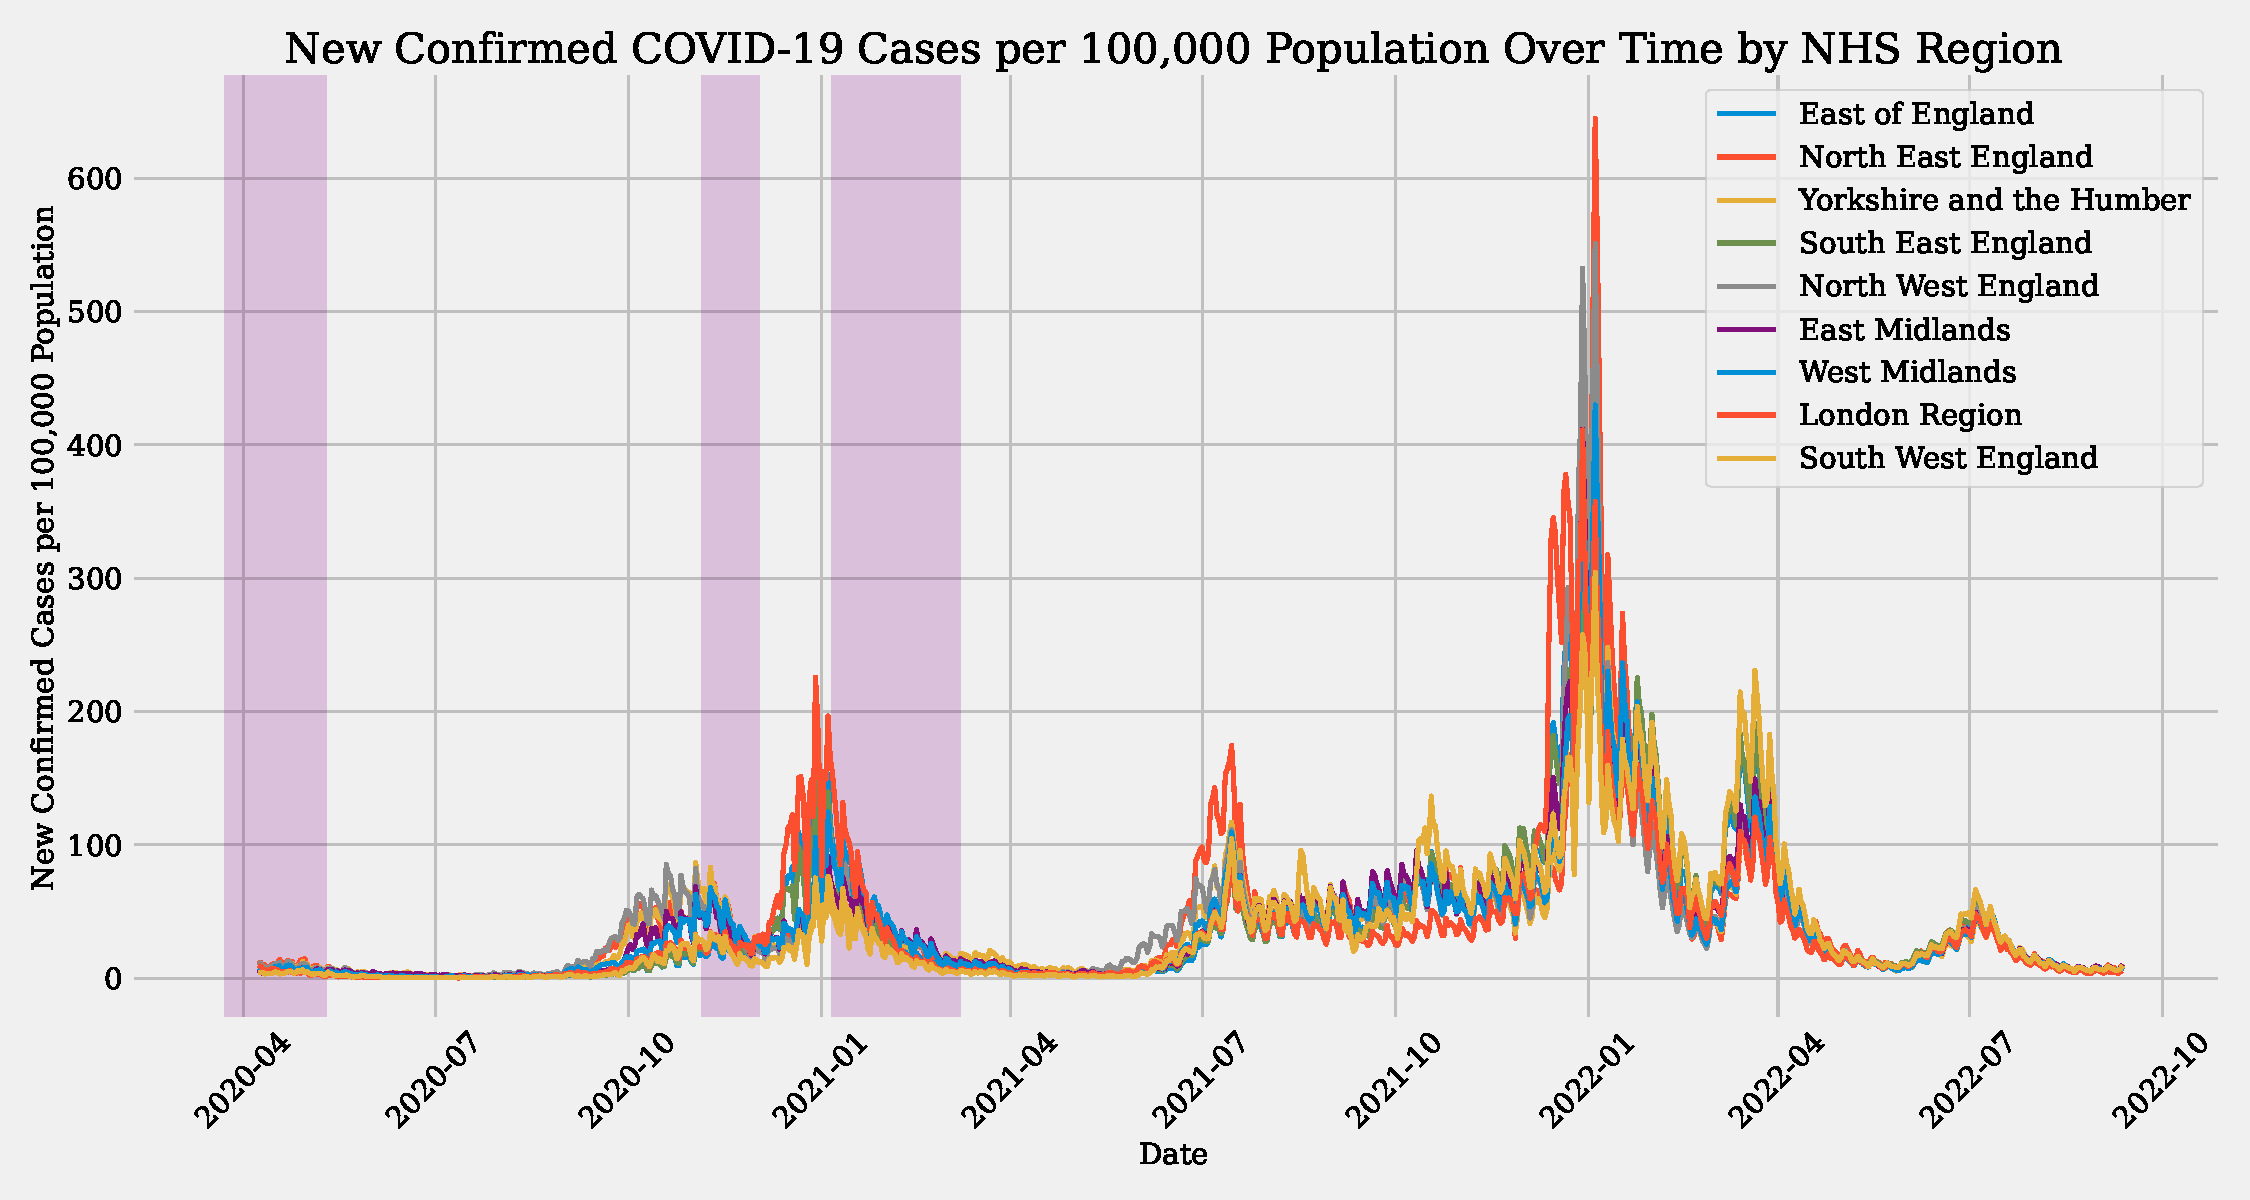
\includegraphics[width=0.9\textwidth]{"images/new_confirmed_per_100k.pdf"}
    \caption{new confirmed COVID-19 cases per 100k people overtime by NHS regions.}
    \label{fig:new_confirmed_per_100k}
\end{figure}
\section{Research Question}

Given the complexity of the COVID-19 pandemic and its diverse impacts in different geographical regions, this study seeks to address a fundamental question:

\begin{itemize}
    \item How can data-driven methods, specifically physics-informed neural networks (PINN) and its variant, be effectively utilised to understand and model the dynamic behaviour of COVID-19 across all NHS regions in the United Kingdom?
\end{itemize}

\section{Contributions}

This research contributes significantly to the field of epidemiological modelling and public health policy in the context of the COVID-19 pandemic, with the following key advances:

\begin{enumerate}
    \item The development of a sophisticated modelling framework that makes use of physics-informed neural networks (PINN) and its variants to capture the COVID-19 dynamics uniquely in each NHS region. This approach allows for the accommodation of region-specific data, including infection rates, recovery rates, and intervention effects, providing a tailored understanding of the pandemic's behaviour in diverse settings.

    \item  A novel methodological advancement to address the challenges posed by reporting delays and data anomalies common in epidemiological data. By integrating these factors into the model, this research improves the precision and reliability of COVID-19 forecasts, offering more precise guidance for public health decision making.

    \item Through the application of PINN and UDE, this study provides critical insight into the effectiveness of various public health interventions in the NHS regions. By simulating different scenarios, the research identifies optimal strategies to mitigate the spread of COVID-19, contributing valuable knowledge to the planning and implementation of health measures.
\end{enumerate}

 Using these computational methods, this research offers significant information on the COVID-19 pandemic, helping to formulate targeted and effective public health responses.


\section{Methodology}
This section describes the methodology used in this study. Two methods were implemented to show how deep learning can be used in conjunction with an epidemiological model to understand the dynamics of the disease in various regions. The methods were trained using two different programming languages and libraries. The first was the PINNs was trained using pytorch while the UDE was trained in julia programming language.

\subsection{mathematical modelling of infectious disease}
In the context of the COVID-19 pandemic, accurate epidemiological modelling and resource demand forecasting play a crucial role in informing healthcare professionals and governments on how to effectively manage overburdened healthcare systems. The use of predictive models has been crucial in the context of the COVID-19 pandemic, helping healthcare professionals and governments effectively manage overburdened healthcare systems. The most common model is the Susceptible-Infectious-Removed (SIR) epidemic model. It was proposed by Kermack-Mckendrick in 1927 \cite{kermack1927contribution}. 

\subsection{SIR and SEIRD epidemiological dynamic models}
The SIR models are pivotal in understanding the dynamics of infectious diseases, such as COVID-19, providing insight into how diseases spread and recede within populations. These models help predict the number of individuals affected by a disease over time and are crucial for public health planning and intervention strategies. There are other variants of the model designed for various assumptions and for solving different problems. SEIR, SIS    

The SIR model compartmentalises the population into three categories: Susceptible (S), Infectious (I), and Recovered (R) individuals. The transitions between these categories are governed by a set of ordinary differential equations (ODEs) as follows:

\begin{equation}
    \begin{align}
        \frac{dS}{dt} &= -\beta \frac{SI}{N} \\
        \frac{dI}{dt} &= \beta \frac{SI}{N} - \gamma I \\
        \frac{dR}{dt} &= \gamma I
    \end{align}
\end{equation}

where $S$ represents the number of susceptible individuals who are not yet infected but can be, $I$ denotes the number of infectious individuals who can transmit the disease to susceptible individuals and recover, and $R$ represents the number of recovered individuals who are immune to the disease. Parameters $\beta$ and $\gamma$ represent the transmission rate and recovery rate, respectively. The SIR model is a simple and effective tool for understanding the dynamics of infectious diseases and has been widely used to model the spread of various diseases, including COVID-19.

Equation (1) is governed by the following initial conditions: $S(t_0) > 0$, $I(t_0) \geq 0$, and $R(t_0) \geq 0$, where $t_0$ represents the initial point in time. These conditions ensure that the population starts with a positive number of susceptible individuals and non-negative numbers of infectious and recovered individuals. 

\begin{figure}[h!]
    \centering
    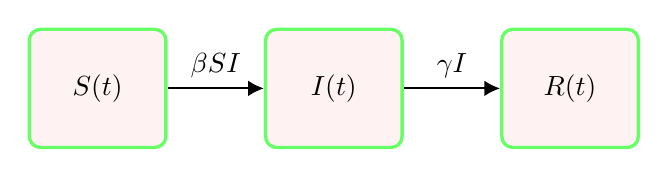
\begin{tikzpicture}[node distance=3cm, auto, thick]
        % Define block styles
        \tikzstyle{roundnode} = [circle, draw=green!60, fill=green!5, very thick, minimum size=1cm, text centered]
        \tikzstyle{squarednode} = [rectangle, draw=green!60, fill=red!5, very thick, text width=1.5cm, text centered, rounded corners, minimum height=1.5cm]
        \tikzstyle{line} = [draw, -{Latex[length=2mm, width=2mm]}]

        % Define nodes
        \node [squarednode] (S) {\( S(t) \)};
        \node [squarednode, right of=S] (I) {\( I(t) \)};
        \node [squarednode, right of=I] (R) { \( R(t) \)};

        % Connect nodes with paths
        \path [line] (S) -- node { \( \beta S I \) } (I);
        \path [line] (I) -- node { \( \gamma I \) } (R);

    \end{tikzpicture}
    \caption{Compartmental flow of the SIR model for infection transmission dynamics.}
\end{figure}

The model operates under the assumption of population conservation, formulated as:
\begin{equation}
    S(t) + I(t) + R(t) = N, \quad \forall t \geq t_0,
\end{equation}
where $N$ denotes the total constant population size. This equation implies that the total number of individuals in the model remains constant over time, encapsulating the assumption that the timescale of the epidemic's evolution is significantly shorter than the average lifespan of individuals in the population. Consequently, demographic processes such as births and natural deaths are not considered under the premise that their impact on the total population size is negligible within the timeframe of the epidemic's spread.

% \begin{table}[h!]
%     \centering
%     \begin{tabular}{ll}
%     \toprule
%     \textbf{Parameter} & \textbf{Definition} \
%     \midrule
%     $\beta$ & Transmission rate \
%     $\gamma$ & Recovery rate \
%     \bottomrule
%     \end{tabular}
%     \caption{Parameters of the SIR Model}
% \end{table}
    
The SIR model is fundamental in epidemiology for its simplicity and effectiveness in capturing the basic dynamics of disease spread. However, it assumes lifelong immunity post-recovery, which may not apply to all diseases, including COVID-19.

To account for the characteristics of COVID-19, including the existence of a latent period and the possibility of death, the SEIRD model extends the SIR framework by including two additional compartments: Exposed (E) and Dead (D) individuals. The SEIRD model is described by the following differential equations:

\begin{equation}
    \begin{align}
        \frac{dS}{dt} &= -\beta \frac{SI}{N} \\
        \frac{dE}{dt} &= \beta \frac{SI}{N} - \sigma E \\
        \frac{dI}{dt} &= \sigma E - \rho I - \alpha I \\
        \frac{dR}{dt} &= \rho I, \\
        \frac{dD}{dt} &= \alpha I,
    \end{align}
\end{equation}

where $E$ represents the number of exposed individuals who are infected but not yet infectious, and $D$ represents the number of deceased individuals. The parameters $\sigma$, $\rho$, and $\alpha$ represent the rate of exposed individuals becoming infectious, the recovery rate, and the mortality rate, respectively. The total population size is denoted by $N = S + E + I + R + D$. The SEIRD model provides a more comprehensive representation of disease dynamics and is particularly useful to capture the spread of COVID-19, which exhibits a latent period and the possibility of death. This model more accurately reflects the disease dynamics of COVID-19 by considering the exposed phase, during which individuals are infected but not yet infectious, and the mortality due to the disease. The addition of these compartments allows for a more nuanced understanding of the pandemic progression and the impact of interventions such as social distancing, vaccination, and treatment strategies.


\begin{figure}[h!]
    \centering
    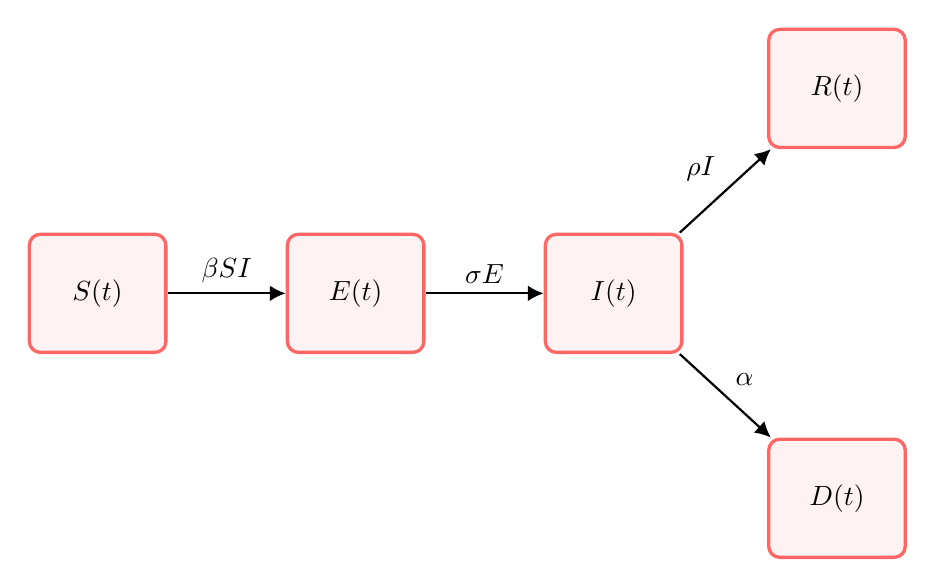
\begin{tikzpicture}[node distance=1.5cm, auto, thick]
        % Define block styles
        \tikzstyle{roundnode} = [circle, draw=green!60, fill=green!5, very thick, minimum size=1cm, text centered]
        \tikzstyle{squarednode} = [rectangle, draw=red!60, fill=red!5, very thick, text width=1.5cm, text centered, rounded corners, minimum height=1.5cm]
        \tikzstyle{line} = [draw, -{Latex[length=2mm, width=2mm]}]
    
        % Define nodes
        \node [squarednode] (S) {\( S(t) \)};
        \node [squarednode, right=of S] (E) {\( E(t) \)};
        \node [squarednode, right=of E] (I) {\( I(t) \)};
        \node [squarednode, above right=of I] (R) { \( R(t) \)};
        \node [squarednode, below right=of I] (D) { \( D(t) \)};
        
        % Connect nodes with paths
        \path [line] (S) -- node { \( \beta S I \) } (E);
        \path [line] (E) -- node { \(  \sigma E \) } (I);
        \path [line] (I) -- node { \( \rho I\) } (R);
        \path [line] (I) -- node { \( \alpha \) } (D);

    \end{tikzpicture}
    \caption{Compartmental flow of the SEIRD model for COVID-19 transmission dynamics.}
\end{figure}

\subsection{Physics-Informed Neural Networks}

Physics-Informed Neural Networks (PINNs) embody a novel approach to embedding a priori system knowledge, such as fundamental physical principles or domain expertise, directly into the learning mechanism of deep neural networks. This incorporation is typically achieved through the utilisation of ordinary or partial differential equations (ODEs/PDEs) within the loss function formulation. During training, PINNs aim not only to adjust network weights and biases but also to refine parameters within the encapsulated physical laws. The composite loss function encompasses two primary components: the loss of fidelity to the data ($L_{\text{data}}$) and the residual loss based on physics ($L_{\text{residual}}$), the latter serving as a regularisation mechanism that enforces adherence to established differential equations.

Consider a system governed by a set of first-order ODEs expressed as:
\begin{equation}
\frac{\partial U}{\partial t}(t) + F(U(t); \lambda) = 0, \quad t \in [t_0, T],
\end{equation}
where $U(t) = [u_1(t), \ldots, u_n(t)]^T$ and $F(U) = [f_1(U), \ldots, f_n(U)]^T$ with $u_i \in \mathbb{R}$ and $f_i: \mathbb{R}^n \rightarrow \mathbb{R}$ for $i = 1, \ldots, n$. The interval $[t_0, T]$ denotes the time domain from initial to final time, with $\lambda \in \mathbb{R}^k$ representing unknown parameters of the system. The observed data $U_s$ at times $t_1, \ldots, t_m$ are used to determine $\lambda$, leading to the data loss:
\begin{equation}
L_{\text{data}} = \sum_{s=1}^{m} \|U(t_s) - U_s\|^2.
\end{equation}

Traditionally, the optimal parameter vector $\lambda$ is identified by minimising $L_{\text{data}}$, thus obtaining a solution $U(t)$ that closely aligns with the observed data in terms of least squares deviations. PINNs uses a general neural network framework, denoted as $NN_{\omega,b}(t): \mathbb{R} \rightarrow \mathbb{R}^n$, which approximates the solution $U(t): \mathbb{R} \rightarrow \mathbb{R}^n$ of the ODE system. The network's weights $\omega$ and biases $b$ are optimized to minimize the mean squared error (MSE) between the network's predictions and the observed data:

\begin{equation}[h]
    MSE_{\omega,b}^U = \frac{1}{m} \sum_{s=1}^{m} \|NN_{\omega,b}(t_s) - U_s\|^2.
\end{equation}

The residual loss, derived from the ODE system, is formulated as follows:
\begin{equation}
F(NN_{\omega,b}, t; \lambda) = \frac{\partial NN_{\omega,b}}{\partial t}(t) + F(NN_{\omega,b}(t); \lambda),
\end{equation}
enabling the extension of $NN_{\omega,b}$ into a PINN by incorporating the residual term into the loss function. Through automatic differentiation, the neural network computes derivatives of its output with respect to its input, thus ensuring compliance with the ODE dynamics by enforcing $F(NN_{\omega,b}, t; \lambda) = 0$ for all $t \in [t_0, T]$. Consequently, PINNs facilitate the simultaneous identification of optimal neural network parameters ($\omega$ and $b$) and ODE parameters ($\lambda$), by minimising the combined loss:
\begin{equation}
\text{arg min}_{\omega, b, \lambda} \left( MSE_{\omega,b}^U + MSE_{\omega,b,\lambda}^F \right),
\end{equation}
where $MSE_{\omega,b,\lambda}^F$ represents the mean squared residual error, integrating the system's dynamics into the optimization process.

\begin{figure}
    \centering
    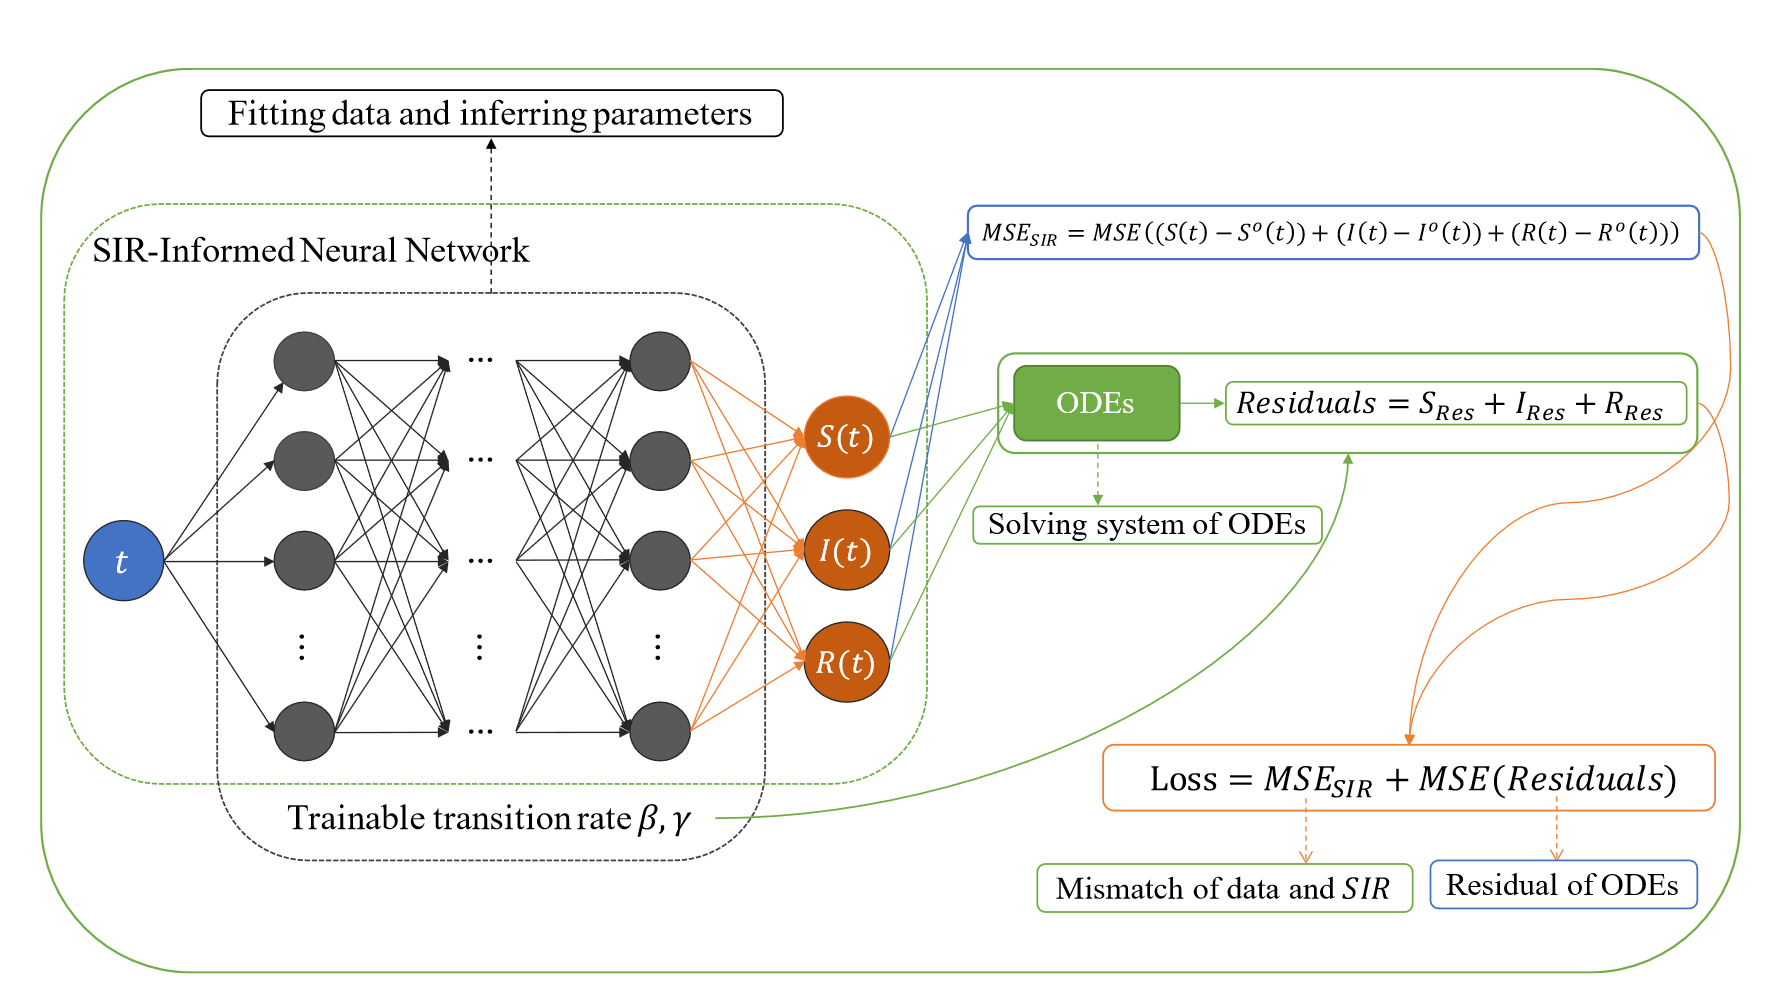
\includegraphics[width=0.8\textwidth]{images/image.png}
    \caption{Caption}
    \label{fig:enter-label}
\end{figure}

\subsection{Integration of the SIR Model into Physics-Informed Neural Networks}
This subsection elucidates the methodology for embedding the SIR (Susceptible, Infected, Recovered) model within the framework of Physics-Informed Neural Networks (PINNs), leveraging it as foundational knowledge. It involves the estimation of dynamic parameters characteristic of the SIR model, encompassing the formulation and computation of both the data loss function and the physical residual terms.

\subsection{Neural Network Architecture for the SIR Model}
As illustrated in Figure 4, the architecture employs a densely connected neural network, highlighted by a black dashed border, for approximating the state variables \(S(t)\), \(I(t)\), and \(R(t)\) at any given time \(t\), in accordance with the governing equations of the SIR model. The objective is to minimise the residual of the ordinary differential equations (ODEs) specific to the SIR model, facilitating adherence to the predefined dynamics.

The functional representation within the network, aiming to minimize the residuals, is given by:
\begin{equation}
    F(NN_{\omega,b}, t; \beta, \gamma) = \left[ \begin{array}{c}
        \frac{dS(t)}{dt} + \frac{\beta S(t)I(t)}{N} \\
        \frac{dI(t)}{dt} - \frac{\beta S(t)I(t)}{N} + \gamma I(t) \\
        \frac{dR(t)}{dt} - \gamma I(t)
    \end{array} \right].
\end{equation}

The mean squared error for the residuals in this study is computed as:
\begin{equation}
    MSE_{SIR} = MSE_{S,residual} + MSE_{I,residual} + MSE_{R,residual},
\end{equation}
where
\begin{align}
    MSE_{S,residual} &= \frac{1}{q} \sum_{i=1}^{q} \left| \frac{dS(t_i)}{dt_i} + \frac{\beta S(t_i)I(t_i)}{N} \right|^2, \\
    MSE_{I,residual} &= \frac{1}{q} \sum_{i=1}^{q} \left| \frac{dI(t_i)}{dt_i} - \frac{\beta S(t_i)I(t_i)}{N} + \gamma I(t_i) \right|^2, \\
    MSE_{R,residual} &= \frac{1}{q} \sum_{i=1}^{q} \left| \frac{dR(t_i)}{dt_i} - \gamma I(t_i) \right|^2.
\end{align}

In this model, \(q\) represents the total number of discrete time intervals, with each interval chosen to align with the natural day units, thus setting \(\Delta t = 1\). This temporal discretization aligns with the observed data frequency, ensuring that the time steps between observations are consistent. The mean squared error (MSE) for the data within the SIR model framework is defined as:
\begin{equation}
    MSE_{data} = MSE_{S,data} + MSE_{I,data} + MSE_{R,data},
\end{equation}
where:
\begin{align}
    MSE_{S,data} &= \frac{1}{s} \sum_{i=1}^{s} \left|S(t_i) - S_{o,i}\right|^2, \\
    MSE_{I,data} &= \frac{1}{s} \sum_{i=1}^{s} \left|I(t_i) - I_{o,i}\right|^2, \\
    MSE_{R,data} &= \frac{1}{s} \sum_{i=1}^{s} \left|R(t_i) - R_{o,i}\right|^2.
\end{align}
Here, \(S_{o,i}\), \(I_{o,i}\), and \(R_{o,i}\) represent the observed data points for susceptible, infected, and recovered individuals at time \(t_i\), respectively, with \(s\) denoting the total number of observed data points. The overall loss function combines data and residual errors, guiding the optimisation of network weights, biases, and dynamic model parameters.

The optimization problem is formulated as:
\begin{equation}
    \text{minimize}_{\omega, b, \beta, \gamma} \; (MSE_{data} + MSE_{SIR}),
\end{equation}

The algorithm below details the process for determining trainable parameters, including both NN) weights and biases and SIR model parameters, using PINNs. The algorithm inputs a time point \(t\) and outputs the compartmental values of the SIR model at \(t\). Initial values for weights \(\omega\) and biases \(b\) are set using the Xavier initialisation \cite{kumar2017weight}, while \(\beta\) and \(\gamma\) were selected to be 0.25 and 0.15 respectively ensuring reproducibility by fixing these values throughout the experiments.

\begin{algorithm}
    \label{algo:1}
    \caption{PINN Training for Epidemic Modelling}
    \begin{algorithmic}
        \Require Training data tensors $\mathbf{S}_{data}$, $\mathbf{I}_{data}$, $\mathbf{R}_{data}$, time tensor $\mathbf{t}_{data}$, population size $N$.
        \State Initialise PINN model parameters with Xavier initialisation.
        \State Set up Adam optimiser with defined learning rate and weight decay parameters.
        \For{$epoch = 1$ to $num\_epochs$}
            \State Perform forward propagation to predict $\mathbf{S}_{pred}$, $\mathbf{I}_{pred}$, $\mathbf{R}_{pred}$ using current model state.
            \State Utilise automatic differentiation to calculate gradients.
            \State Compute $MSE_{SIR}$ between the predictions of the model and the actual data.
            \State Calculate mean squared error for the residuals, $MSE_{residuals}$.
            \State Aggregate loss as $Loss = MSE_{SIR} + MSE_{residuals}$.
            \State Update model parameters using the backpropagation and optimisation step.
        \EndFor
    \end{algorithmic}
\end{algorithm}

\subsection{Universal Differential Equations}
The Universal Differential Equation (UDE) \cite{rackauckas2020universal} framework introduces a novel integration of universal approximators within the structure of forced stochastic delay Partial Differential Equations (PDEs). This innovative approach allows the modelling of complex dynamical systems by leveraging the power of universal approximators to encapsulate a wide range of functional behaviours within specified parametric limits. Specifically, the UDE formulation is mathematically expressed as follows:
\begin{equation}
N[u(t), u(\alpha(t)), W(t), U_{\theta}(u, \beta(t))] = 0,
\end{equation}
where \(u(t)\) denotes the state of the system at time \(t\), \(\alpha(t)\) represents a delay function introducing temporal dependencies, and \(W(t)\) signifies the Wiener process, incorporating stochastic elements into the system dynamics. Here, \(N[\cdot]\) is a nonlinear operator, and \(U_{\theta}(\cdot)\) denotes a universal approximator, parameterized by \(\theta\), capable of emulating an extensive array of functional forms. This framework effectively bridges the gap between deep learning models and physics-based knowledge, offering a versatile platform for the exploration and integration of empirical data and theoretical principles.


In the context of employing UDEs for modelling epidemic dynamics, specifically using the SEIRD model, training involves minimisation of a cost function \(C(\theta)\) relative to the solution \(u_{\theta}(t)\) of the differential equation and the parameter set \(\theta\). The cost function, often chosen to be the Euclidean distance between the model's predictions and observed data at discrete time points, is defined as

\begin{equation}
    C(\theta) = \sum_{i} \lVert u_{\theta}(t_i) - d_i \rVert,
\end{equation}

where \((t_i, d_i)\) denotes the observed data points.

Optimisation techniques such as stochastic gradient descent, ADAM and LBFGS are utilised for model training, necessitating efficient gradient calculation of \(u_{\theta}(t)\) with respect to \(\theta\). Adjoint methods, recognised for their computational efficiency, especially in models with a large number of parameters and state variables, become instrumental. Unlike traditional numerical or forward-sensitivity approaches, the computational burden of adjoint methods does not increase multiplicatively with the increase in parameters or state variables, rendering them empirically more efficient for complex and high-dimensional models.

\subsubsection{Neural Network Architecture for UDE-based SEIRD Model}

The UDE approach for the SEIRD epidemic model leverages a distinct neural network architecture for each of the model's parameters: \(\beta\) (transmission rate), \(\gamma\) (recovery rate), \(\delta\) (mortality rate), and \(\alpha\) (exposure rate). These neural networks are designed to capture the temporal dynamics of the epidemic's parameters, allowing for a flexible adaptation to observed data. The neural network for each parameter is constructed using a series of densely connected layers with the following specifications.

\begin{itemize}
    \item \textbf{Input Layer:} A single input neuron to accept time \(t\) as the input, reflecting the time-dependent nature of the parameter being modelled.
    \item \textbf{Hidden Layers:} Three hidden layers, each comprising 50 neurons. These layers employ the \texttt{tanh\_fast} activation function, provided by the Lux library, to introduce nonlinearity into the learning process.
    \item \textbf{Output Layer:} A single output neuron to predict the parameter value at time \(t\).
\end{itemize}
The \texttt{tanh\_fast} activation function employed within the neural network layers is a variant of the traditional hyperbolic tangent function. Mathematically, the standard \(\tanh\) function is defined as:

\begin{equation}
    \tanh(x) = \frac{e^{x} - e^{-x}}{e^{x} + e^{-x}},
\end{equation}

which smoothly maps input values to the \((-1, 1)\) range, introducing non-linearity into the neural network. The \texttt{tanh\_fast} version is designed to approximate this behaviour with a computationally efficient implementation, crucial to reducing training time without significantly sacrificing the accuracy of the model or the smooth gradient properties of the function.

The architecture for each parameter (\(\beta\), \(\gamma\), \(\delta\), \(\alpha\)) is instantiated through the function (\(NN\)), which encapsulates the design of the network in a cohesive and reusable structure. This function returns the initialised neural network alongside its parameters and state, ready for integration into the SEIRD model.

Within the SEIRD model, the neural networks for \(\beta\), \(\gamma\), \(\delta\), and \(\alpha\) dynamically predict the rates based on the current simulation time \(t\), which are then used to compute the transitions between compartments (susceptible, exposed, exposed, recovered, deceased) according to the dynamics of the model. The training process involves adjusting the neural networks' parameters to minimise a loss function that captures the discrepancy between the model's predictions and the observed data on infected and deceased populations. This optimisation is performed using gradient-based methods, with gradients efficiently computed via adjoint methods to account for the full trajectory of the model's predictions.

The loss function is composed of the following elements: 1. The mean squared error (MSE) between the logarithm of the observed data (infected and deceased) and the model predictions. This component aims to minimize the relative error, taking into consideration the magnitude of the data. 2. The MSE between the predicted reproduction number \(R_t\) and the desired value (ideally 1.0). This component encourages the model to be consistent with epidemiological principles.

The neural network architecture delineated above underpins the UDE approach to modelling the dynamics of the, embodying a sophisticated method for capturing temporal variations in critical epidemiological parameters. Through this architecture, the model adapts to changing conditions, offering insight into the progression and potential control measures for the epidemic.

The optimisation process for the UDE-based SEIRD model involves a multistage strategy to refine the parameters of the neural networks that dynamically estimate the epidemic parameters (\(\beta\), \(\gamma\), \(\delta\), and \(\alpha\)). This process is critical to ensuring that the model accurately reflects the observed data and adheres to the underlying epidemiological dynamics.

The optimisation process consists of two main stages, where different optimization algorithms are used to balance the exploration and exploitation of the parameter space. In the first stage, the ADAM optimiser is used with a learning rate of \(0.0001\). This optimiser is known for its efficiency in navigating large parameter spaces. The primary goal of this stage is to quickly converge towards a viable parameter region. The ADAM optimiser's adaptive learning rate mechanism is employed to mitigate the risk of premature convergence. In the second stage, after the initial optimisation with ADAM, the BFGS algorithm is employed to further refine the parameter estimates. BFGS is a quasi-Newton method that is chosen for its precision in fine-tuning, particularly in the vicinity of the optimum. This is achieved through its line-search mechanism and efficient utilisation of gradient information.

The optimisation process is facilitated by the \texttt{OptimizationFunction} and \texttt{OptimizationProblem} constructs, which encapsulate the loss function and the parameter space of the model, respectively. A custom callback function monitors the optimisation progress, logging the loss at each iteration and enabling early termination if desired. The optimisation commences with the ADAM algorithm for a maximum of 1000 iterations, followed by a transition to the BFGS algorithm for up to 100 iterations. This staged approach allows for a comprehensive exploration and exploitation of the parameter space, ensuring a robust fit to the observed epidemic data.

This comprehensive approach to model training not only ensures an accurate fit to the data but also maintains the epidemiological relevance of the parameter estimates, facilitating a robust analysis of the epidemic's dynamics.

\begin{algorithm}[h]
    \label{algo:2}
    \caption{UDE Training for Epidemic Modeling}
    \begin{algorithmic}

        \Require data for $\mathbf{I}_{data}$, $\mathbf{R}_{data}$, population size $N$,\\
        initial conditions $u(t_0) = [S_0, E_0, I_0, R_0, D_0]$ for SEIRD compartments.
        
        \State Normalize and partition the data for input into the UDE model for $t_1, t_2, \ldots, t_n$.
        
        \State Construct Universal Approximators (UAs) $UA_{\beta}(t;\theta_{\beta})$, $UA_{\gamma}(t;\theta_{\gamma})$, $UA_{\delta}(t;\theta_{\delta})$, $UA_{\alpha}(t;\theta_{\alpha})$ for the dynamic parameters of the model.

        \For{$epoch = 1$ to $num\_epochs$}

            \State Integrate UAs into SEIRD equations to define the dynamics of the system for the current epoch.

            \State Solve the SEIRD model based on UDE to predict $\mathbf{S}_{pred}$, $\mathbf{I}_{pred}$, $\mathbf{R}_{pred}$, $\mathbf{E}_{pred}$, $\mathbf{D}_{pred}$.

            \State compute gradients $\frac{d\mathcal{L}}{d\theta}$ of the loss function $\mathcal{L}(\theta)$ with respect to $\theta$ with adjoint methods.

            \State Compute loss $\mathcal{L}(\theta)$ combining prediction errors and regularizations of the parameter trajectory.

            \State Update parameters $\theta$ using gradient-based optimisation (e.g. ADAM, LBFGS) or both
        \EndFor
    \end{algorithmic}
\end{algorithm}




\section{Results and Discussion}

\subsection{Data preprocessing}
The utilized data consisted of the daily records of infections, deaths, cumulative infections, and cumulative deaths for all available regions. The training set for the SIR model was selected from May 1, 2020, to December 1, 2021. The data is readly available online on the COVID-19 NHS repository. various preprocessing steps was employed to carefully curate the data based on each region and analysis was done on the data.

Specifically, the dataset for all the regions encapsulates the cumulative counts of infectious cases (\(I_c\)), recovered individuals (\(R_c\)), and deceased cases (\(D_c\)). In accordance with the compartmental definitions within the SIR model, the recovered compartment (\(R\)) combines both the number of individuals who have recovered and the number of fatalities caused by the virus, expressed as \(R = R_{\text{recovered}} + D_{\text{death}}\). Given that the \(R\) compartment does not experience any flows, it is equivalent to the cumulative removed population, \(R = R_{\text{ec}}\).

Using the data, the values for the removed (\(R\)), infectious (\(I\)), and susceptible (\(S\)) compartments are derived as follows: \(R = R_{\text{recovered}} + D_{\text{death}}\), \(I = I_c - R\), and \(S = N - I - R\), where \(N\) represents the total population. This procedure was adopted from  \cite{amaral2021towards}, where \(C\) symbolizes the total confirmed cases and \(T = 21\) days is assumed to be the approximate recovery period for the infection. Consequently, the population removed at any given time \(t\) is calculated as \(R(t) = C(t - T) - D(t - T)\), and the infectious population is obtained by \(I(t) = C(t) - D(t) - R(t)\). 

The 7-day moving average was applied to the data to remove the noise available in the data. Data were also used for the experiment that involves the UDE, where a 40-day training period was used. The time period of the model was different and this discrepancy was detected in the results.

\begin{figure*}[ht]
    \centering
    \begin{subfigure}[t]{0.45\textwidth}
        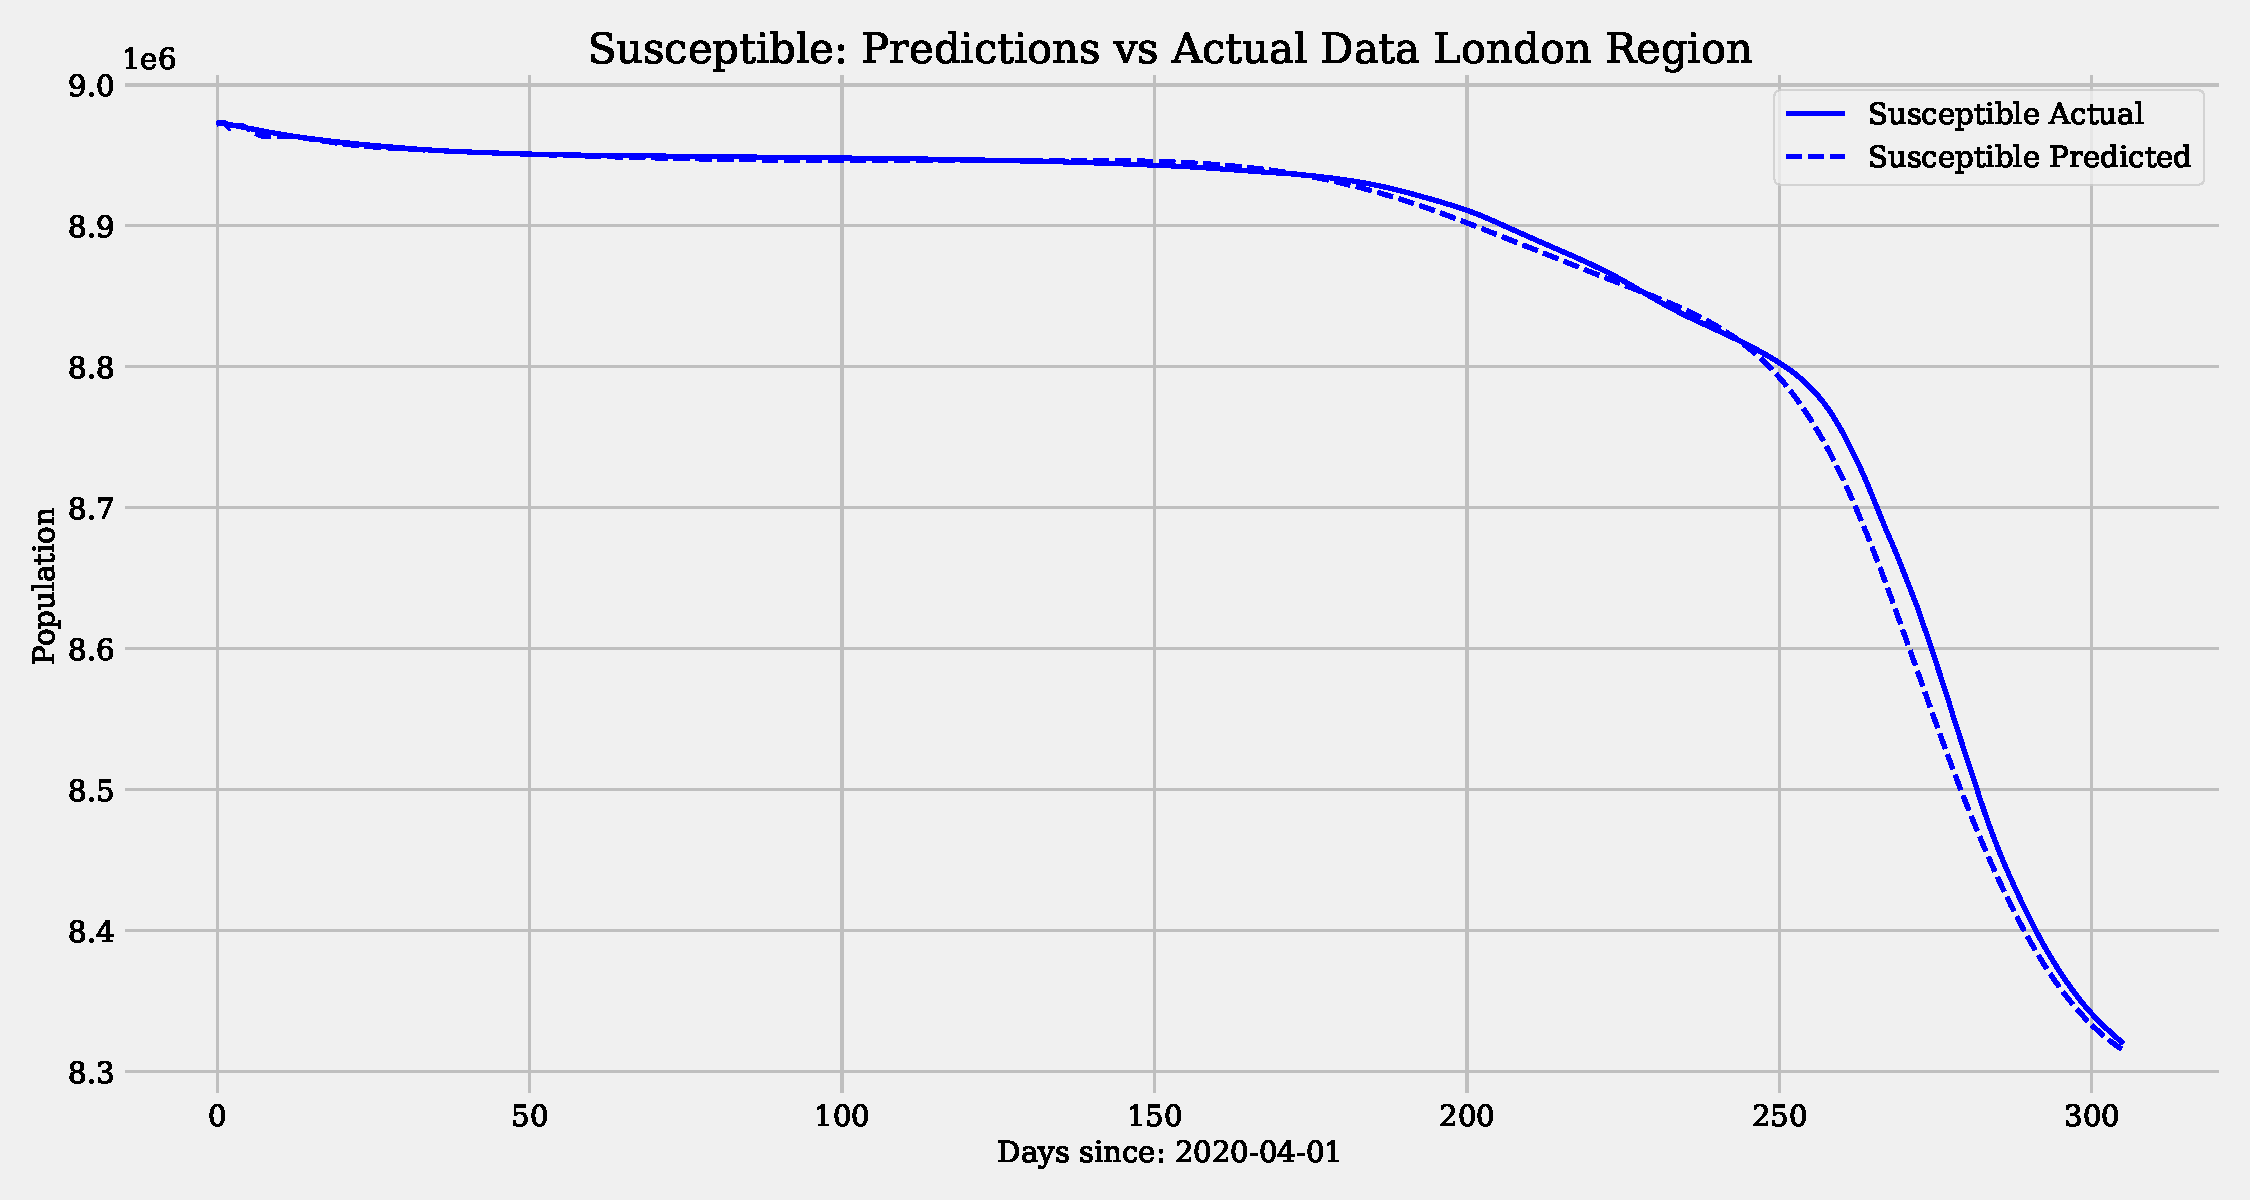
\includegraphics[width=\textwidth]{images/pinn/S_predictions_London Region.pdf}
        \caption{Predicted number of susceptible individuals}
        \label{fig:S_predictions_London}
    \end{subfigure}
    \hfill % Ensures that the figures are spaced out evenly
    \begin{subfigure}[t]{0.45\textwidth}
        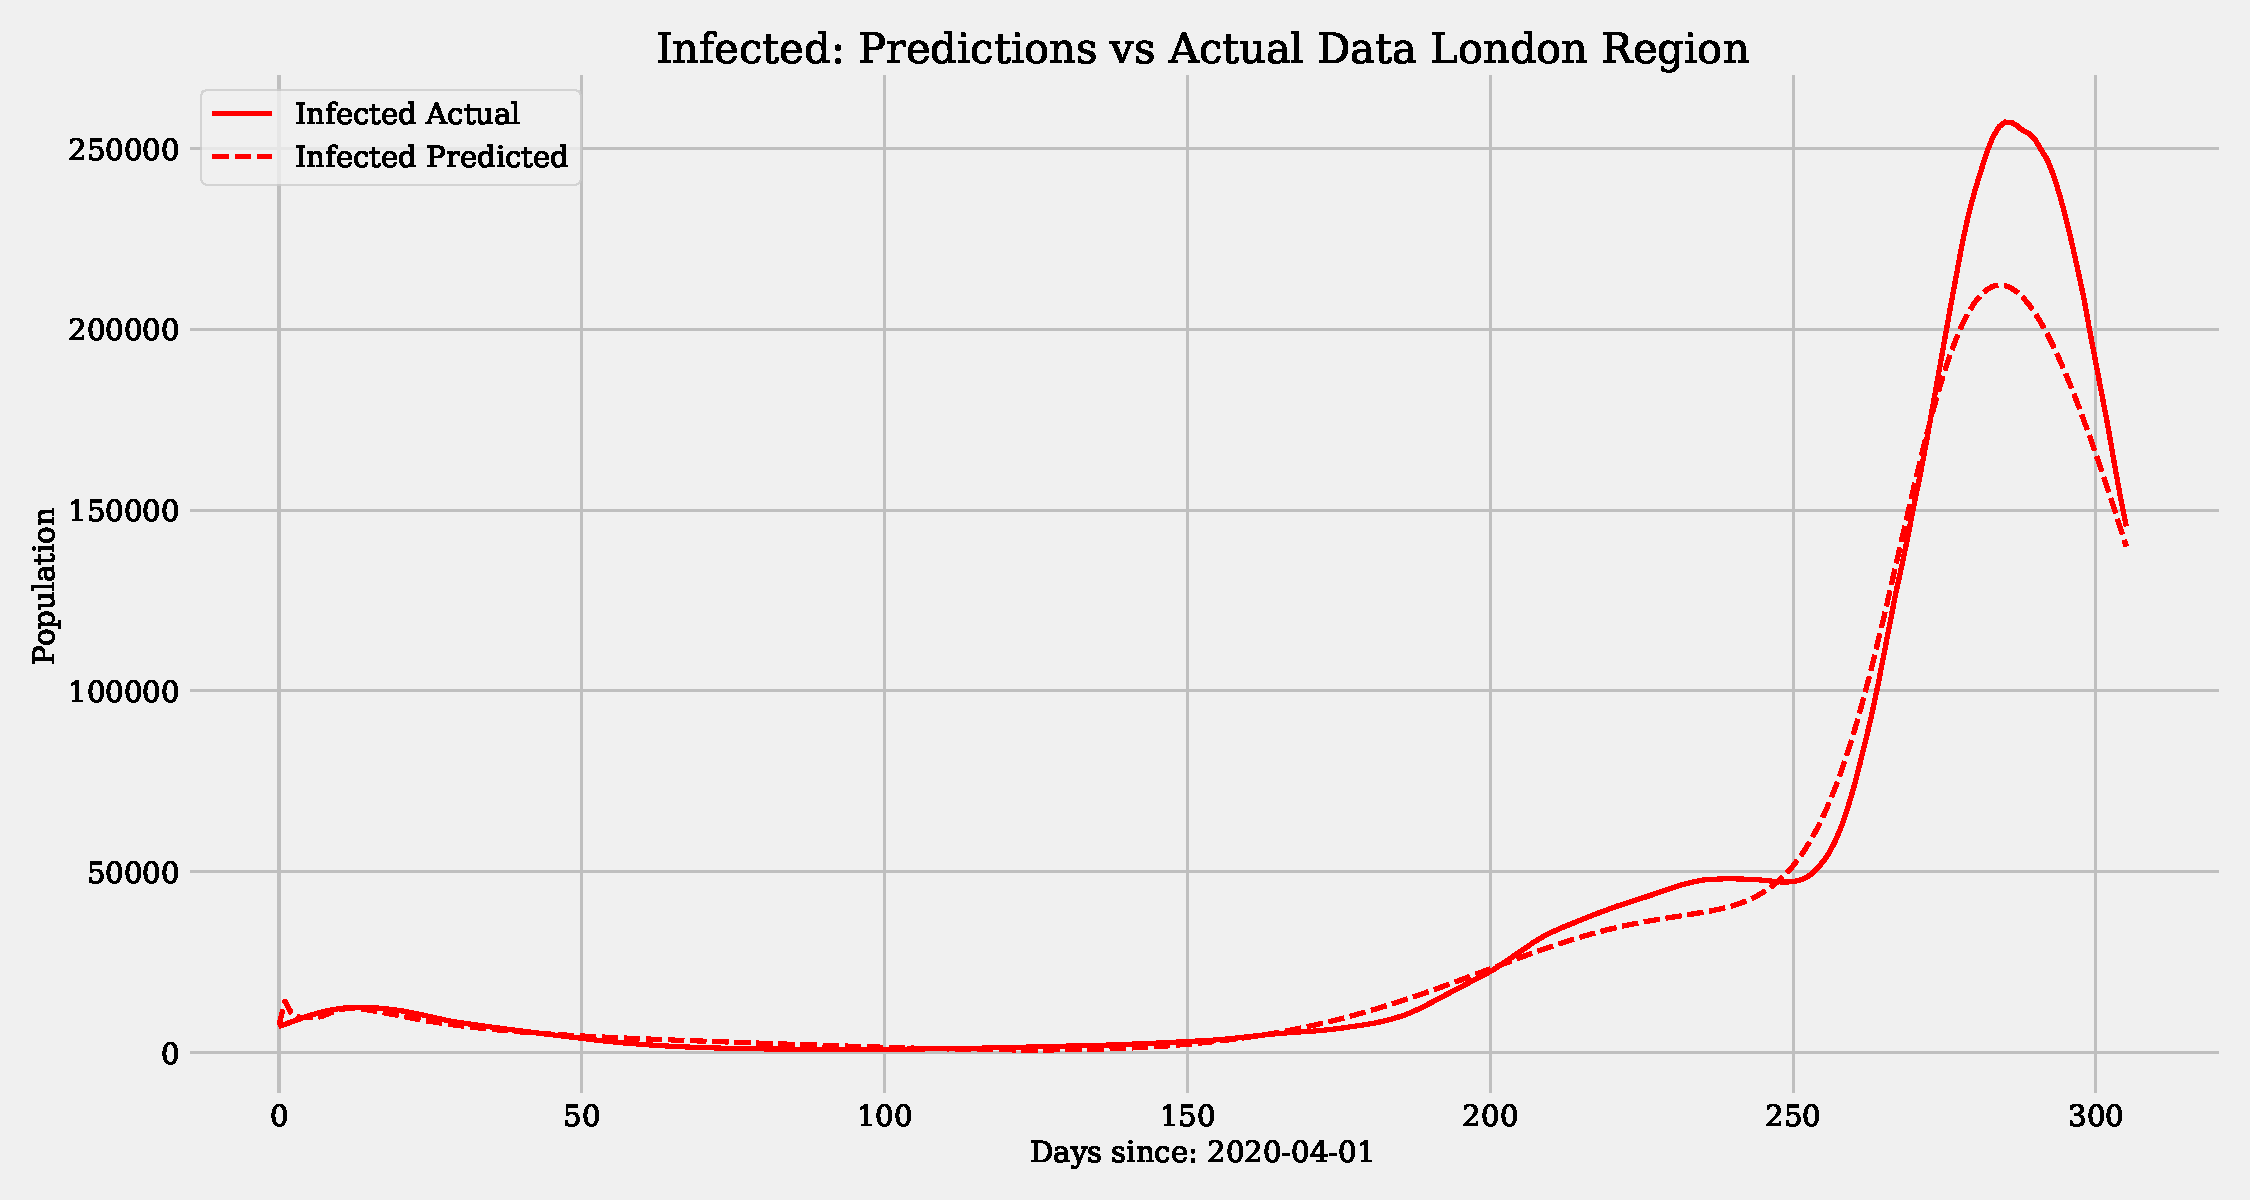
\includegraphics[width=\textwidth]{images/pinn/I_predictions_London Region.pdf}
        \caption{Predicted number of infectious individuals}
        \label{fig:I_predictions_London}
    \end{subfigure}
    
    % Adds a bit of vertical space between the rows of figures
    \vspace{0.5cm}
    
    \begin{subfigure}[t]{0.45\textwidth}
        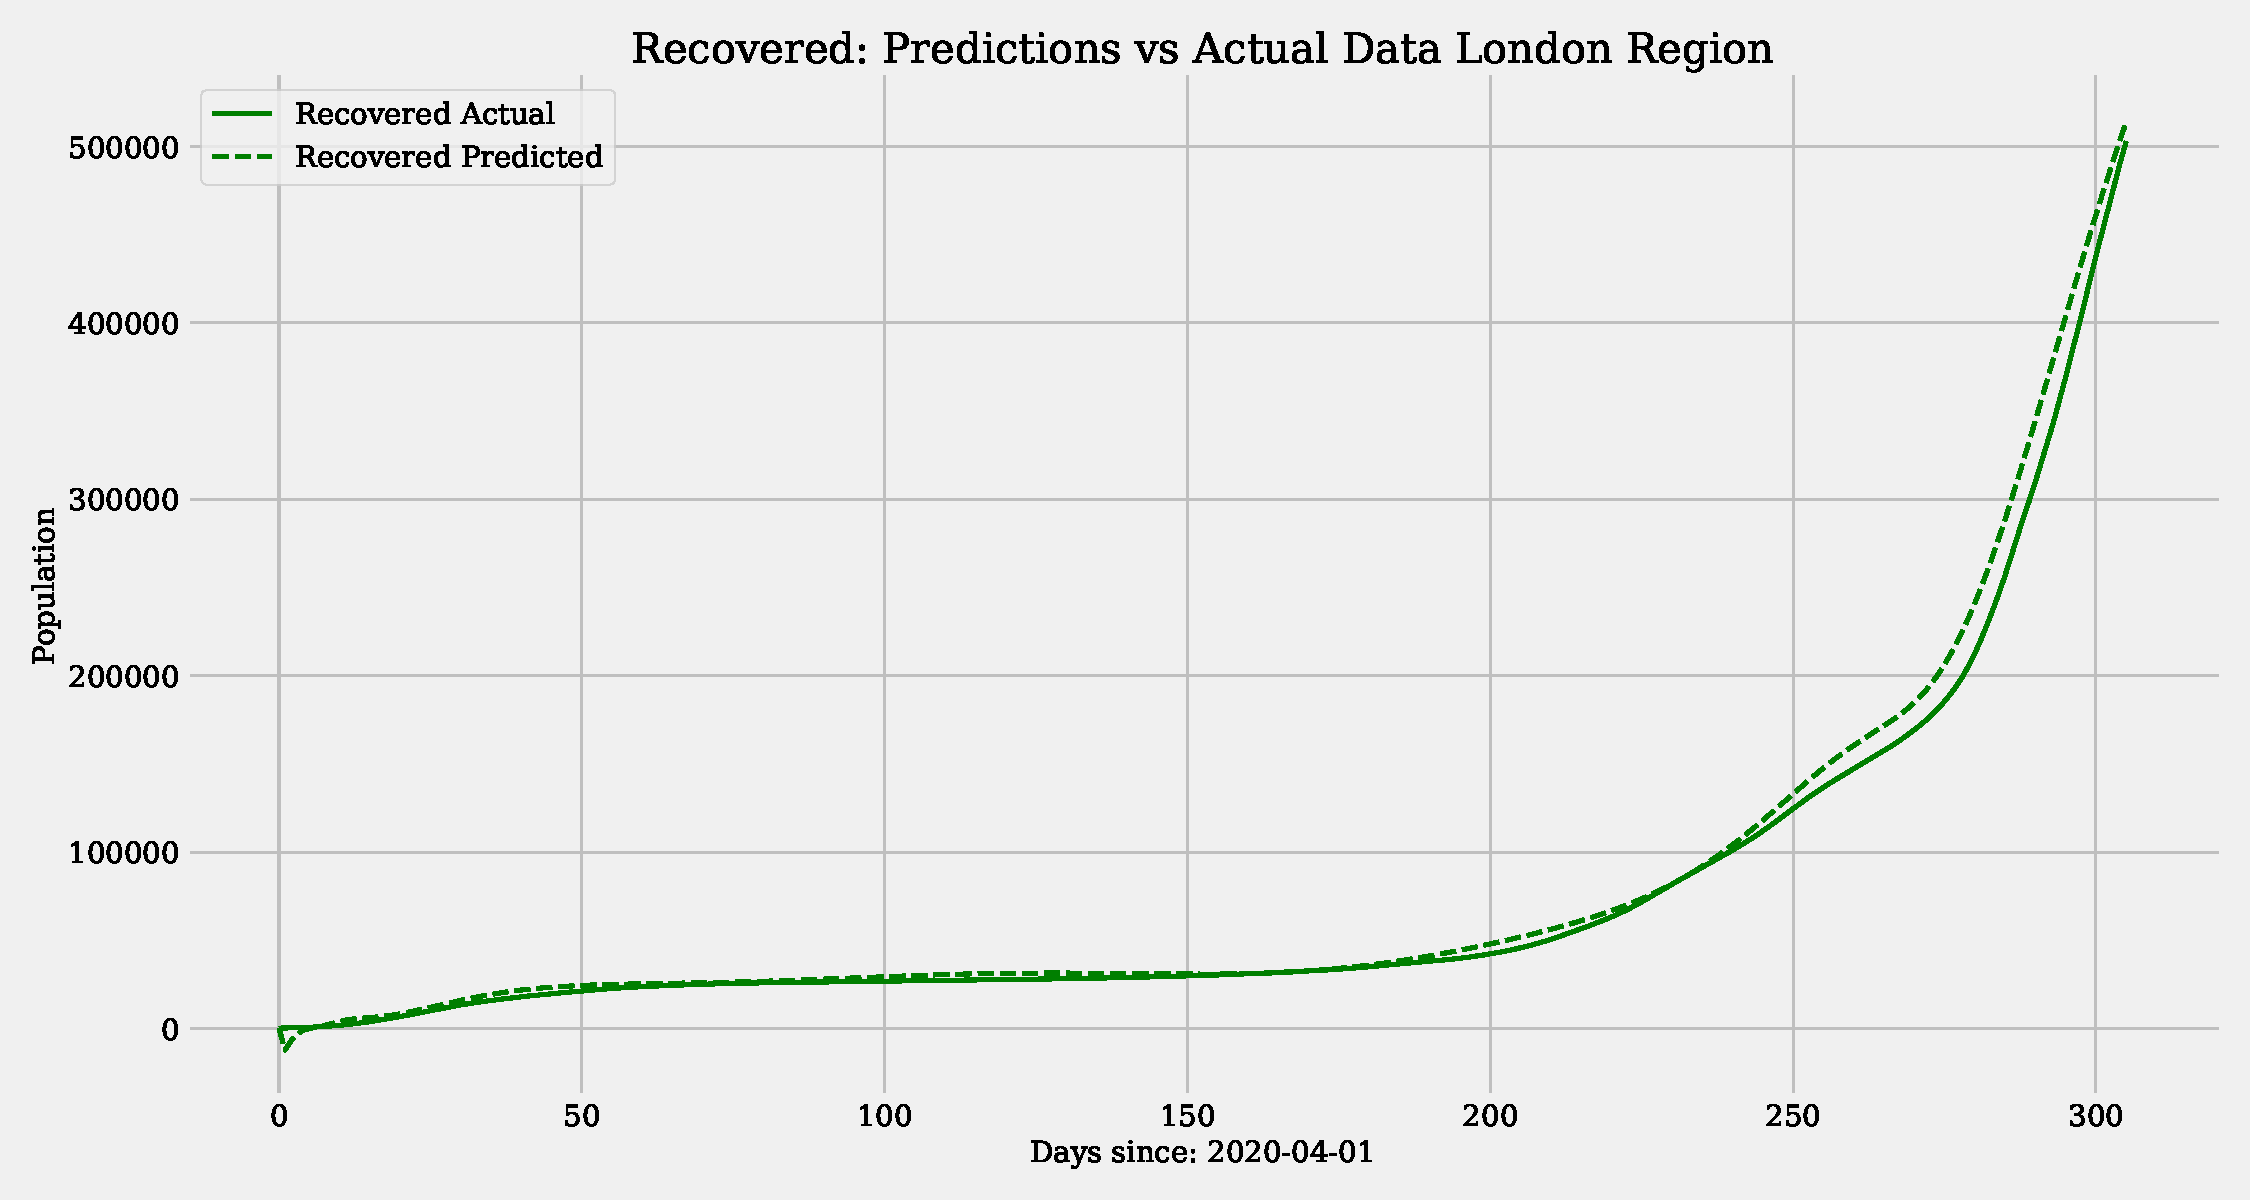
\includegraphics[width=\textwidth]{images/pinn/R_predictions_London Region.pdf}
        \caption{Predicted number of recovered individuals}
        \label{fig:R_predictions_London}
    \end{subfigure}
    \hfill % Ensures that the figures are spaced out evenly
    \begin{subfigure}[t]{0.45\textwidth}
        \centering
        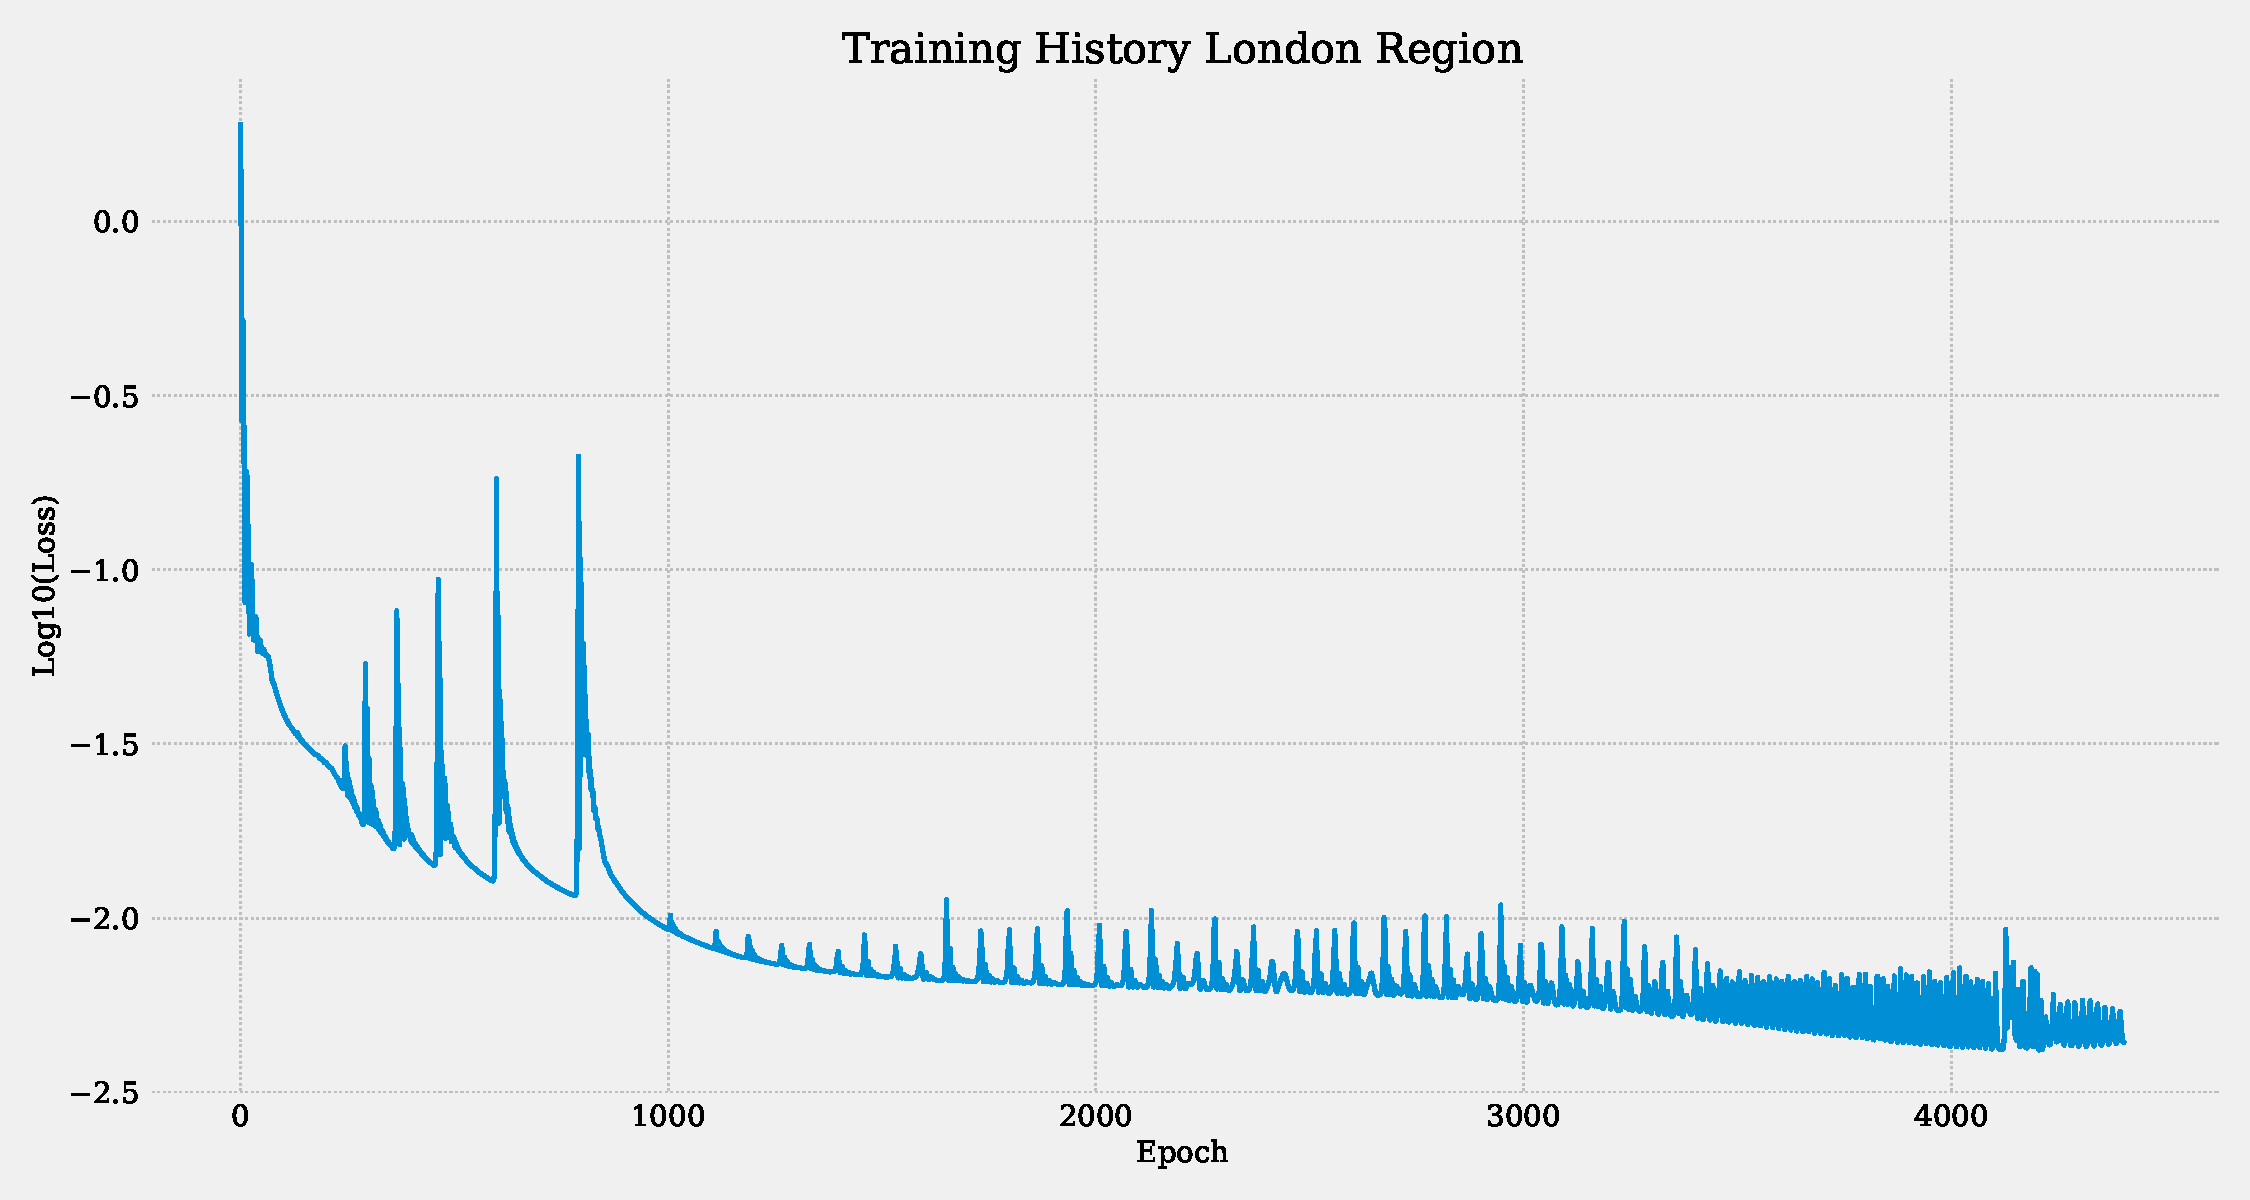
\includegraphics[width=\textwidth]{images/pinn/Training_History_London Region.pdf}
        \caption{Training history of the PINN model}
        \label{fig:Training_History_London}
    \end{subfigure}
    \caption{Physics-Informed Neural Network (PINN) model predictions and training history for the London region, showcasing the dynamics of susceptible, infectious, and recovered populations alongside model training progression.}
    \label{fig:PINN_London_Comprehensive}
\end{figure*}

\begin{figure}[ht]
    \centering
    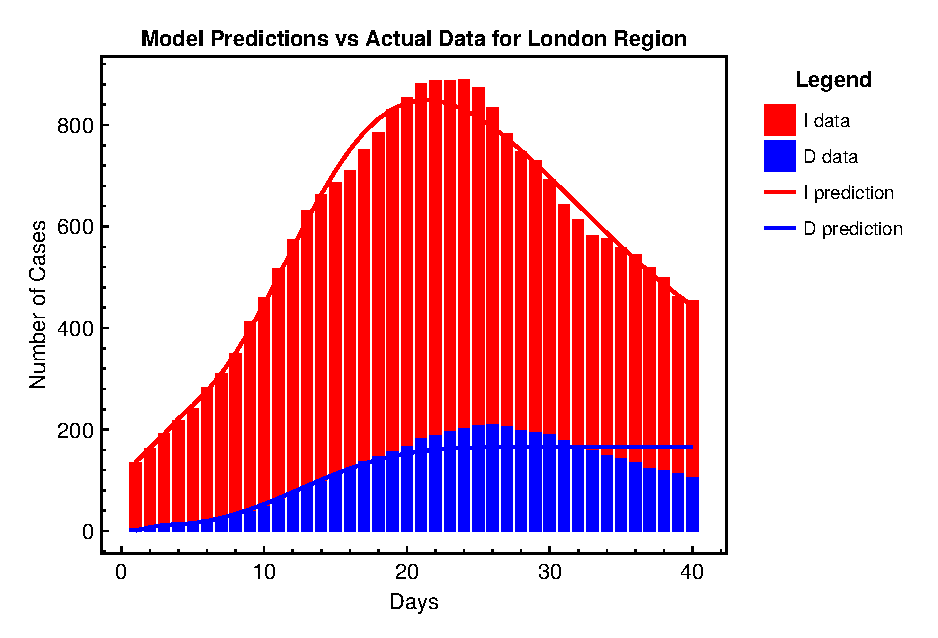
\includegraphics[width=0.8\textwidth]{images/ude/London Region_infected_death_data.pdf}
    \caption{Predicted number of infected and deceased individuals}
    \label{fig:ude_London}
\end{figure}

\subsubsection{Comparison of PINN and UDE Models}
\begin{table}[h!]
    \centering
    \caption{Comparison of PINN and UDE Models Across NHS Regions}
    \label{tab:comparison_results}
    \begin{tabular}{|c|c|c|c|c|}
    \hline
    \textbf{Region} & \textbf{Model} & \textbf{Prediction Type} & \textbf{MAE} & \textbf{RMSE} \\
    \hline
    \multirow{East Midland} & PINN & Infected & 1667.4842 & 2940.2779 \\
    \cline{2-5}
                              & PINN & Deaths & 3687.0097 & 4740.4266 \\
    \cline{2-5}
                              & UDE & Infected & 5.7472 & 1.6529 \\
    \cline{2-5}
                              & UDE & Deaths & 8.2073 & 2.3578 \\
    \hline
    \multirow{East of England} & PINN & Infected & 3583.8807 & 6745.1583 \\
    \cline{2-5}
                              & PINN & Deaths & 4846.2730 & 7033.0405 \\
    \cline{2-5}
                              & UDE & Infected & 9.0658 & 14.4417 \\
    \cline{2-5}
                              & UDE & Deaths & 1.3609 & 2.2810 \\
    \hline
    % Repeat for Regions 3 to 7
    \multirow{London} & PINN & Infected & 5725.1872 & 12032.9975 \\
    \cline{2-5}
                              & PINN & Deaths & 5946.5964 & 10320.4091 \\
    \cline{2-5}
                              & UDE & Infected & 17.1317 & 23.7505 \\
    \cline{2-5}
                              & UDE & Deaths & 17.5006 & 24.9575 \\
    \hline
    
    \multirow{North East England} & PINN & Infected & 1304.2393 & 1944.5151 \\
    \cline{2-5}
                              & PINN & Deaths & 2278.9067 & 3013.1276 \\
    \cline{2-5}
                              & UDE & Infected & 11.4483 & 15.1217 \\
    \cline{2-5}
                              & UDE & Deaths & 2.5449 & 3.3425 \\
    \hline
    
    \multirow{North West England} & PINN & Infected & 5281.3856 & 8504.8463 \\
    \cline{2-5}
                              & PINN & Deaths & 5434.115 & 7574.7920 \\
    \cline{2-5}
                              & UDE & Infected & 20.7050 & 30.8553 \\
    \cline{2-5}
                              & UDE & Deaths & 3.4221 & 5.6294 \\
    \hline
    
    \multirow{South East England} & PINN & Infected & 3924.1983 & 8271.0872 \\
    \cline{2-5}
                              & PINN & Deaths & 4148.2084 & 7579.5345 \\
    \cline{2-5}
                              & UDE & Infected & 7.3596 & 11.0826 \\
    \cline{2-5}
                              & UDE & Deaths & 1.8857 & 3.4590 \\
    \hline
    
    \multirow{South West England} & PINN & Infected & 1299.2248 & 2409.3609 \\
    \cline{2-5}
                              & PINN & Deaths & 2179.7401 & 2299.8993 \\
    \cline{2-5}
                              & UDE & Infected & 4.0182 & 5.07486 \\
    \cline{2-5}
                              & UDE & Deaths & 1.3279 & 1.8393 \\
    \hline
    
    \multirow{West midlands} & PINN & Infected & 2491.6001 & 4394.4118 \\
    \cline{2-5}
                              & PINN & Deaths & 3362.2455 & 5750.7348 \\
    \cline{2-5}
                              & UDE & Infected & 7.9585 & 10.4482 \\
    \cline{2-5}
                              & UDE & Deaths & 4.4496 & 6.4756 \\
    \hline
    \multirow{Yorkshire and the Humber} & PINN & Infected & 2396.9159 & 4023.9809 \\
    \cline{2-5}
                              & PINN & Deaths & 3152.3625 & 4207.7251 \\
    \cline{2-5}
                              & UDE & Infected & 4.8312 & 6.4747 \\
    \cline{2-5}
                              & UDE & Deaths & 1.0738 & 1.6862 \\
    \hline
    \end{tabular}
    \end{table}
    

\section{Conclusion}





\begin{figure*}[h]
    \centering
    \begin{subfigure}[t]{0.45\textwidth}
        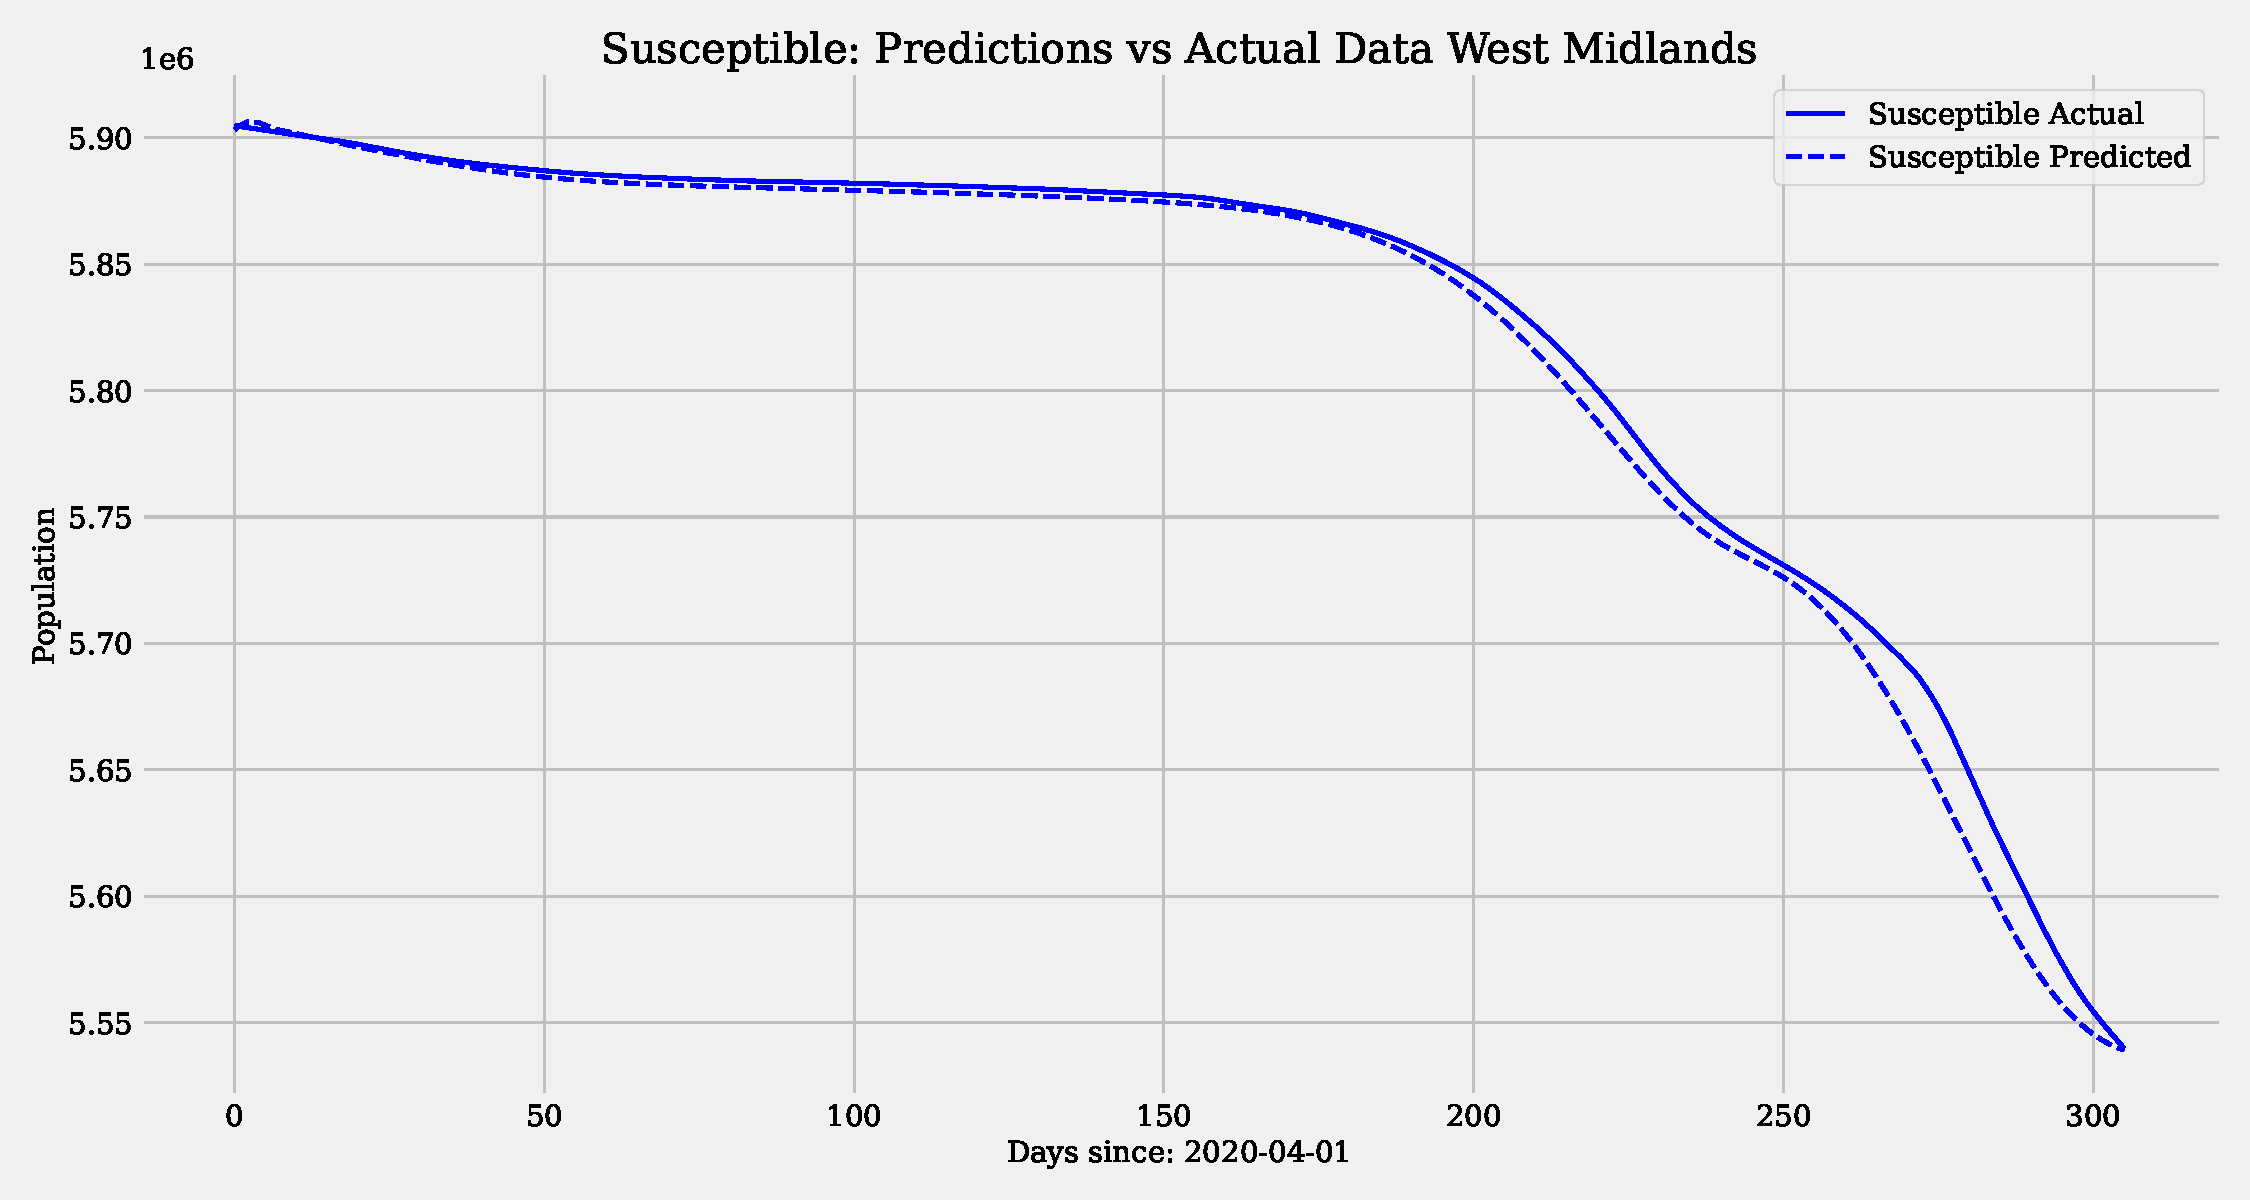
\includegraphics[width=\textwidth]{images/pinn/S_predictions_West Midlands.pdf}
        \caption{Predicted number of susceptible individuals}
        \label{fig:S_predictions_West Midlands}
    \end{subfigure}
    \hfill % Ensures that the figures are spaced out evenly
    \begin{subfigure}[t]{0.45\textwidth}
        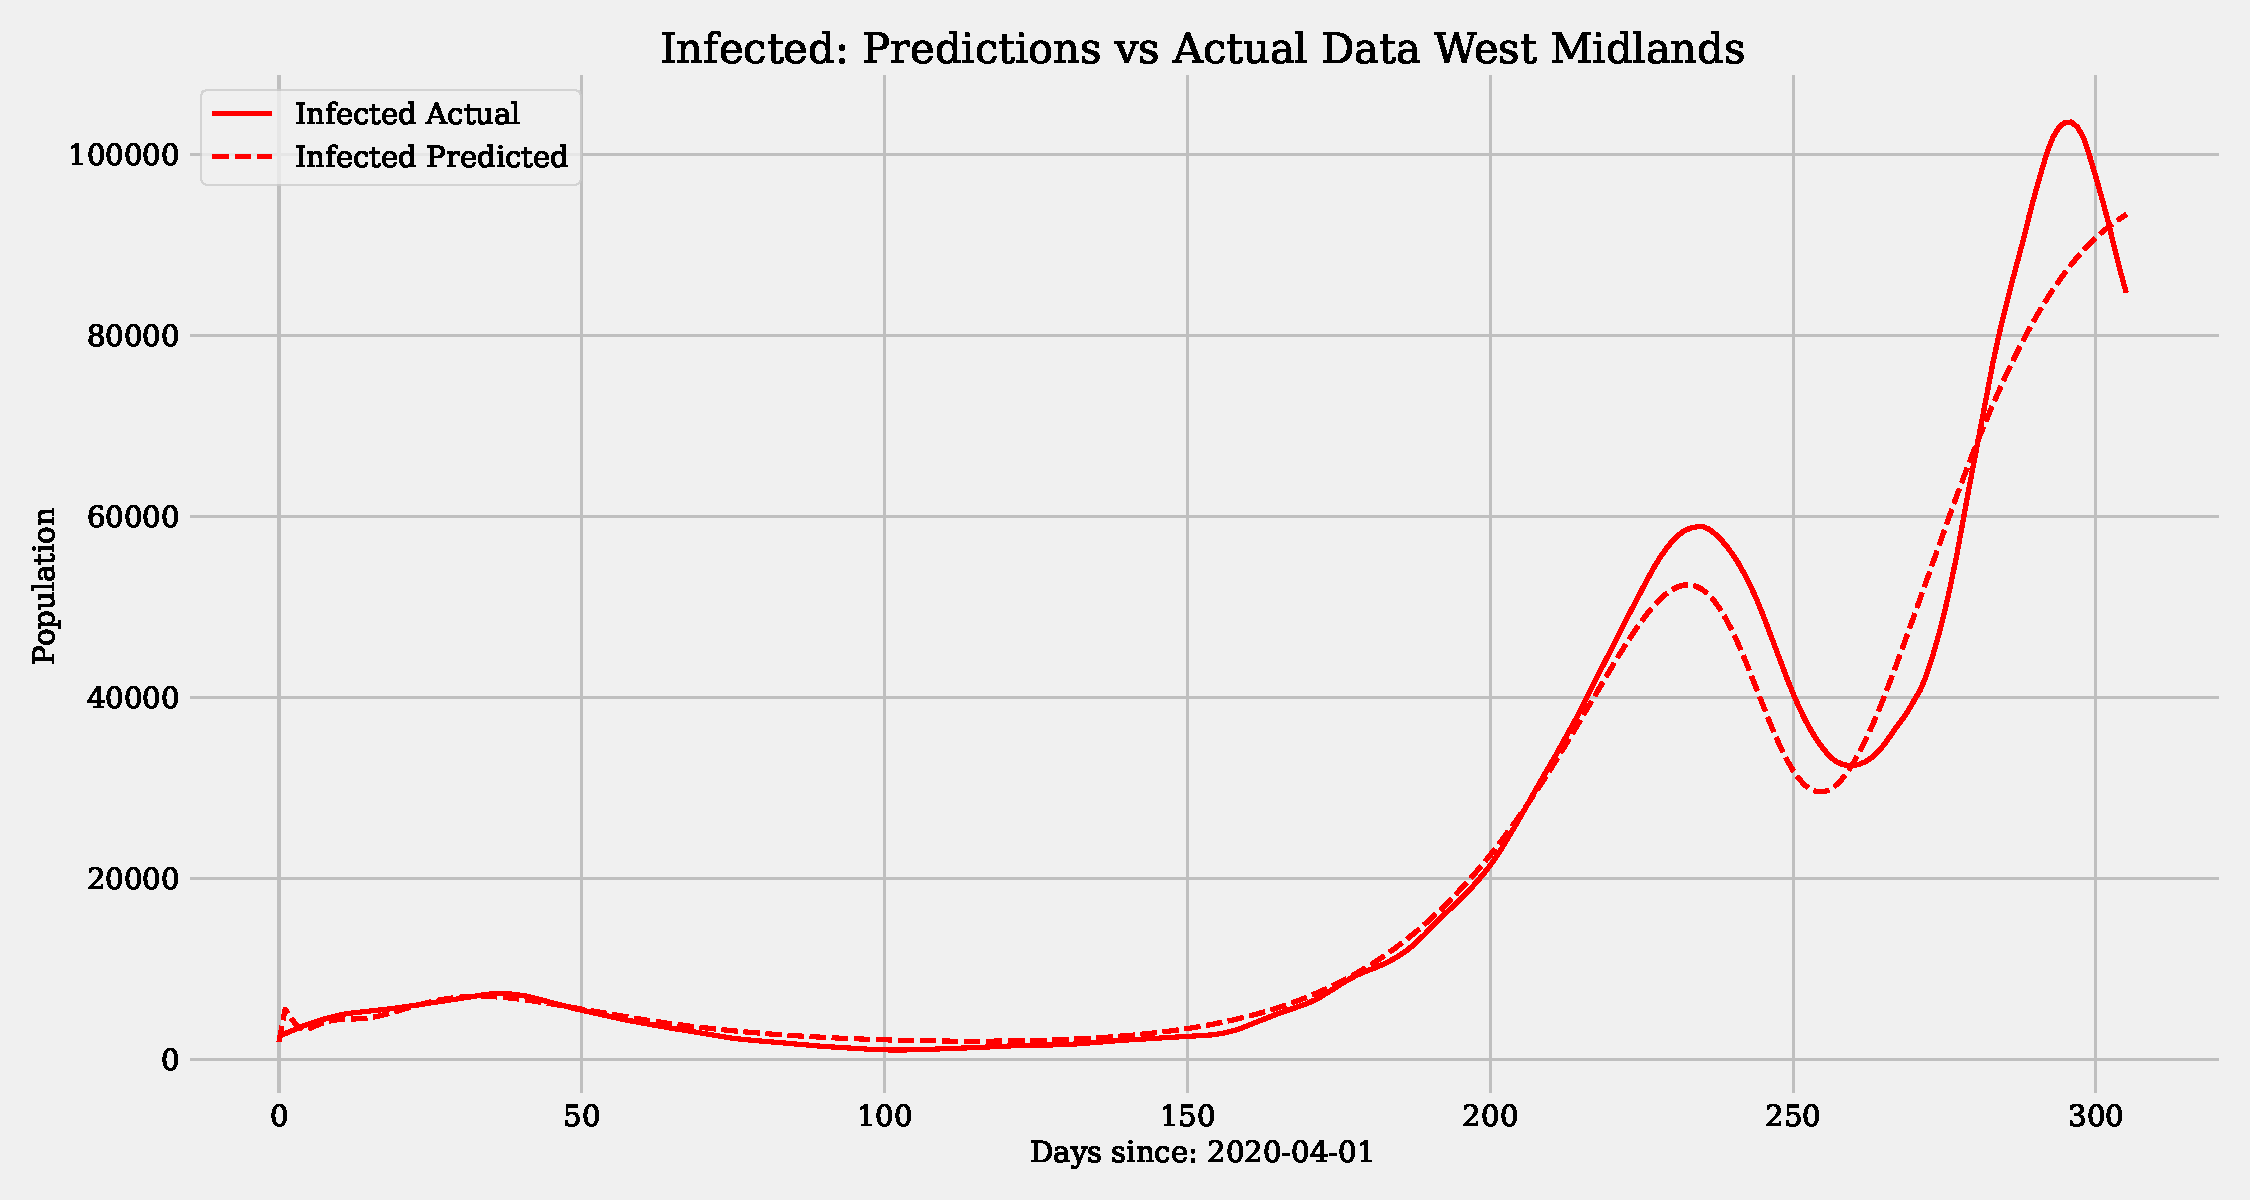
\includegraphics[width=\textwidth]{images/pinn/I_predictions_West Midlands.pdf}
        \caption{Predicted number of infectious individuals}
        \label{fig:I_predictions_West Midlands}
    \end{subfigure}

    % Adds a bit of vertical space between the rows of figures
    \vspace{0.5cm}

    \begin{subfigure}[t]{0.45\textwidth}
        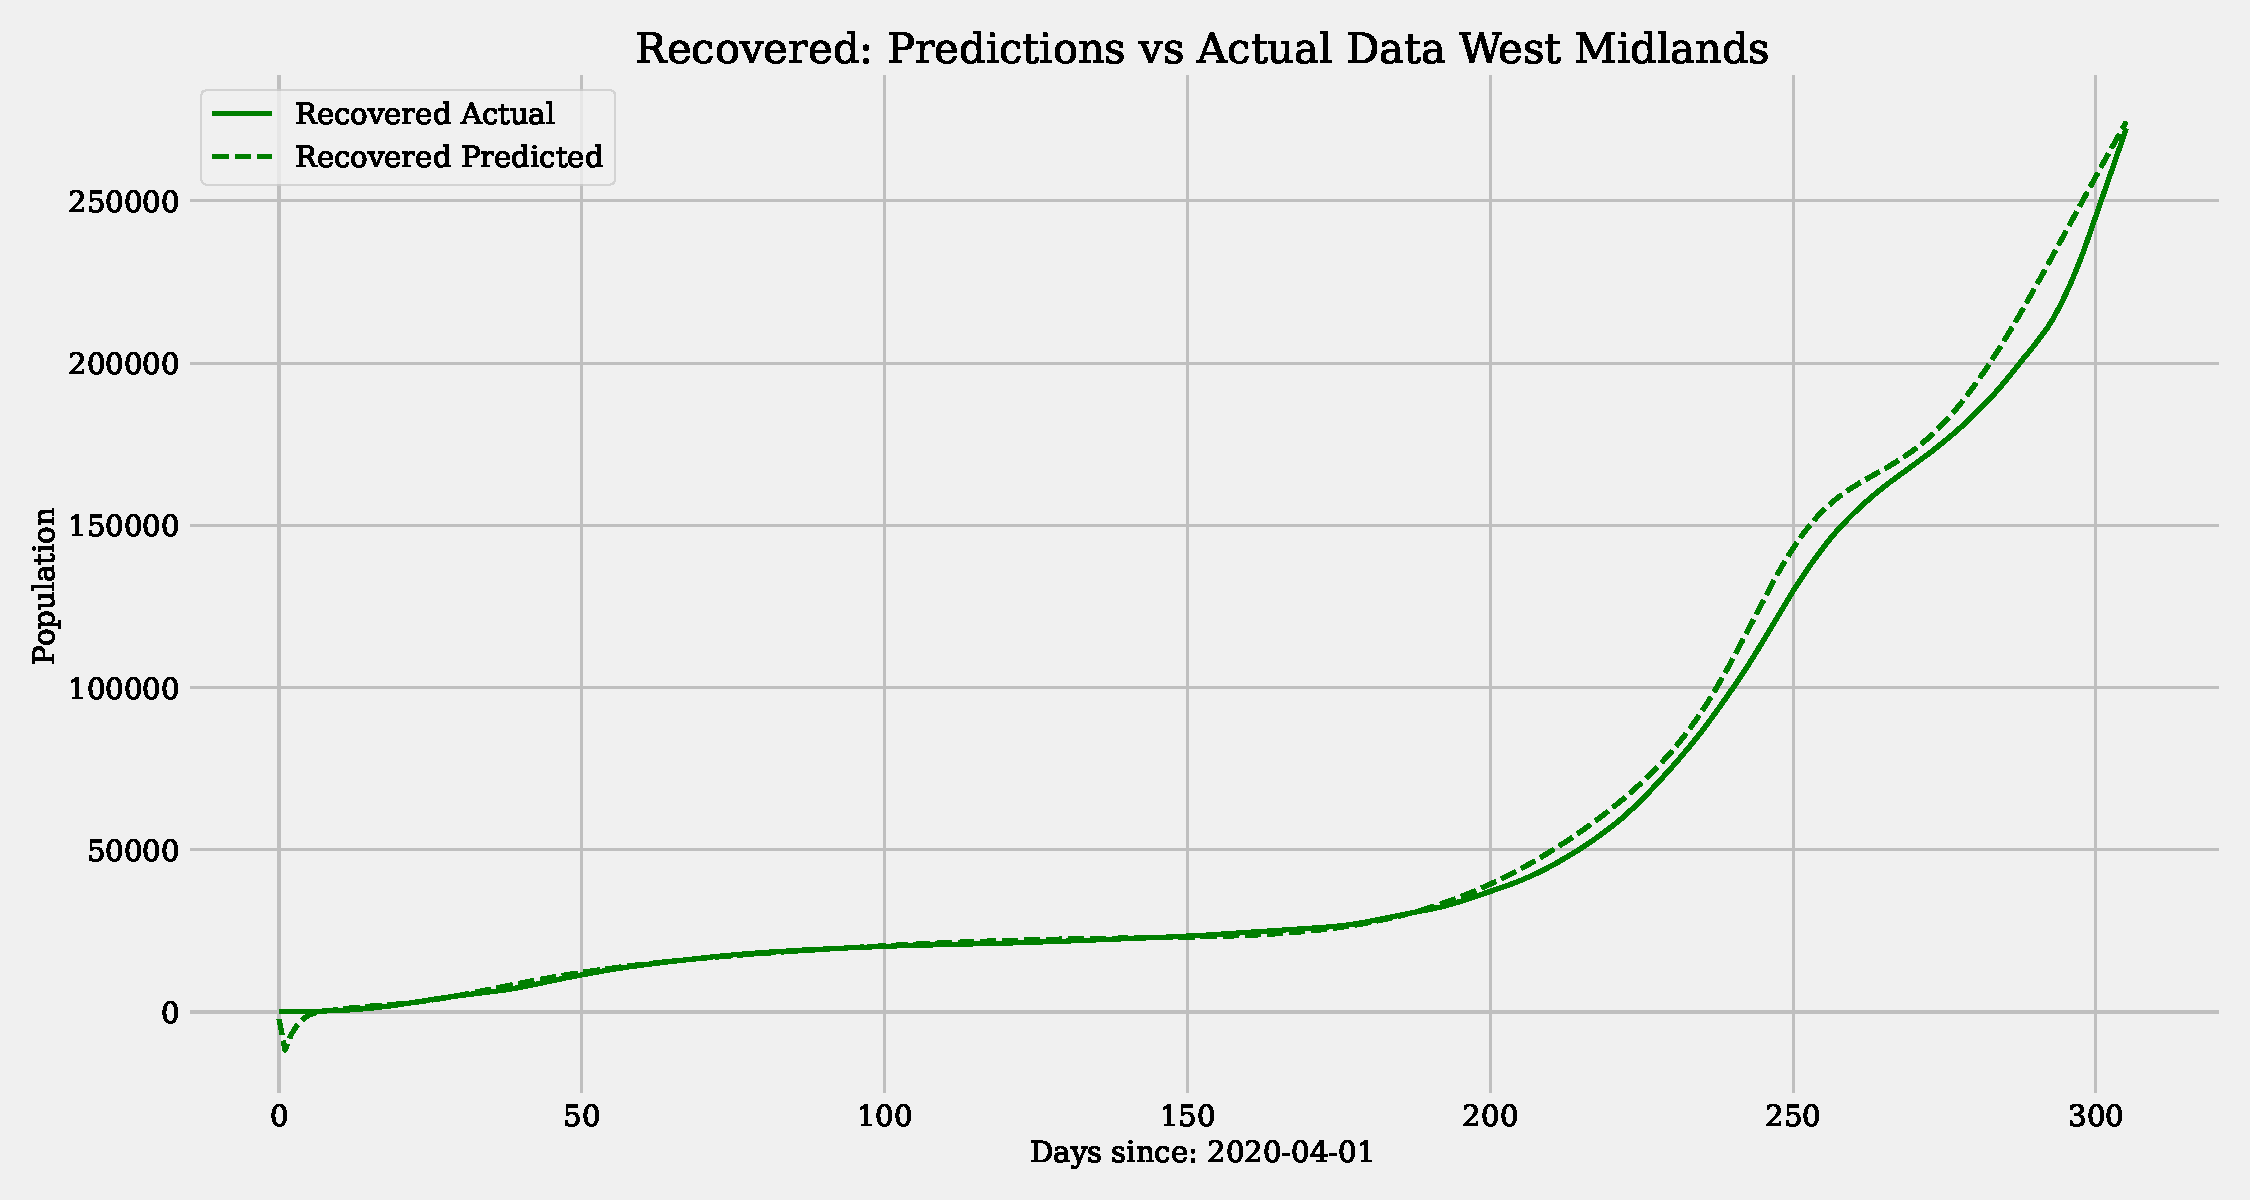
\includegraphics[width=\textwidth]{images/pinn/R_predictions_West Midlands.pdf}
        \caption{Predicted number of recovered individuals}
        \label{fig:R_predictions_West Midlands}
    \end{subfigure}
    \hfill % Ensures that the figures are spaced out evenly
    \begin{subfigure}[t]{0.45\textwidth}
        \centering
        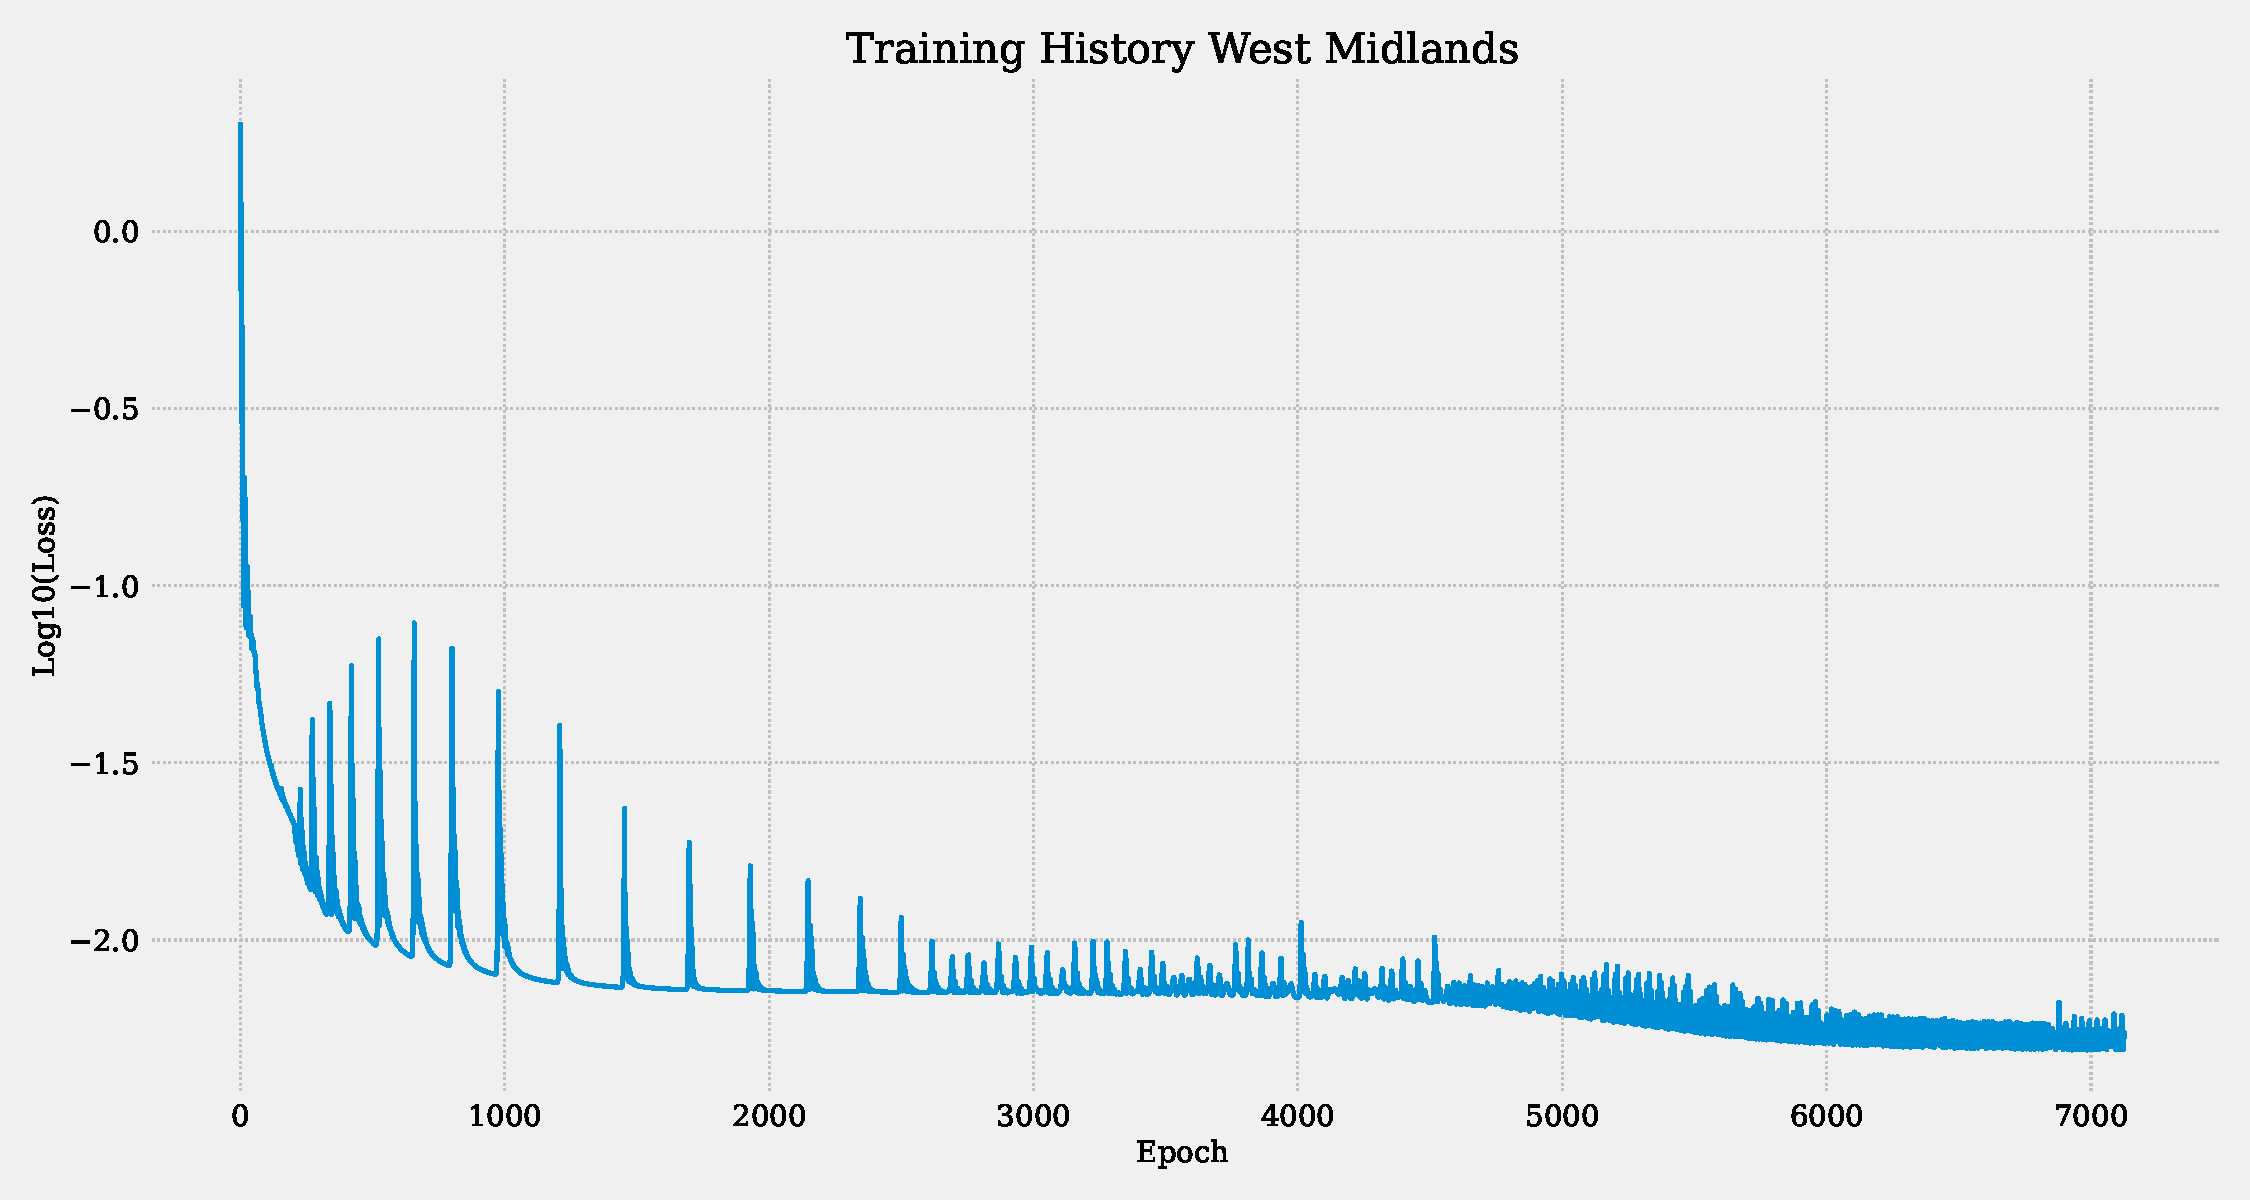
\includegraphics[width=\textwidth]{images/pinn/Training_History_West Midlands.pdf}
        \caption{Training history of the PINN model}
        \label{fig:Training_History_West Midlands}
    \end{subfigure}
    \caption{Physics-Informed Neural Network (PINN) model predictions and training history for the West Midlands region, showcasing the dynamics of susceptible, infectious, and recovered populations alongside model training progression.}
    \label{fig:PINN_West Midlands_Comprehensive}
\end{figure*}


\begin{figure}[h]
    \centering
    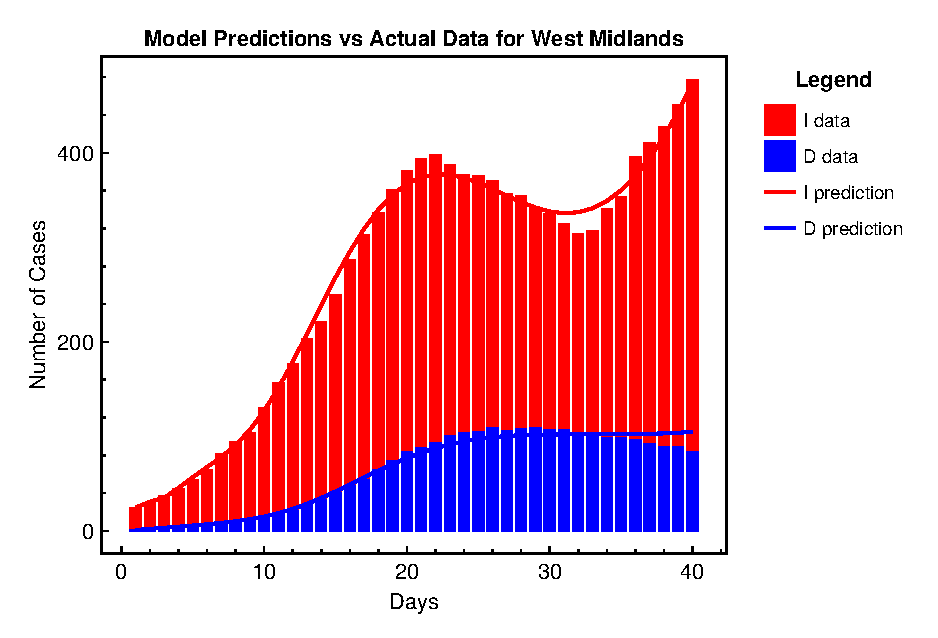
\includegraphics[width=0.8\textwidth]{images/ude/West Midlands_infected_death_data.pdf}
    \caption{Predicted number of infected and deceased individuals}
    \label{fig:ude_West Midlands}
\end{figure}


\begin{figure*}[h]
    \centering
    \begin{subfigure}[t]{0.45\textwidth}
        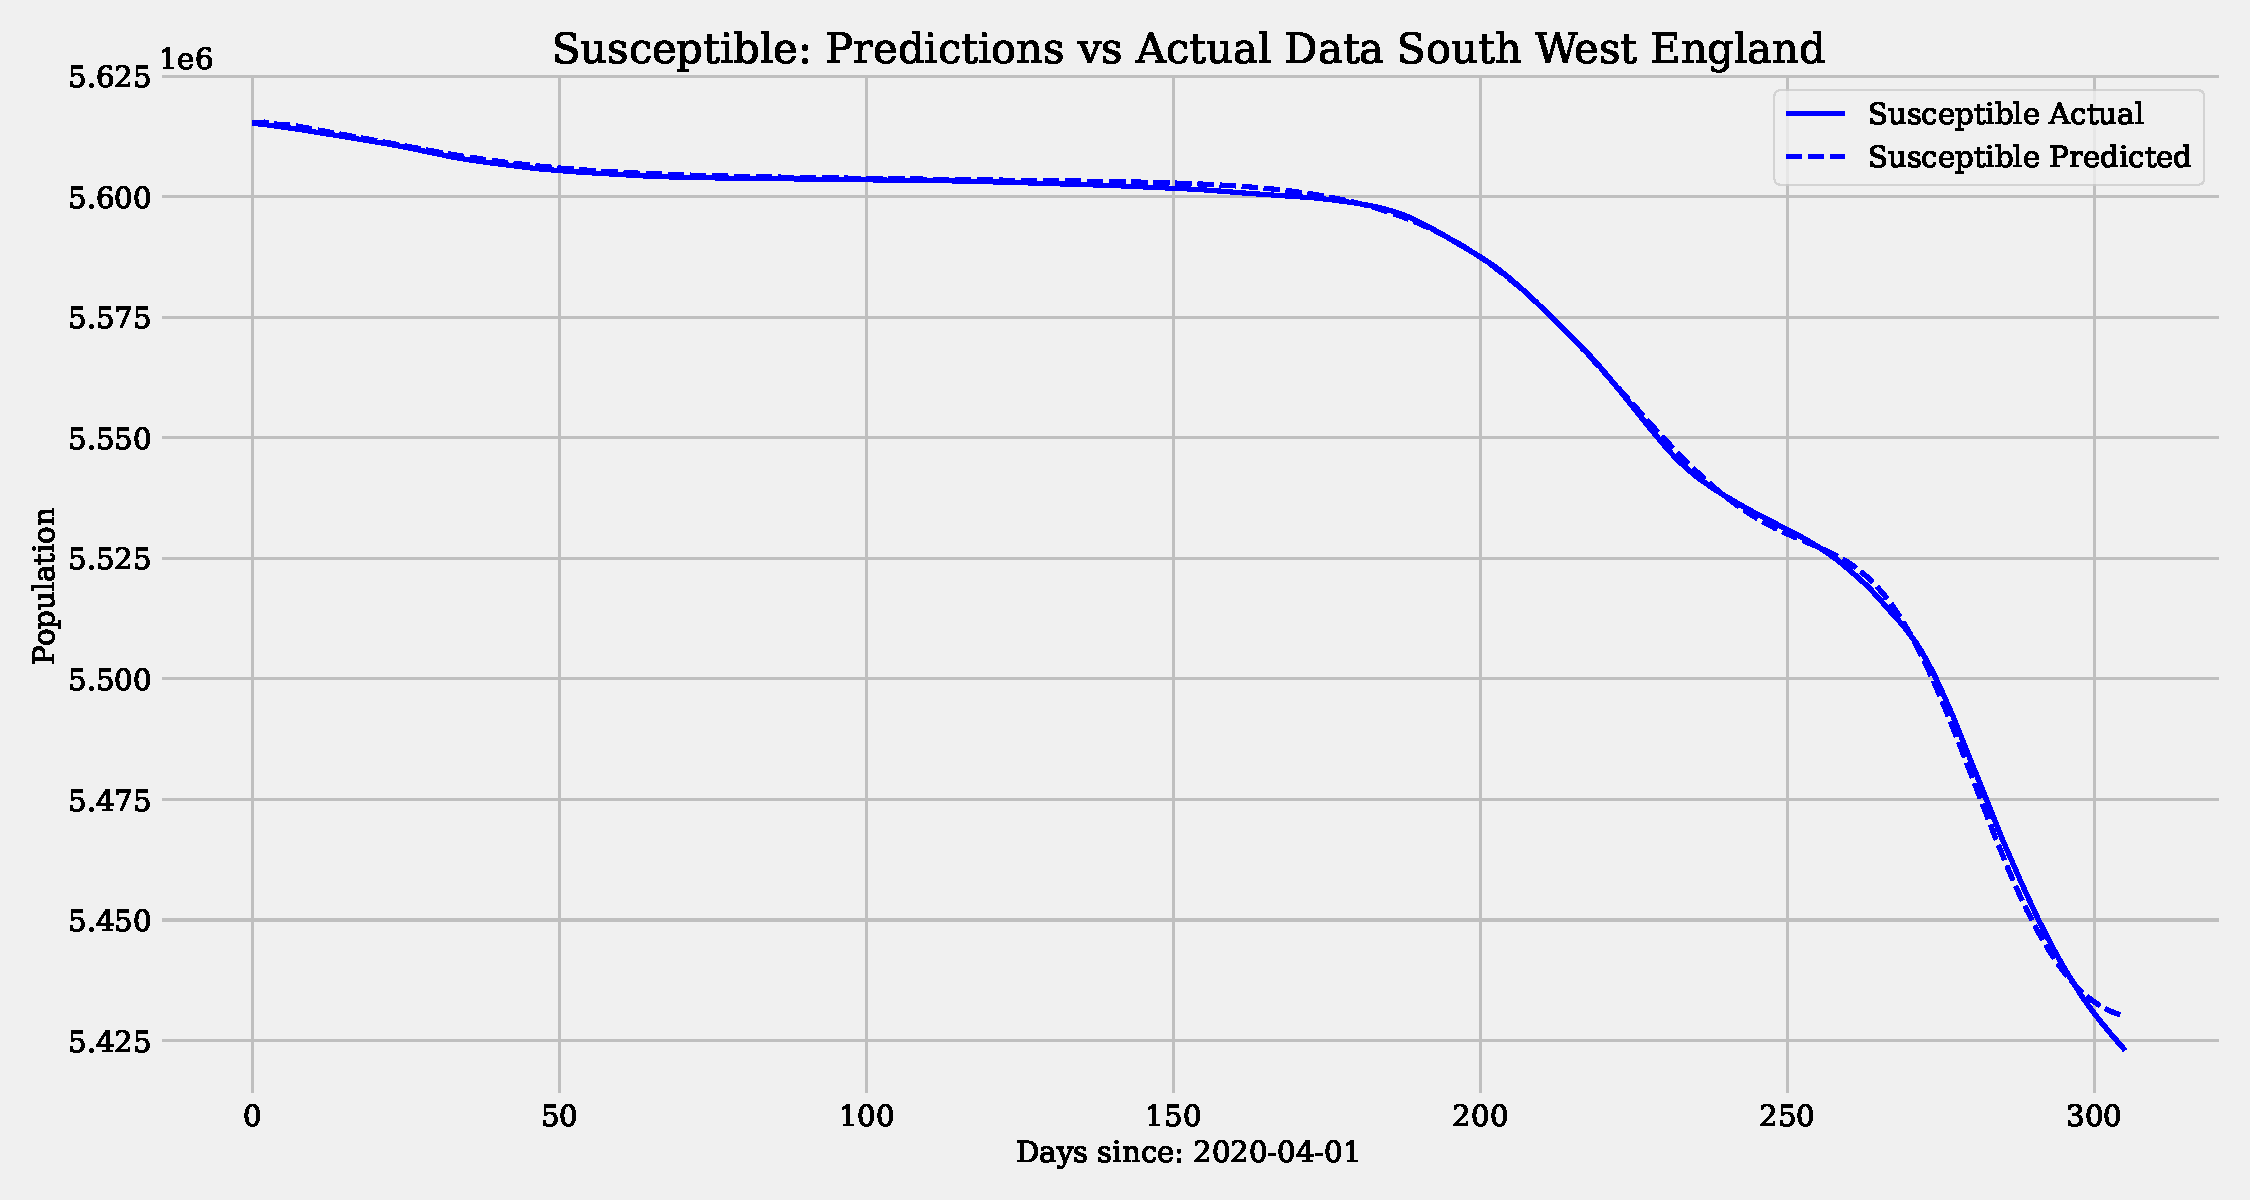
\includegraphics[width=\textwidth]{images/pinn/S_predictions_South West England.pdf}
        \caption{Predicted number of susceptible individuals}
        \label{fig:S_predictions_South West England}
    \end{subfigure}
    \hfill % Ensures that the figures are spaced out evenly
    \begin{subfigure}[t]{0.45\textwidth}
        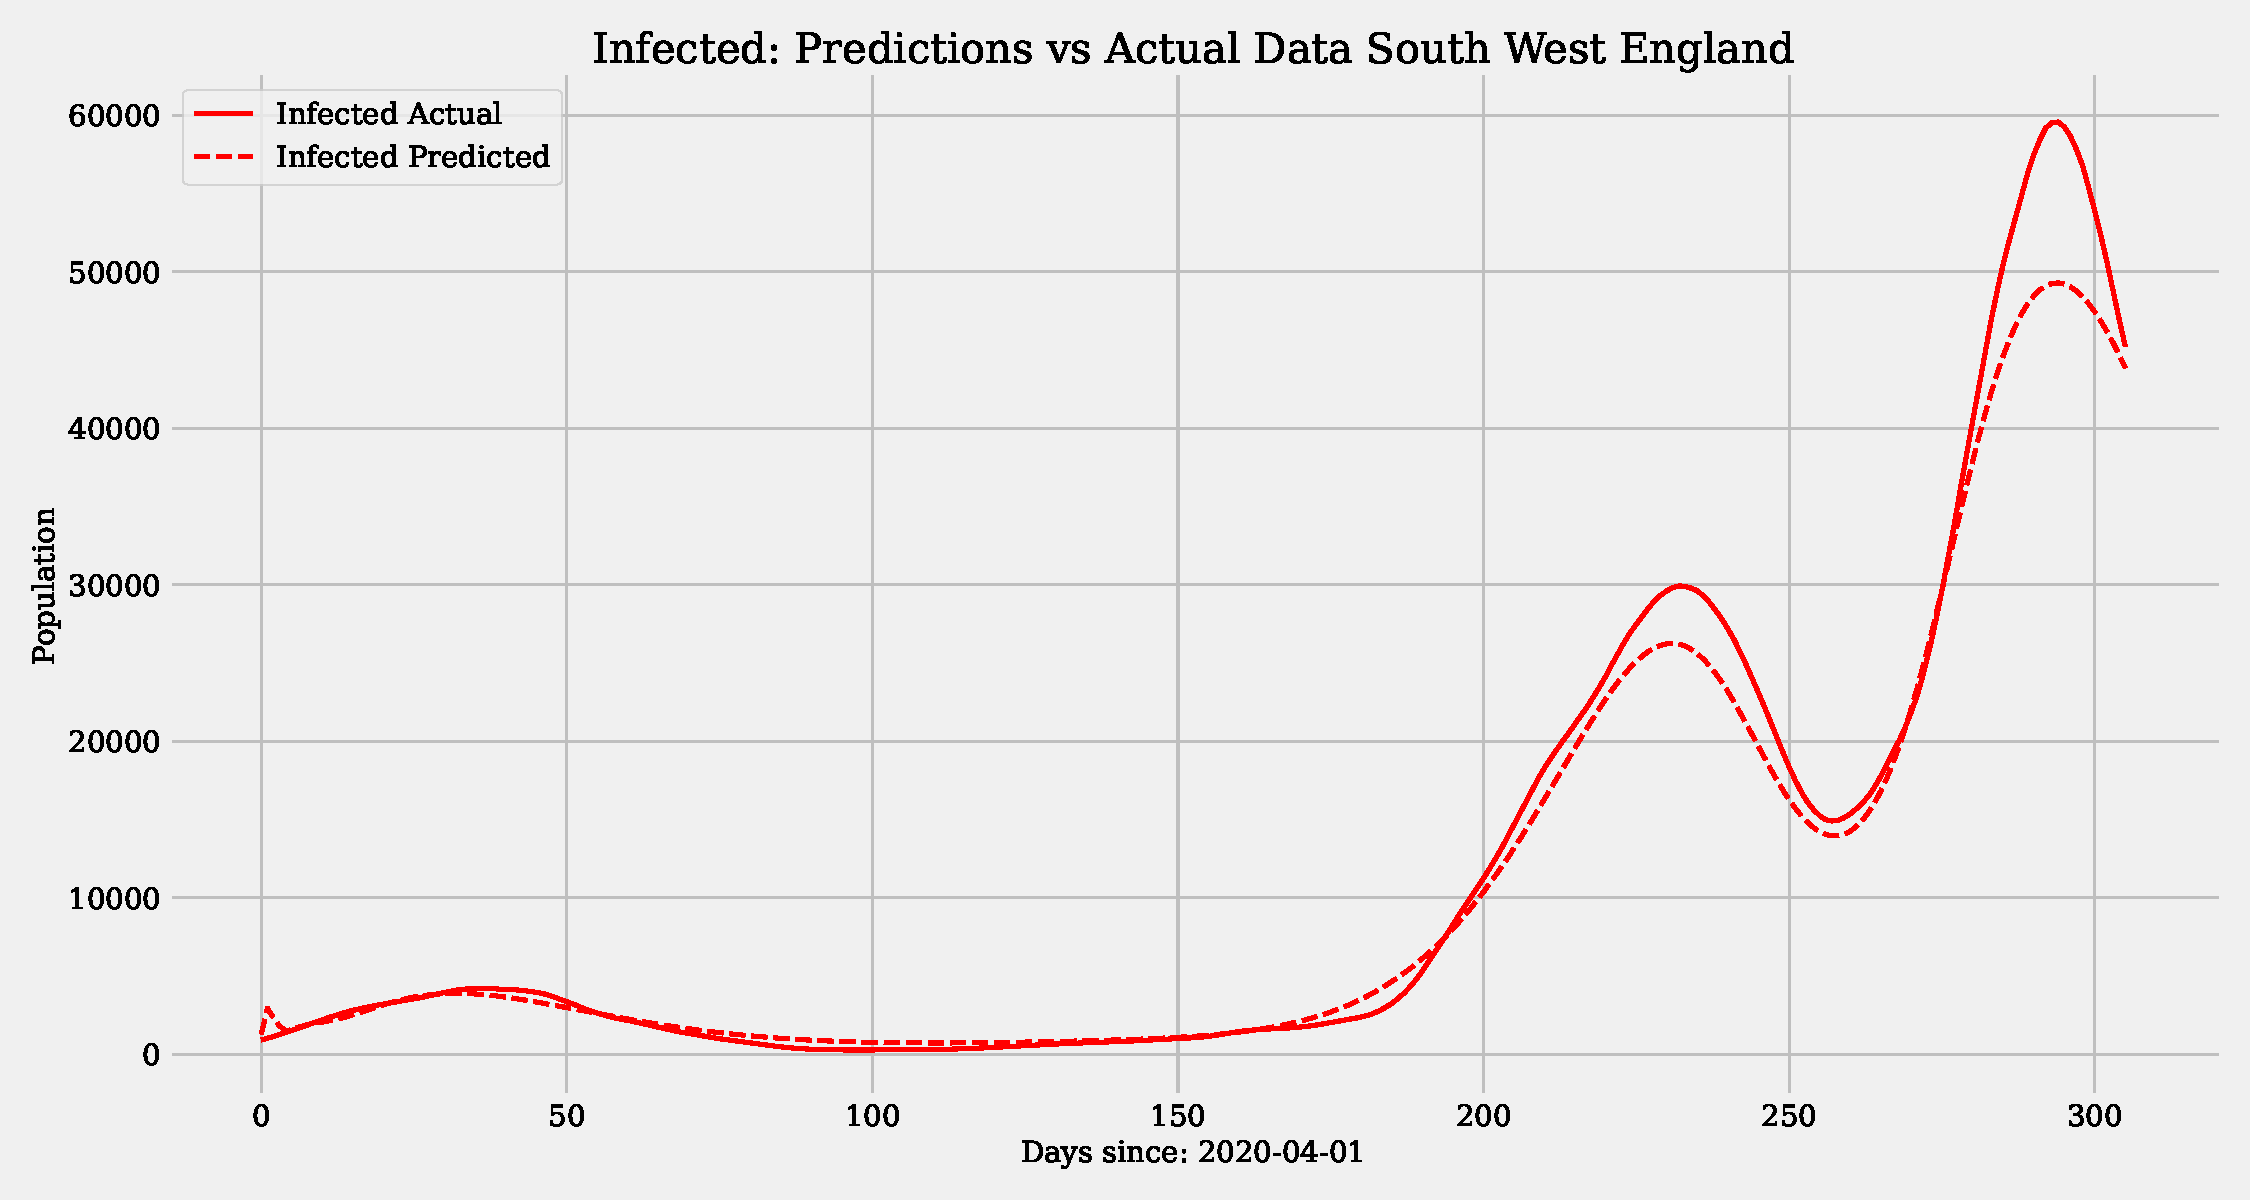
\includegraphics[width=\textwidth]{images/pinn/I_predictions_South West England.pdf}
        \caption{Predicted number of infectious individuals}
        \label{fig:I_predictions_South West England}
    \end{subfigure}

    % Adds a bit of vertical space between the rows of figures
    \vspace{0.5cm}

    \begin{subfigure}[t]{0.45\textwidth}
        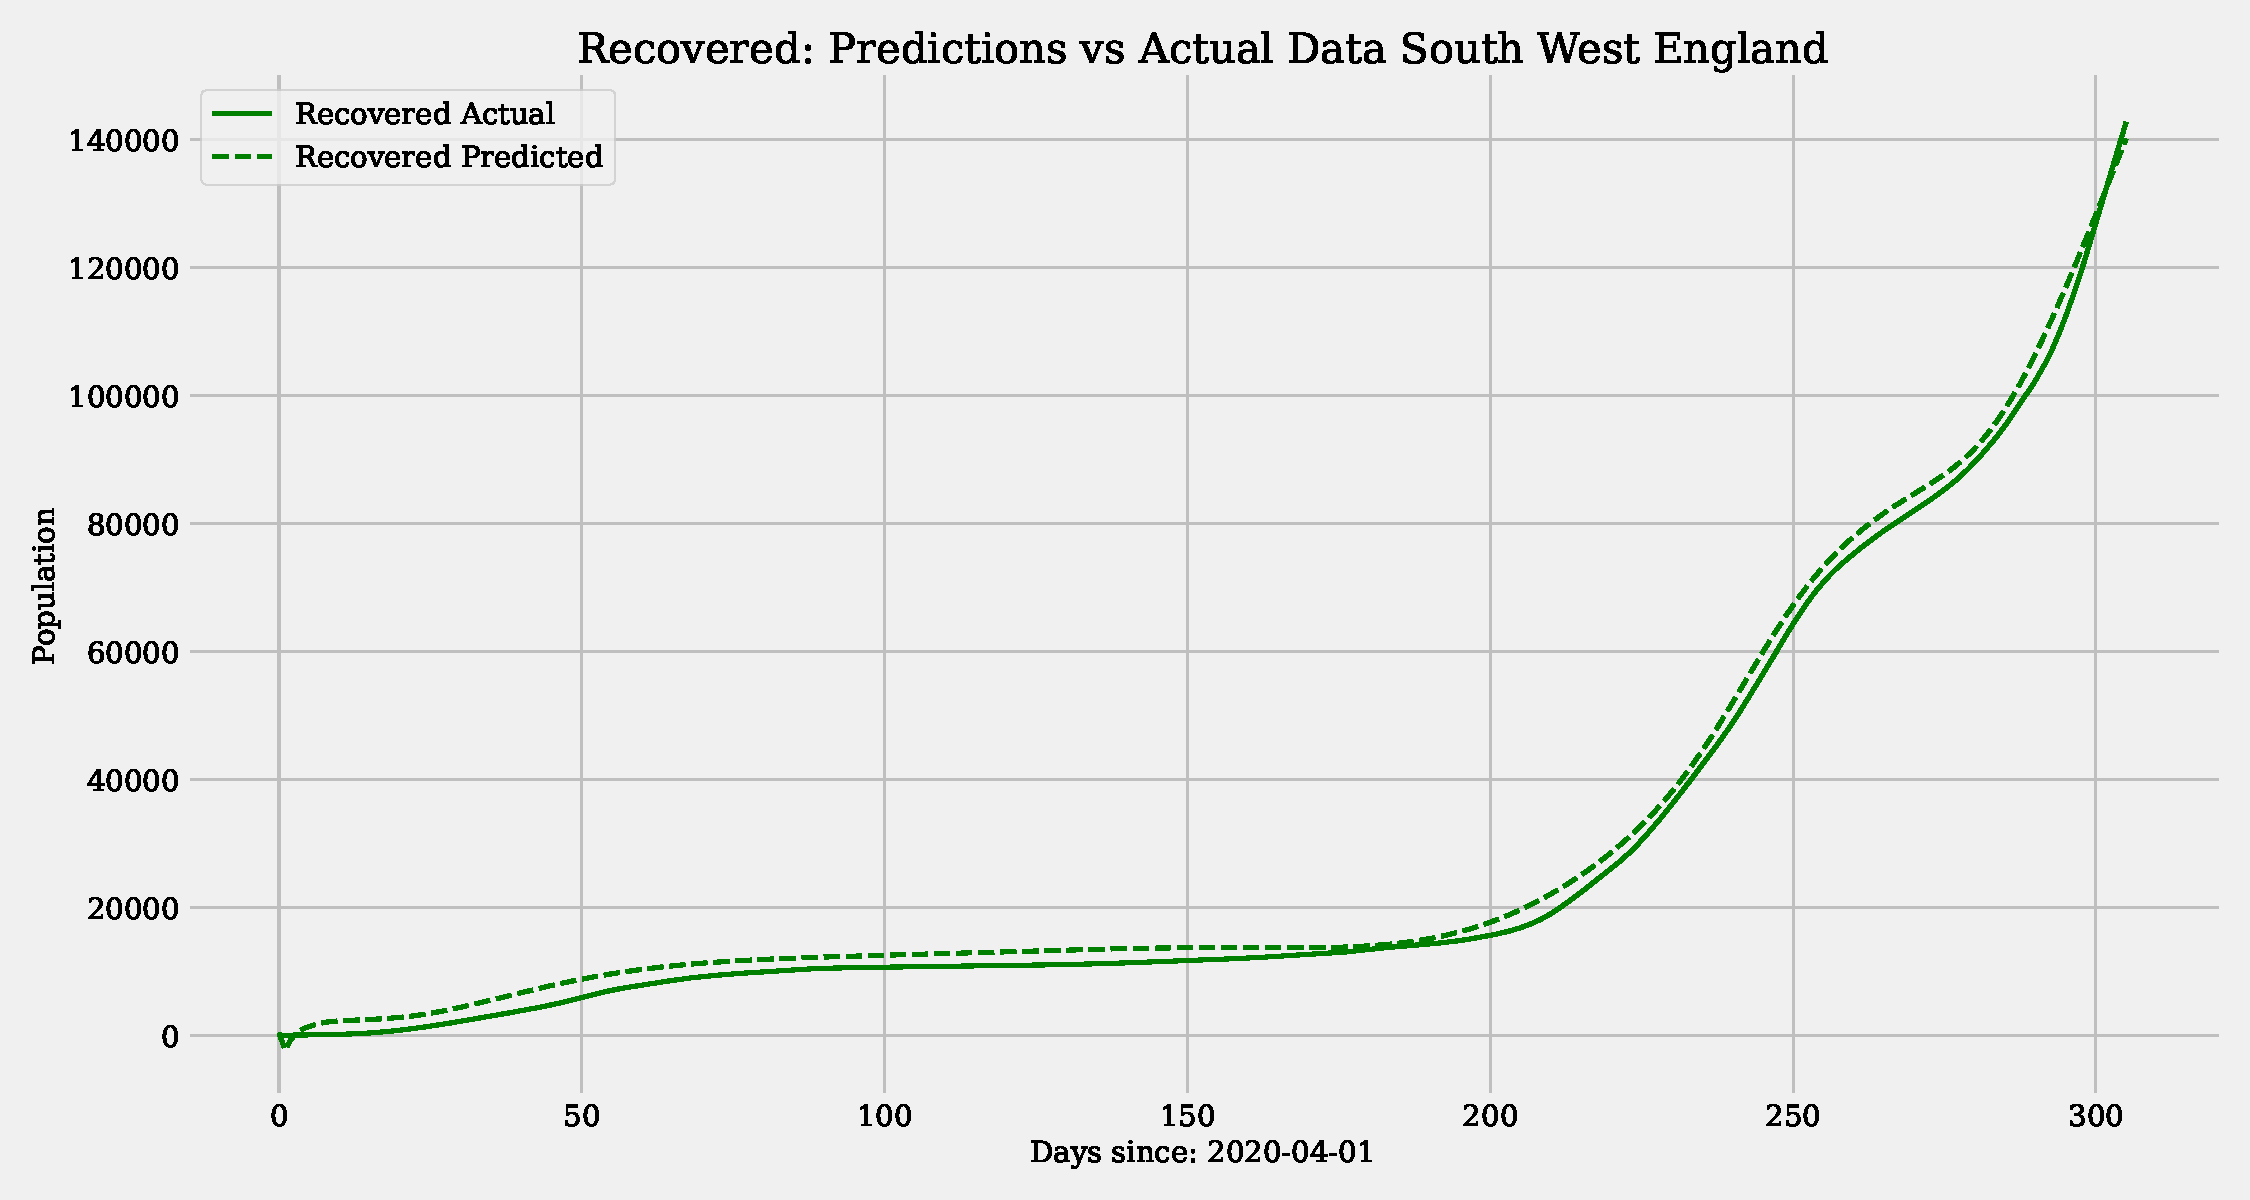
\includegraphics[width=\textwidth]{images/pinn/R_predictions_South West England.pdf}
        \caption{Predicted number of recovered individuals}
        \label{fig:R_predictions_South West England}
    \end{subfigure}
    \hfill % Ensures that the figures are spaced out evenly
    \begin{subfigure}[t]{0.45\textwidth}
        \centering
        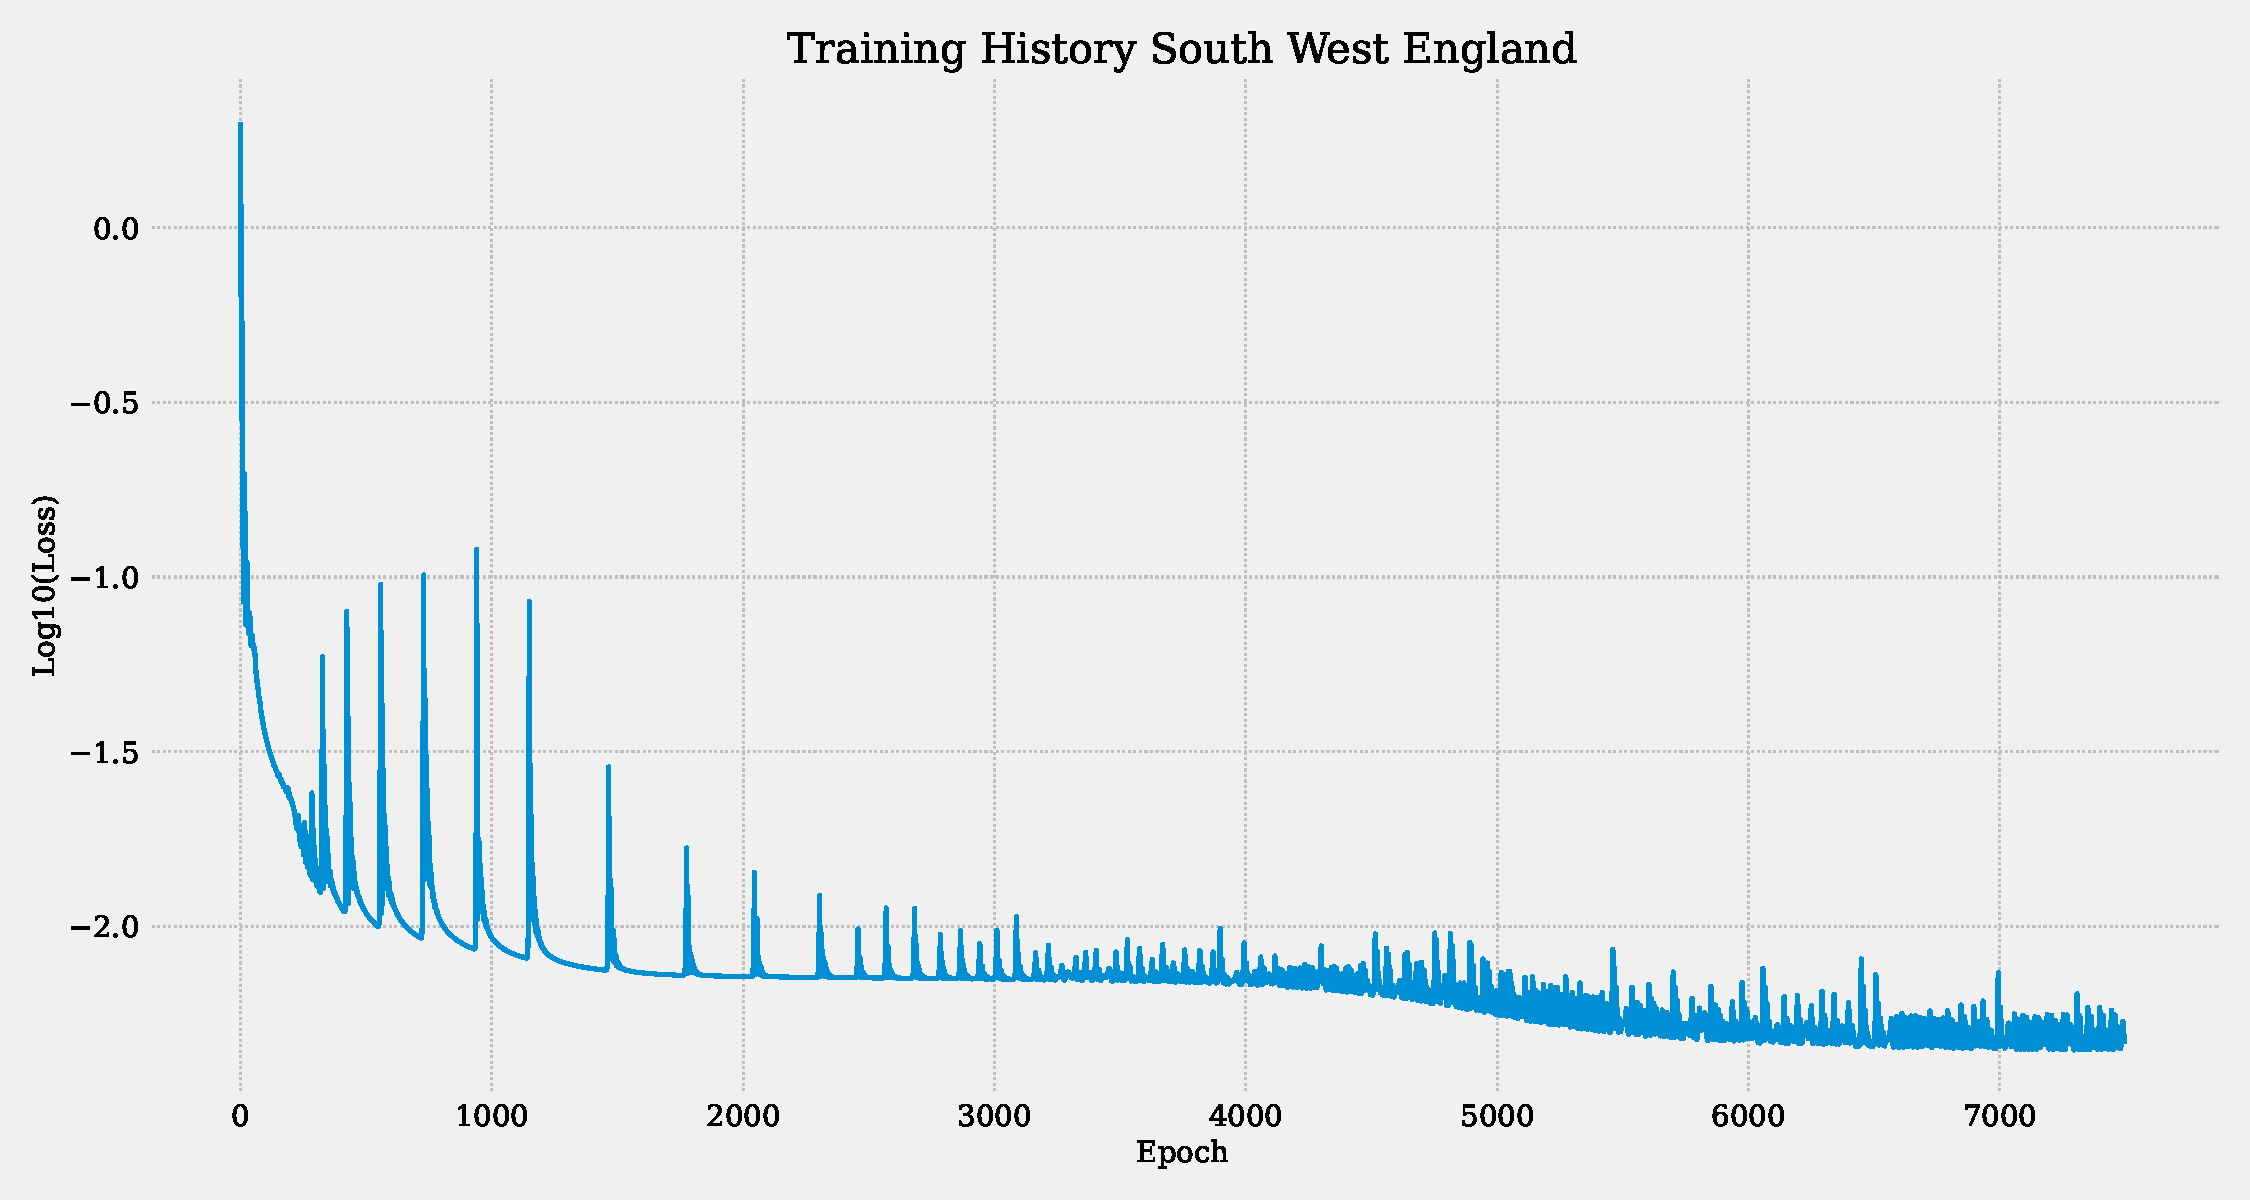
\includegraphics[width=\textwidth]{images/pinn/Training_History_South West England.pdf}
        \caption{Training history of the PINN model}
        \label{fig:Training_History_South West England}
    \end{subfigure}
    \caption{Physics-Informed Neural Network (PINN) model predictions and training history for the South West England region, showcasing the dynamics of susceptible, infectious, and recovered populations alongside model training progression.}
    \label{fig:PINN_South West England_Comprehensive}

\end{figure*}

\begin{figure}[h]
    \centering
    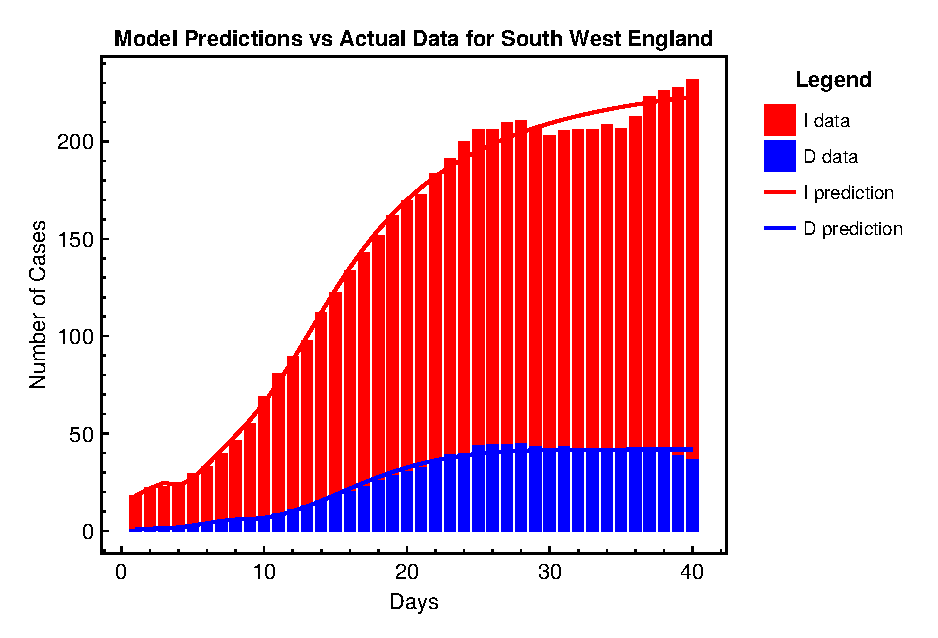
\includegraphics[width=0.8\textwidth]{images/ude/South West England_infected_death_data.pdf}
    \caption{Predicted number of infected and deceased individuals}
    \label{fig:ude_South West England}
\end{figure}


\begin{figure*}
    \centering
    \begin{subfigure}[t]{0.45\textwidth}
        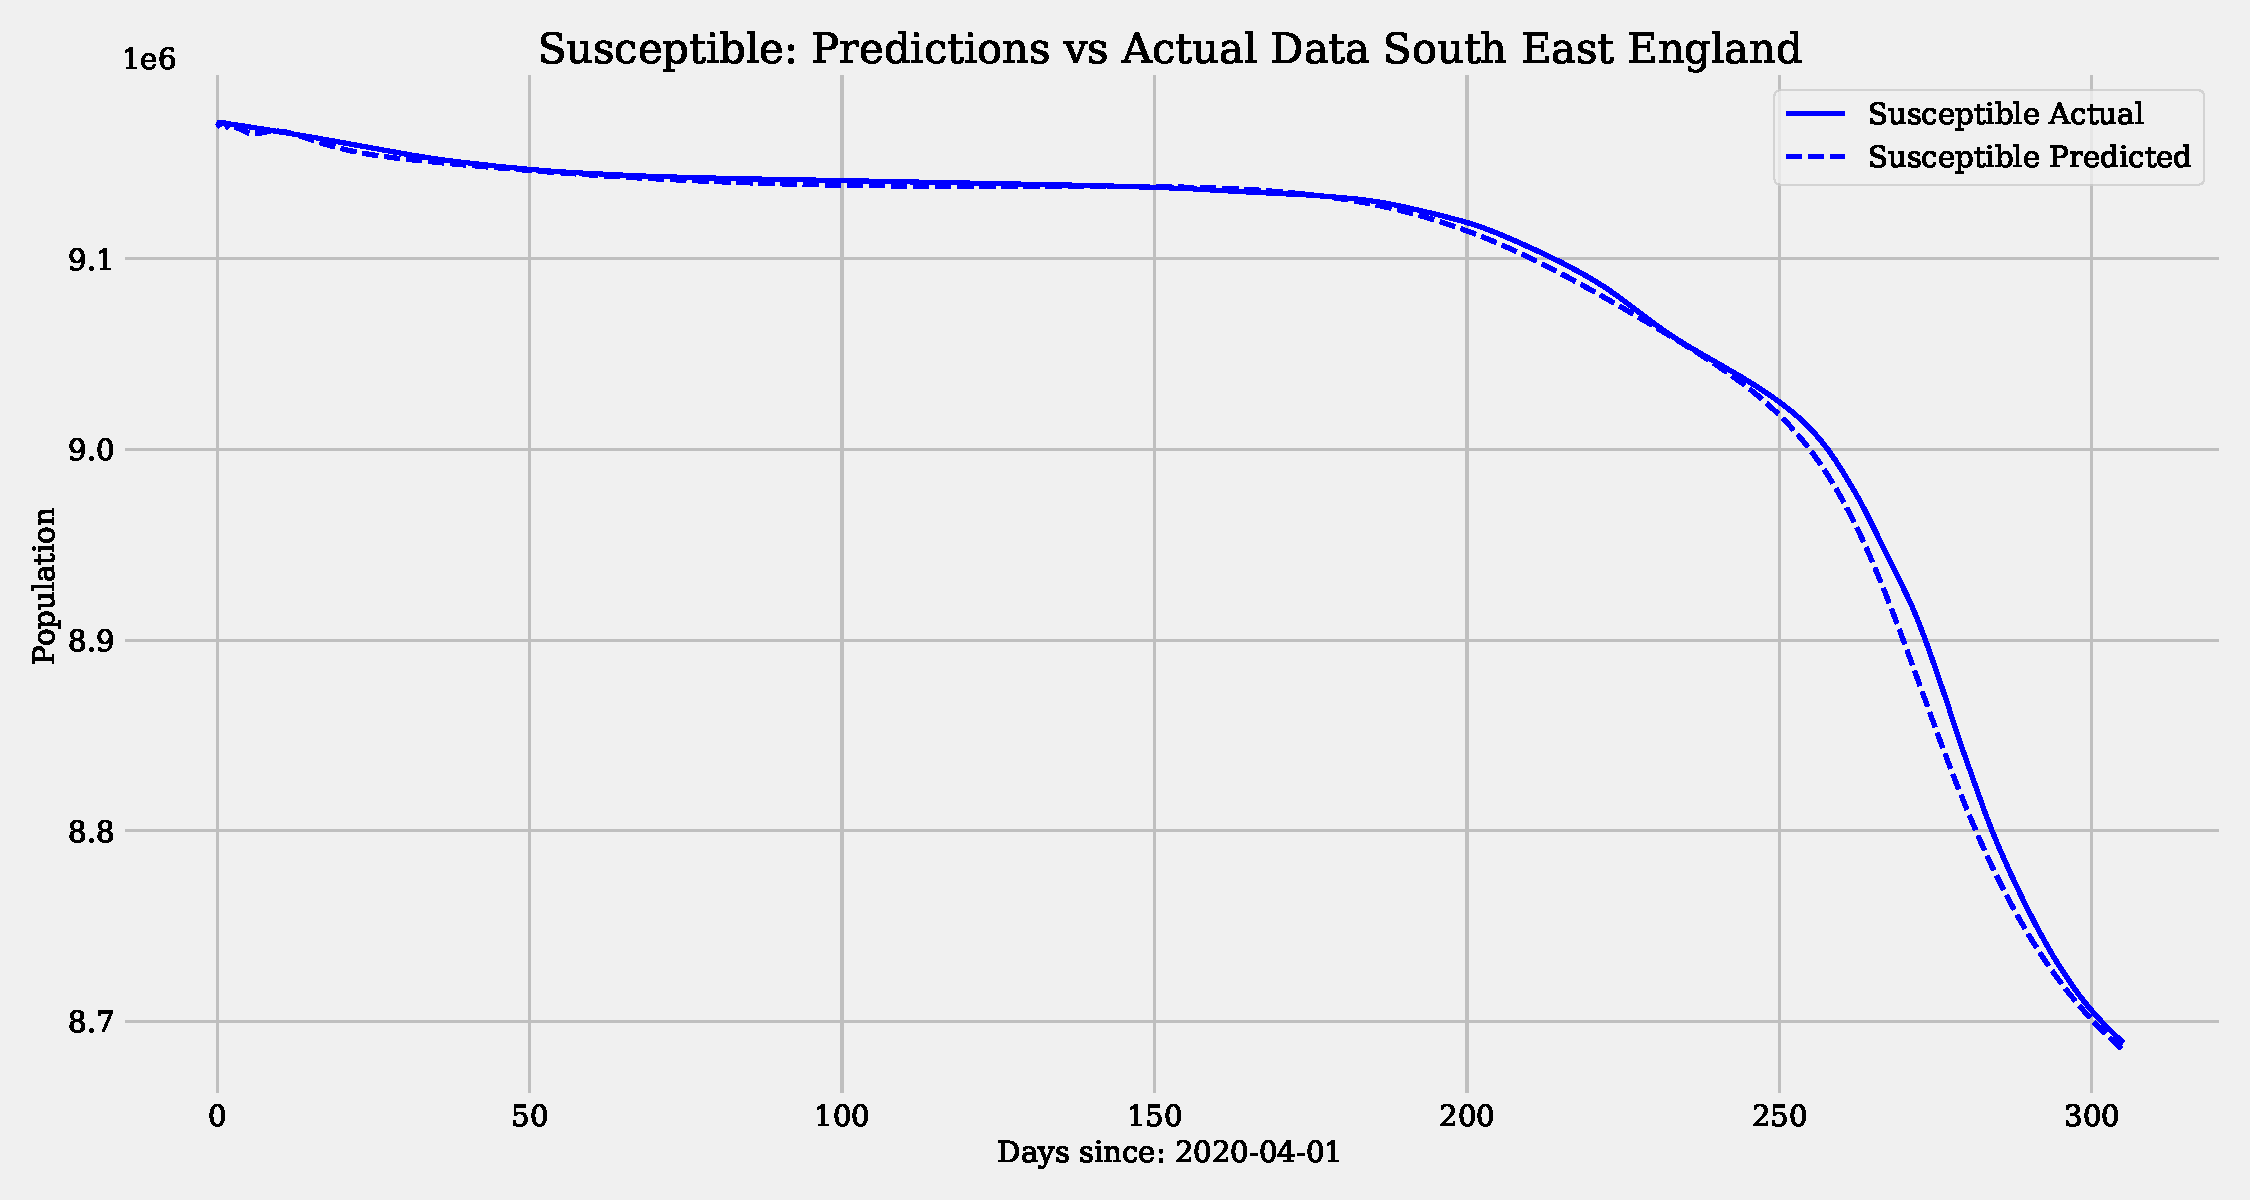
\includegraphics[width=\textwidth]{images/pinn/S_predictions_South East England.pdf}
        \caption{Predicted number of susceptible individuals}
        \label{fig:S_predictions_South East England}
    \end{subfigure}
    \hfill % Ensures that the figures are spaced out evenly
    \begin{subfigure}[t]{0.45\textwidth}
        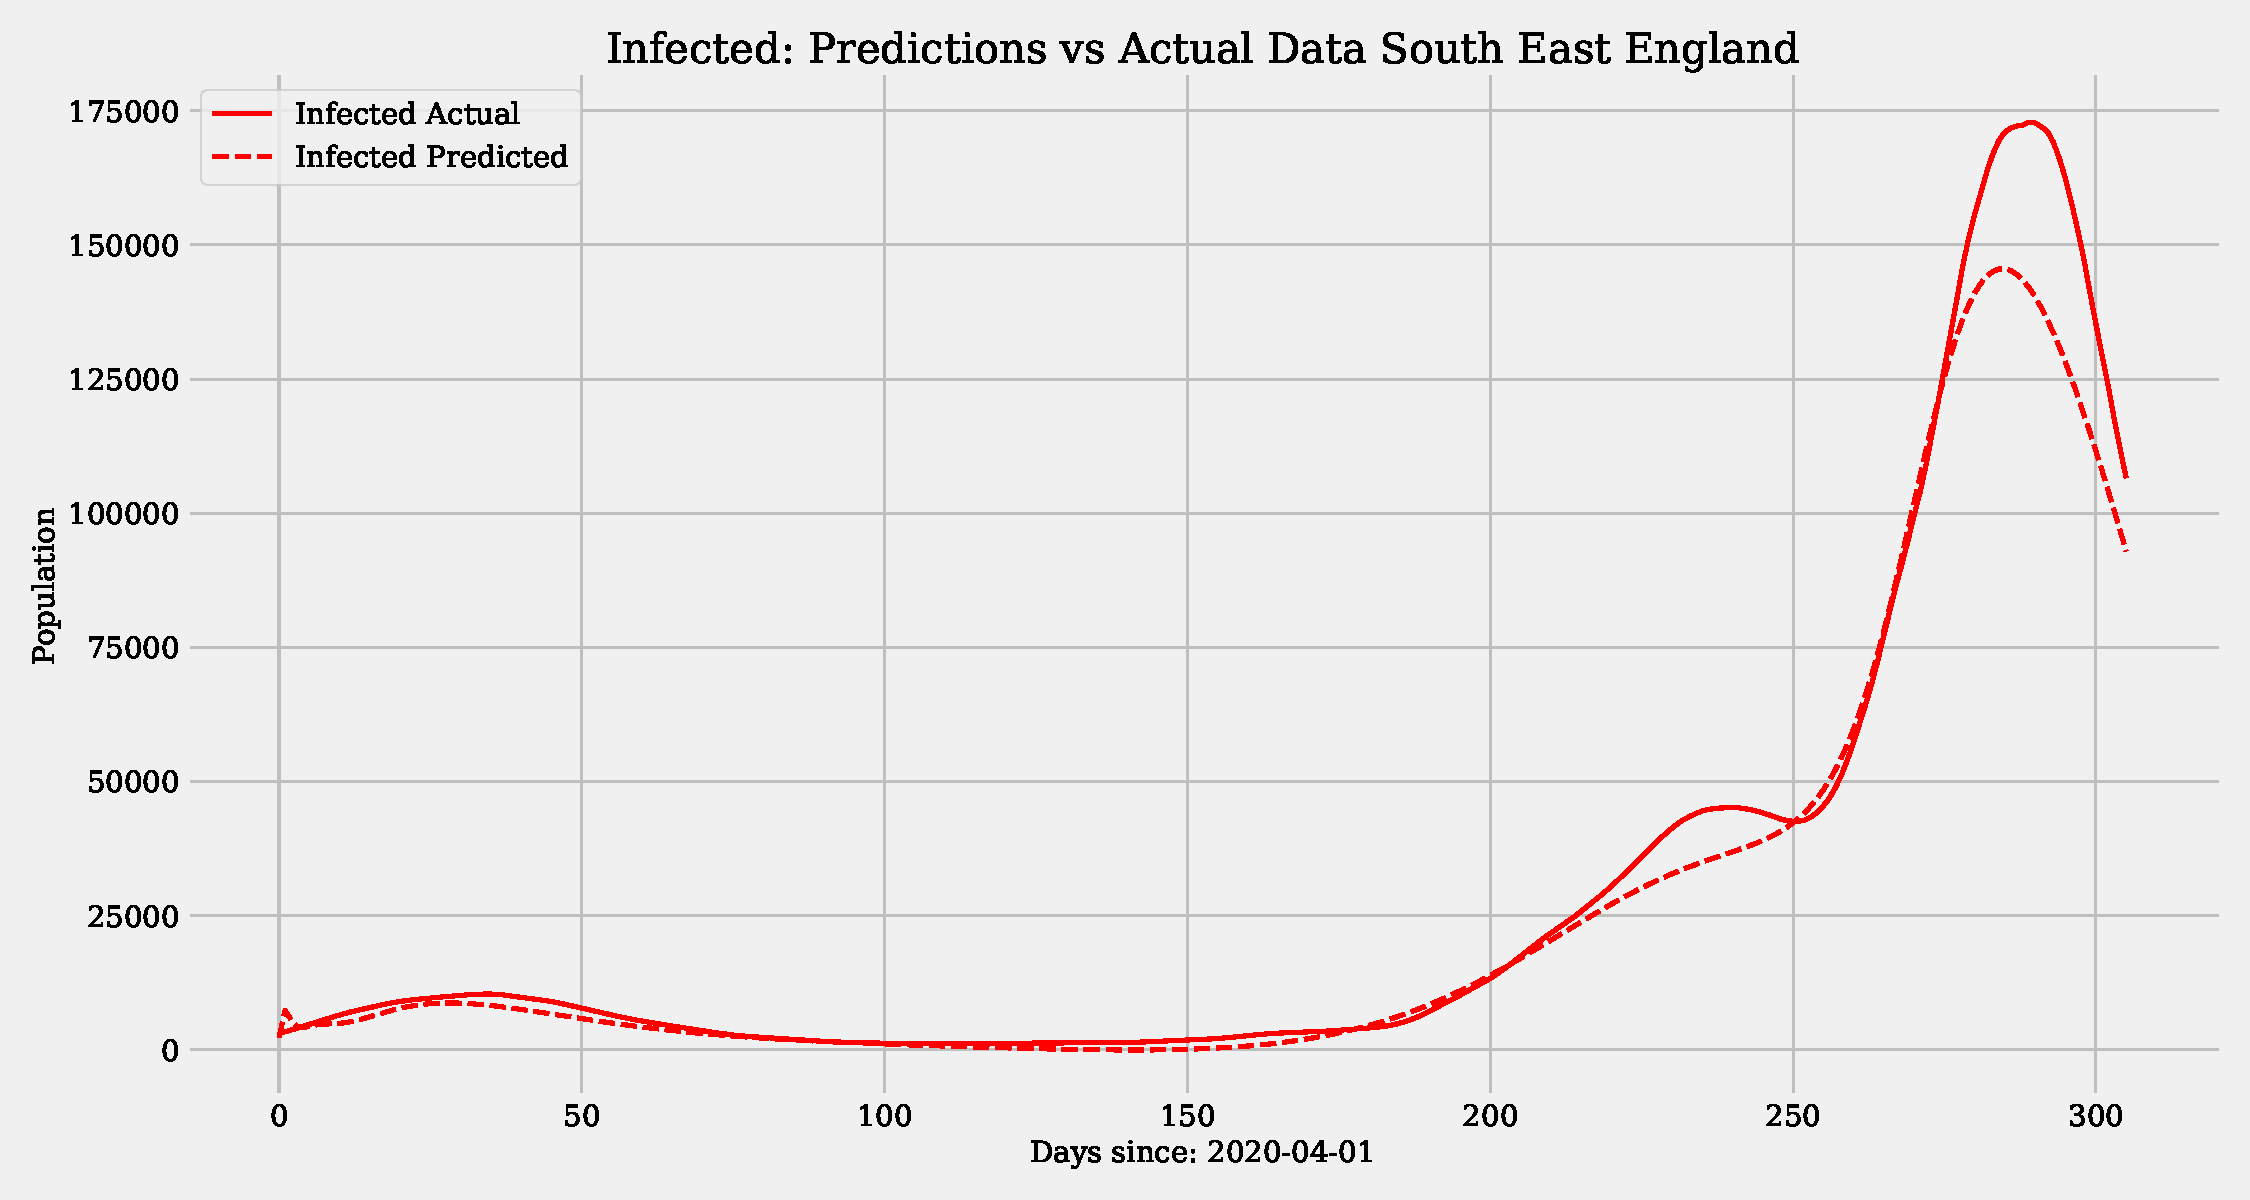
\includegraphics[width=\textwidth]{images/pinn/I_predictions_South East England.pdf}
        \caption{Predicted number of infectious individuals}
        \label{fig:I_predictions_South East England}
    \end{subfigure}

    % Adds a bit of vertical space between the rows of figures
    \vspace{0.5cm}

    \begin{subfigure}[t]{0.45\textwidth}
        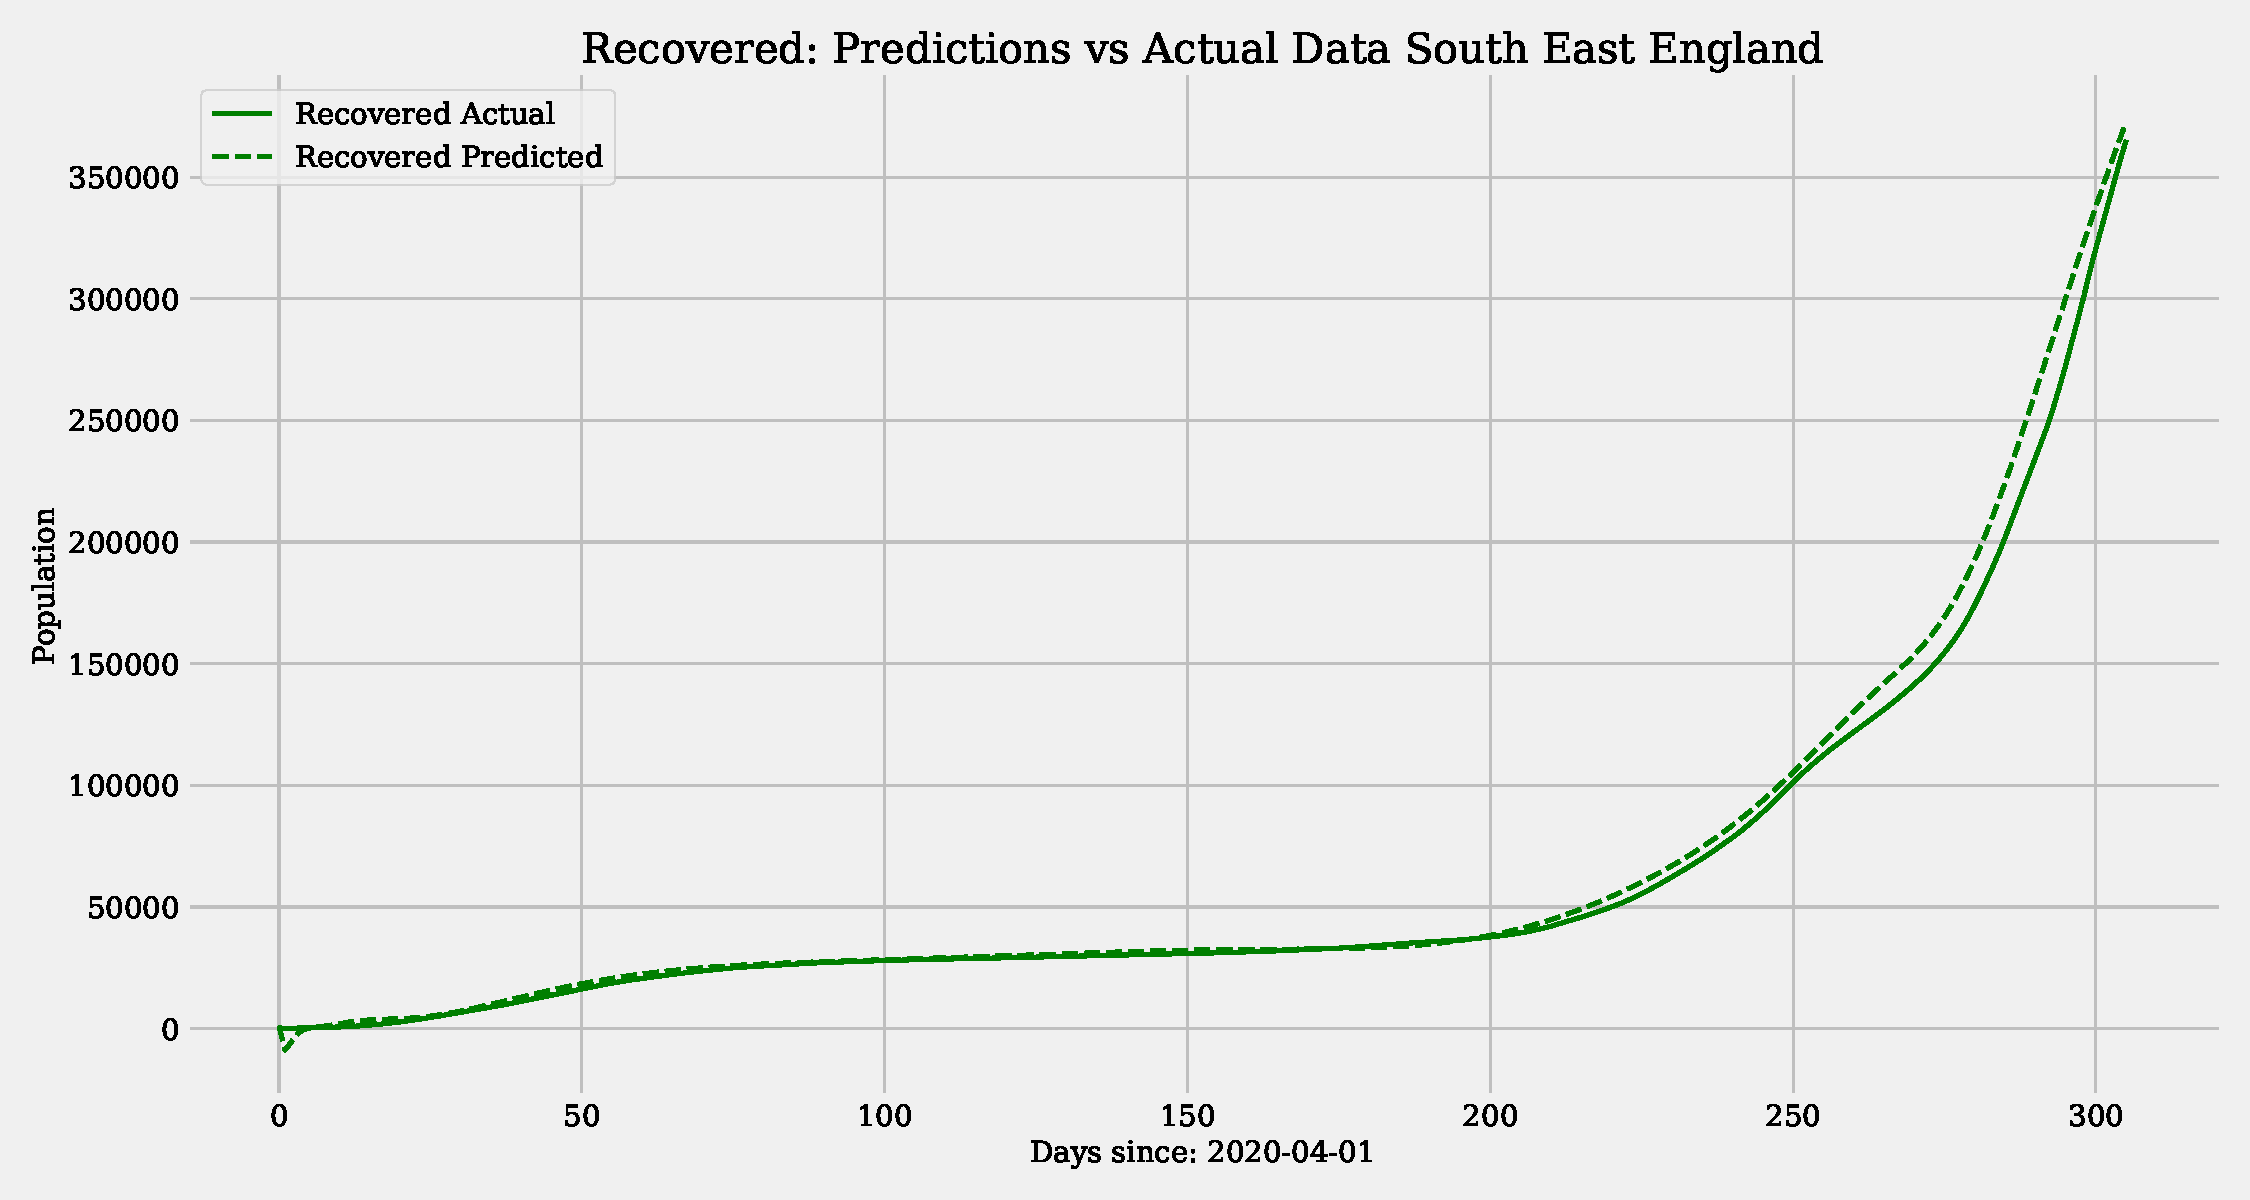
\includegraphics[width=\textwidth]{images/pinn/R_predictions_South East England.pdf}
        \caption{Predicted number of recovered individuals}
        \label{fig:R_predictions_South East England}
    \end{subfigure}
    \hfill % Ensures that the figures are spaced out evenly
    \begin{subfigure}[t]{0.45\textwidth}
        \centering
        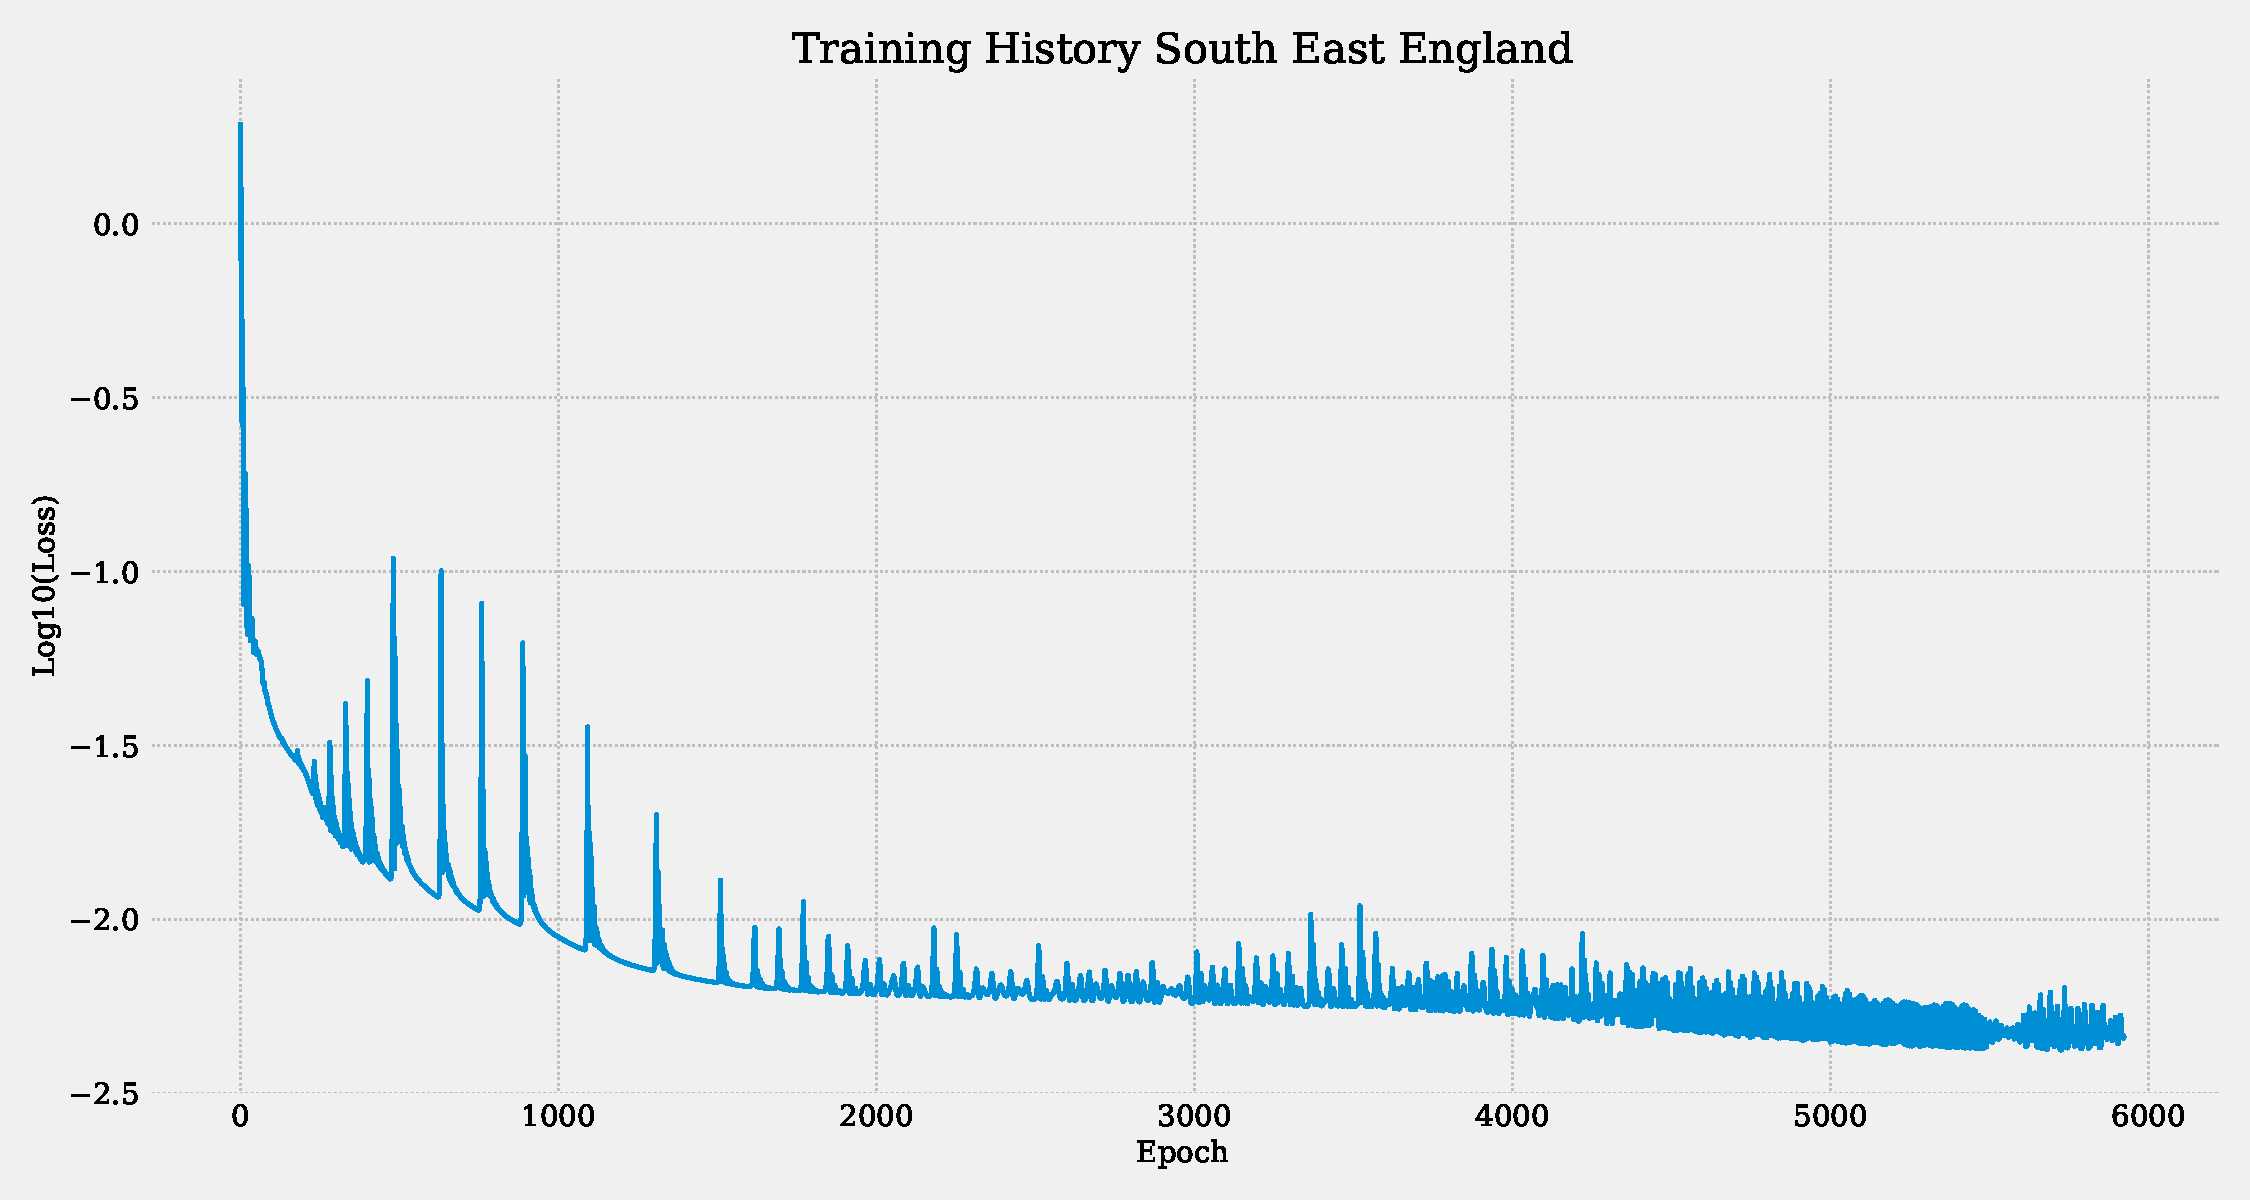
\includegraphics[width=\textwidth]{images/pinn/Training_History_South East England.pdf}
        \caption{Training history of the PINN model}
        \label{fig:Training_History_South East England}
    \end{subfigure}
    \caption{Physics-Informed Neural Network (PINN) model predictions and training history for the South East England region, showcasing the dynamics of susceptible, infectious, and recovered populations alongside model training progression.}
    \label{fig:PINN_South East England_Comprehensive}

\end{figure*}

\begin{figure}
    \centering
    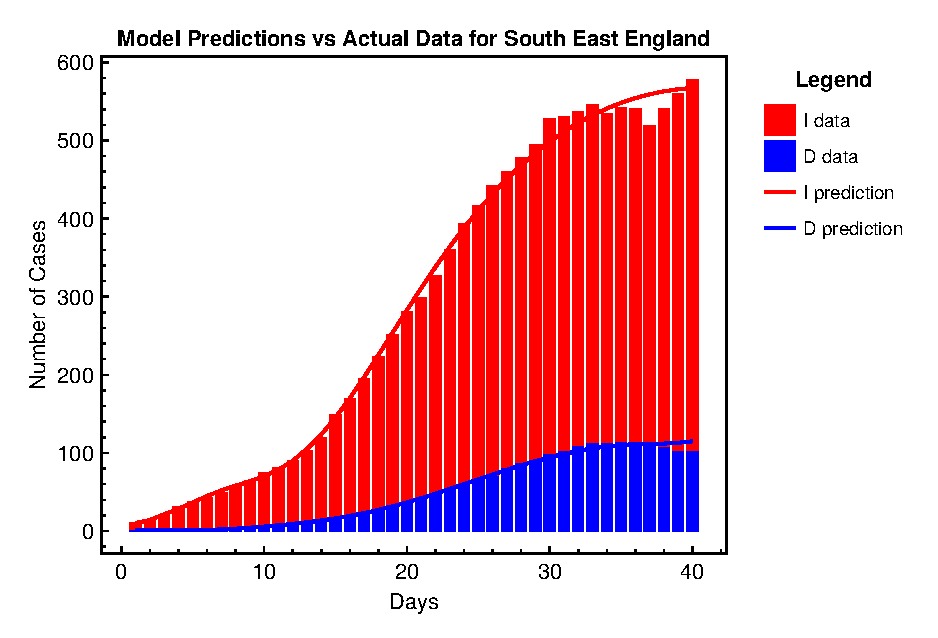
\includegraphics[width=0.8\textwidth]{images/ude/South East England_infected_death_data.pdf}
    \caption{Predicted number of infected and deceased individuals}
    \label{fig:ude_South East England}
\end{figure}

\begin{figure*}
    \centering
    \begin{subfigure}[t]{0.45\textwidth}
        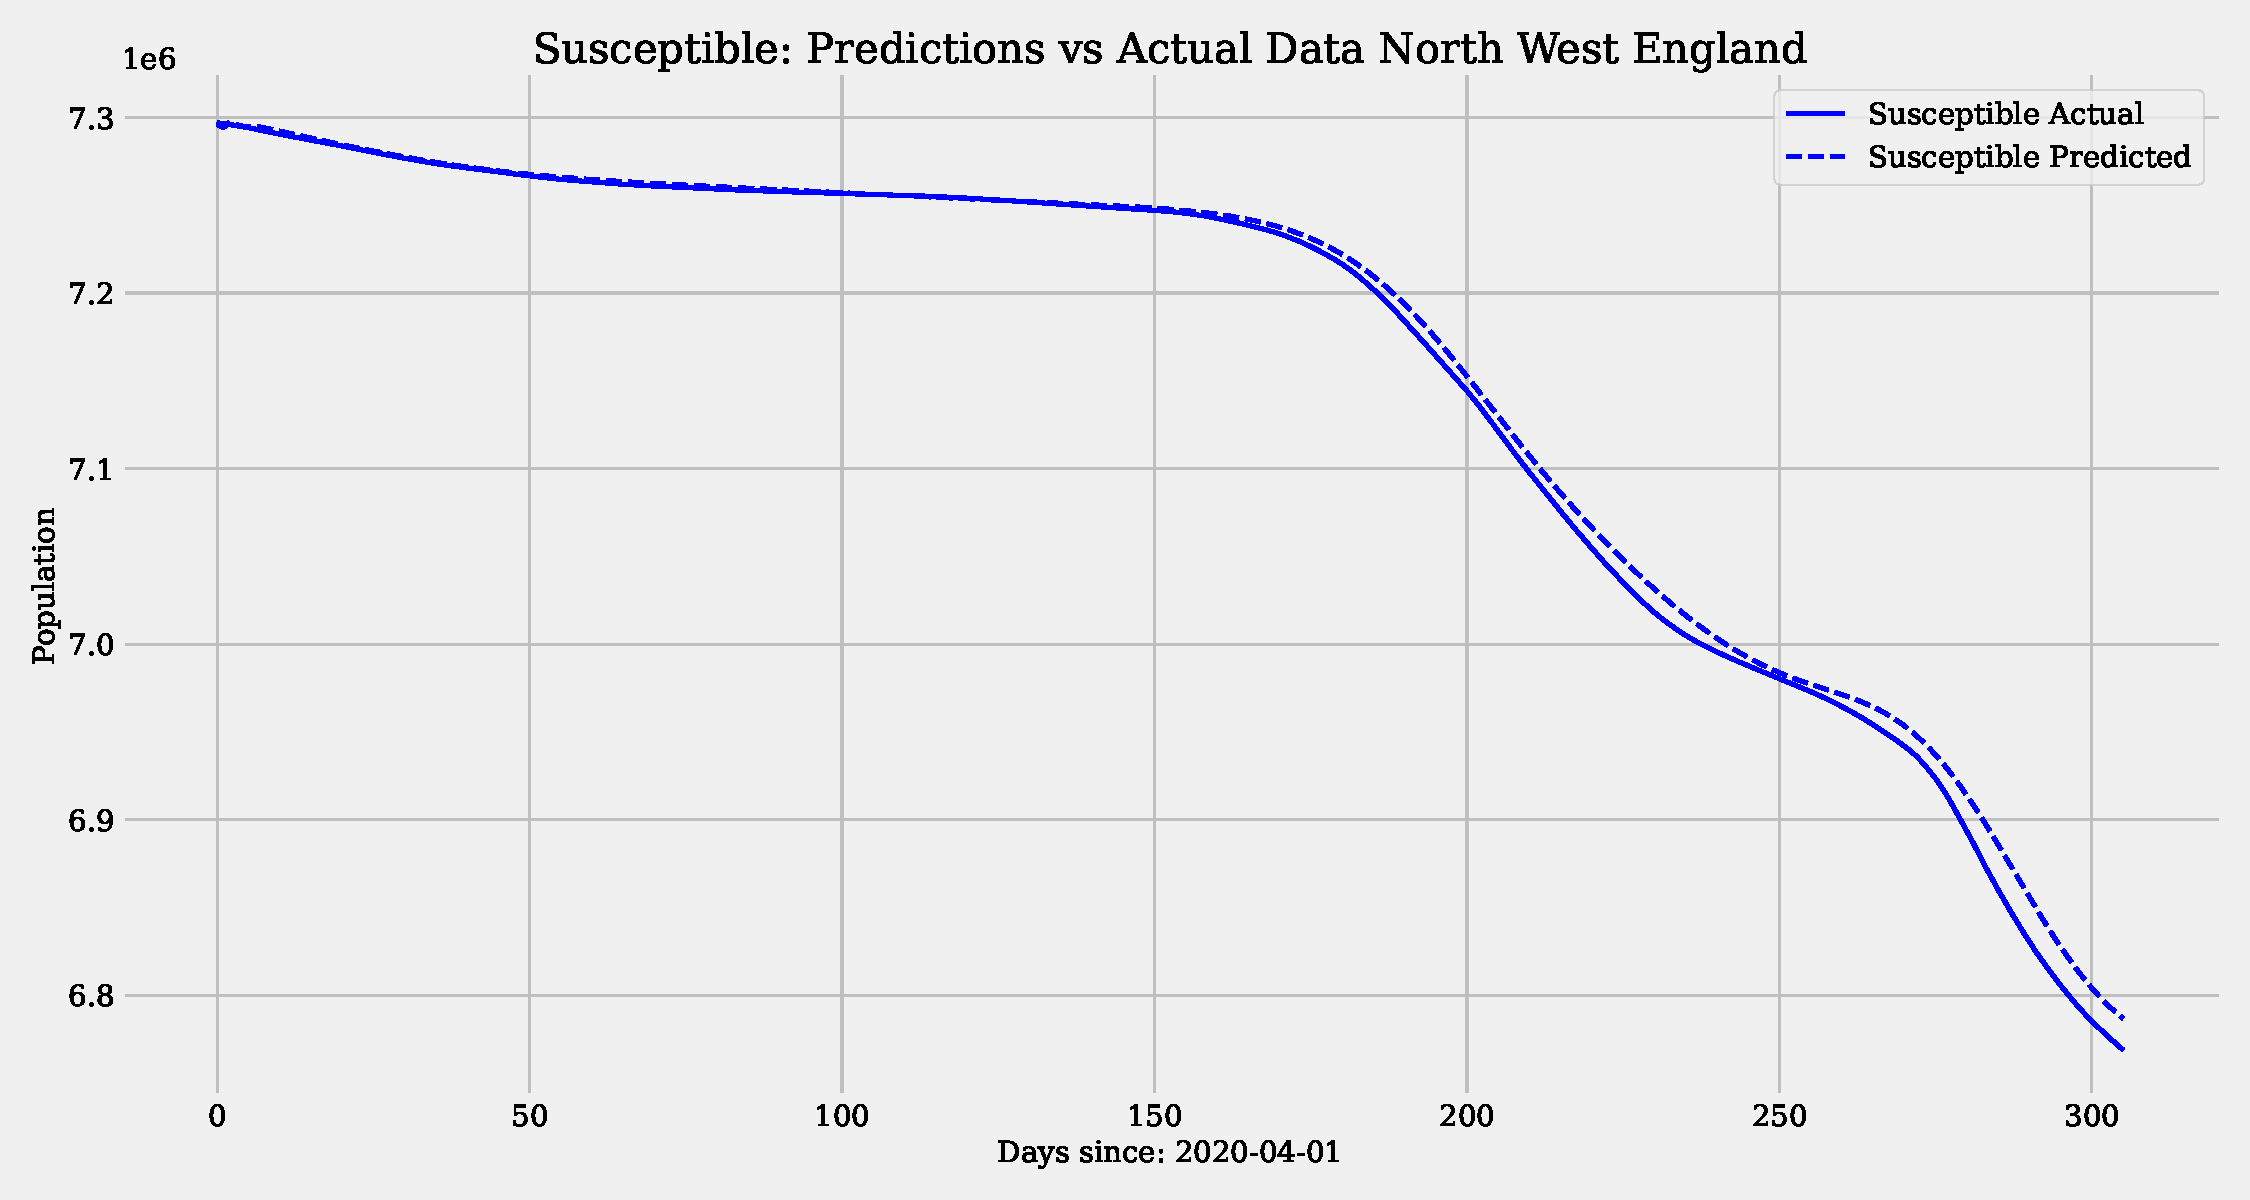
\includegraphics[width=\textwidth]{images/pinn/S_predictions_North West England.pdf}
        \caption{Predicted number of susceptible individuals}
        \label{fig:S_predictions_North West England}
    \end{subfigure}
    \hfill % Ensures that the figures are spaced out evenly
    \begin{subfigure}[t]{0.45\textwidth}
        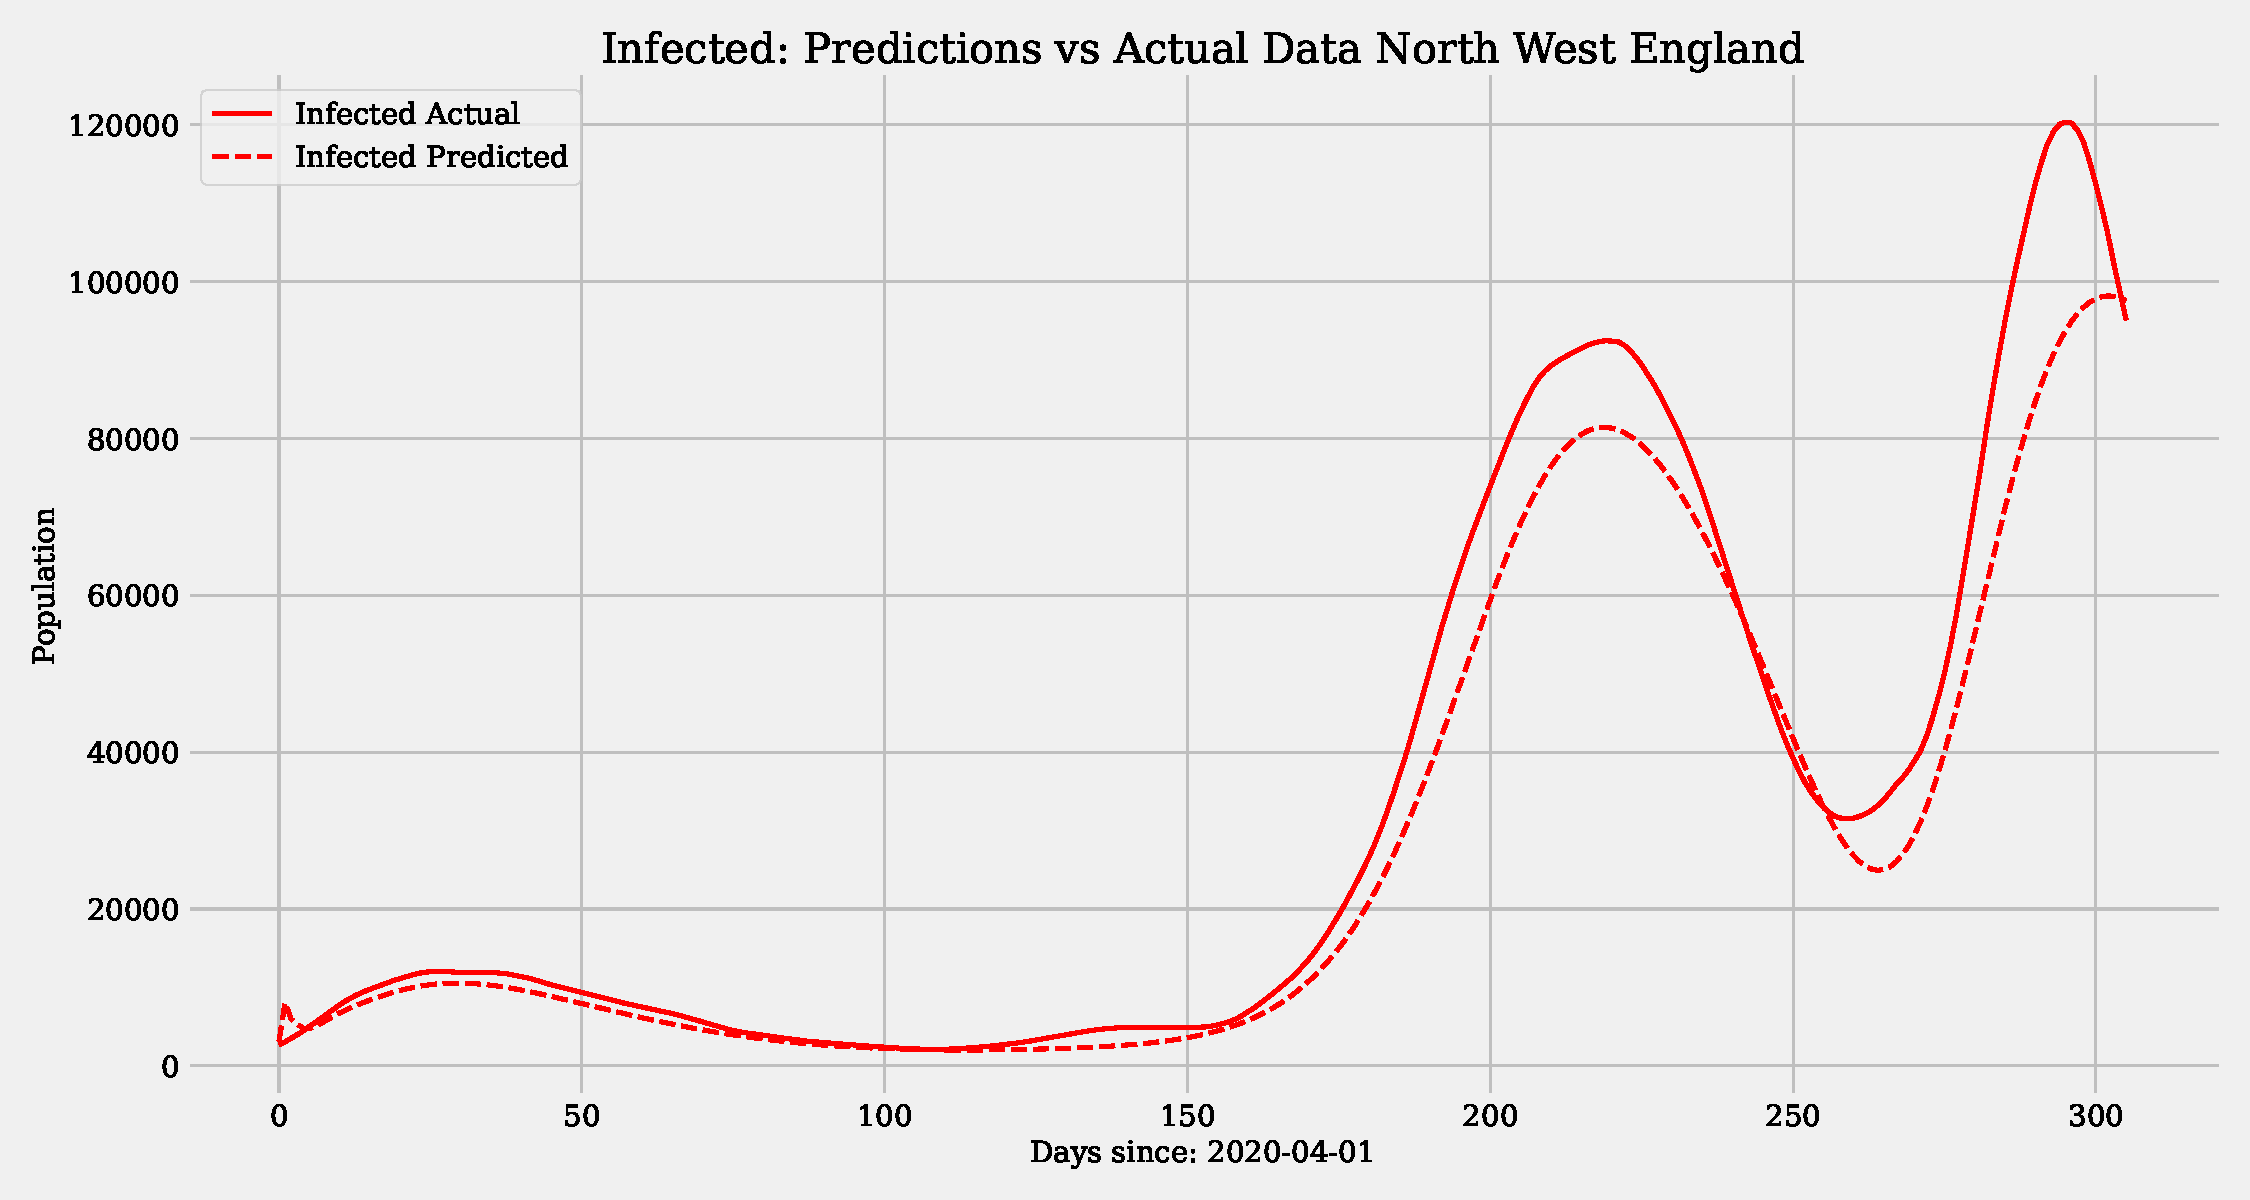
\includegraphics[width=\textwidth]{images/pinn/I_predictions_North West England.pdf}
        \caption{Predicted number of infectious individuals}
        \label{fig:I_predictions_North West England}
    \end{subfigure}

    % Adds a bit of vertical space between the rows of figures
    \vspace{0.5cm}

    \begin{subfigure}[t]{0.45\textwidth}
        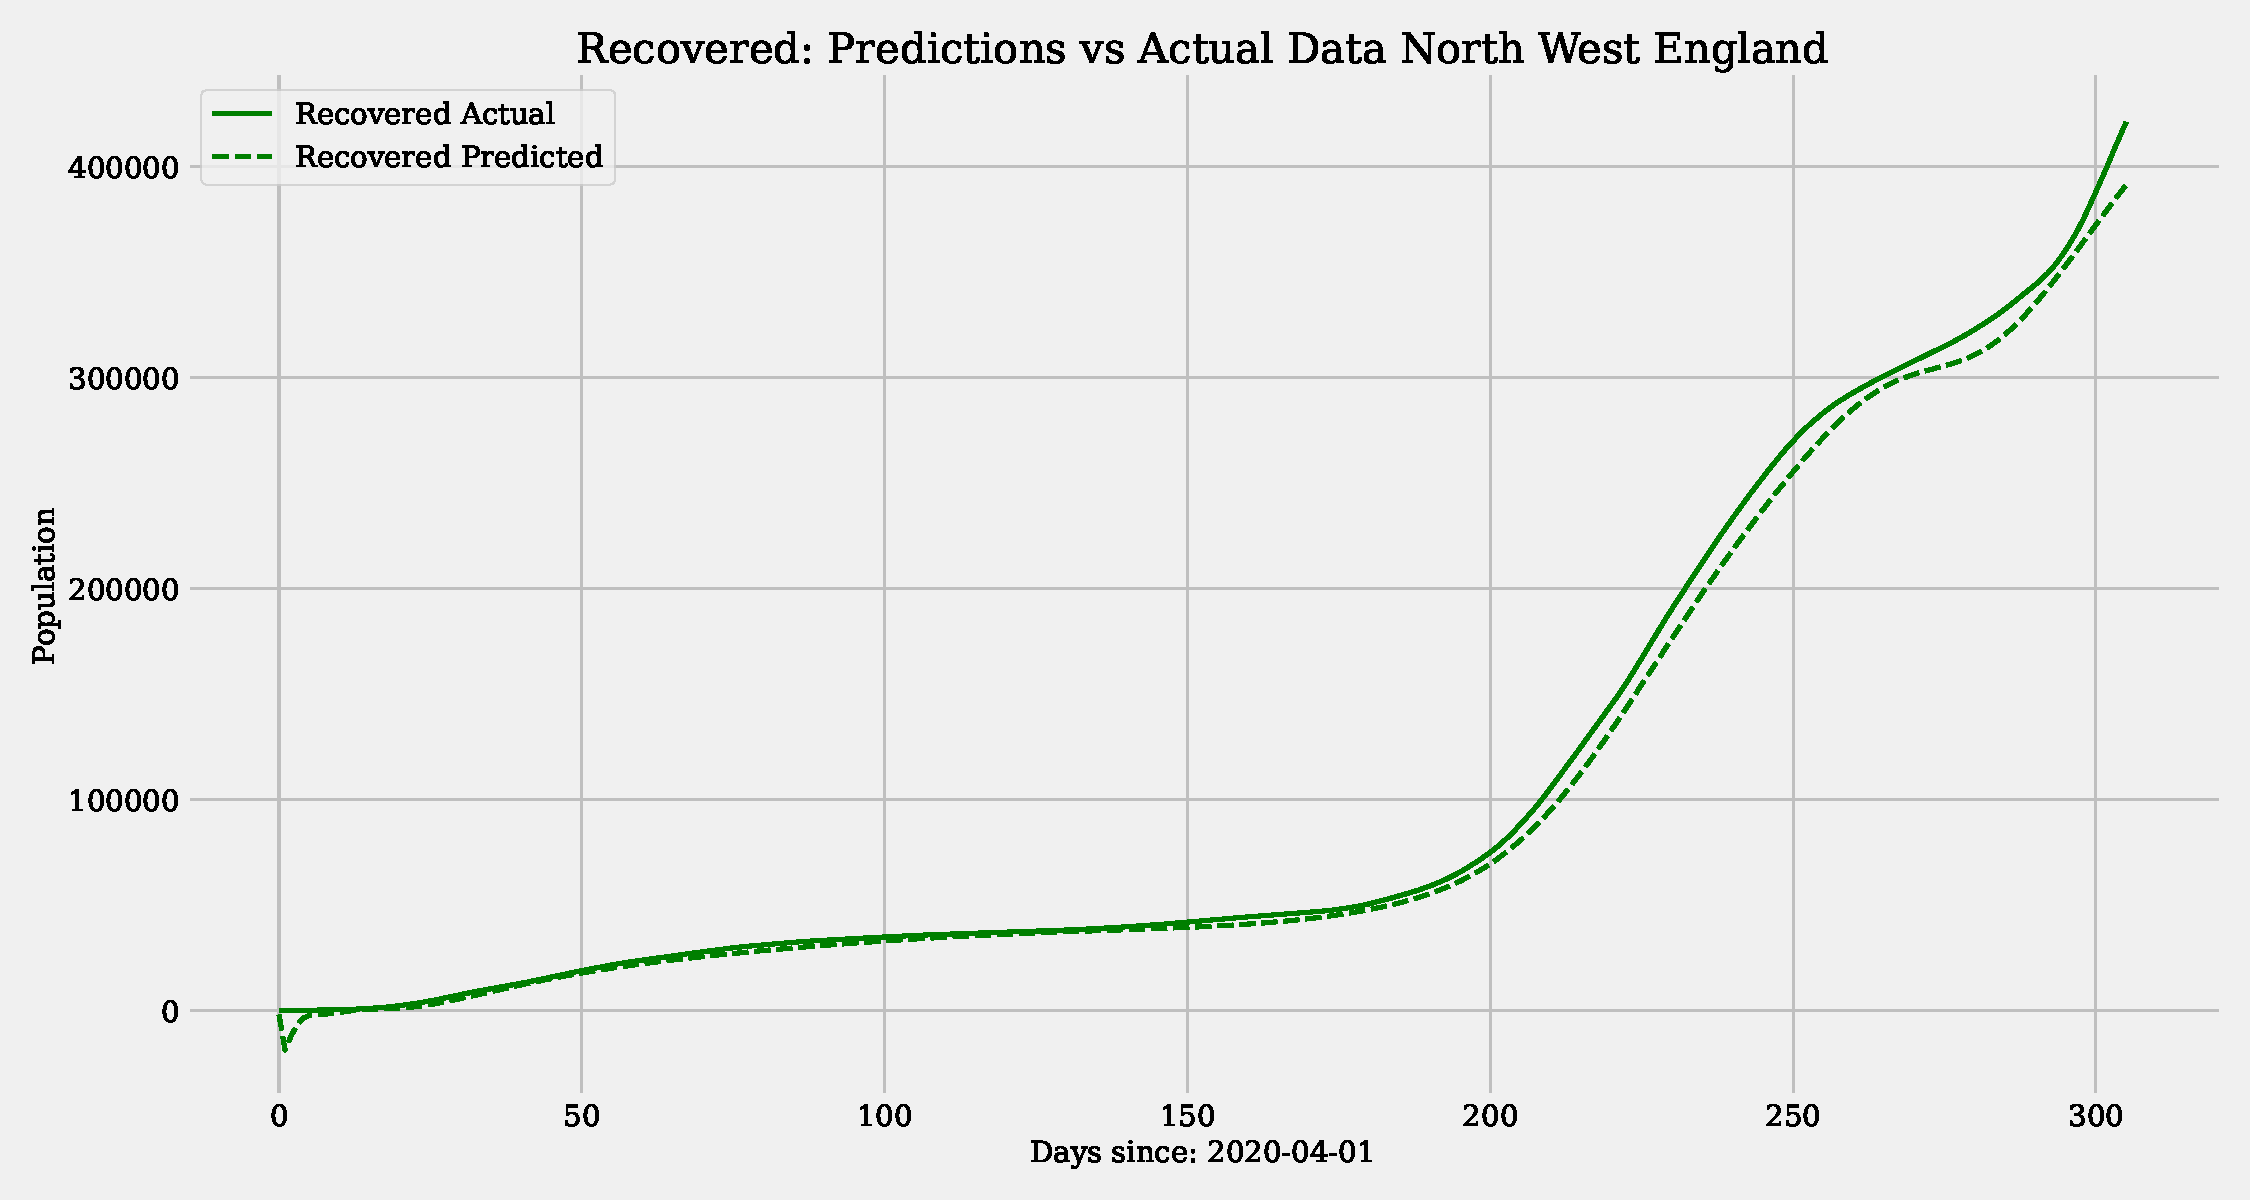
\includegraphics[width=\textwidth]{images/pinn/R_predictions_North West England.pdf}
        \caption{Predicted number of recovered individuals}
        \label{fig:R_predictions_North West England}
    \end{subfigure}
    \hfill % Ensures that the figures are spaced out evenly
    \begin{subfigure}[t]{0.45\textwidth}
        \centering
        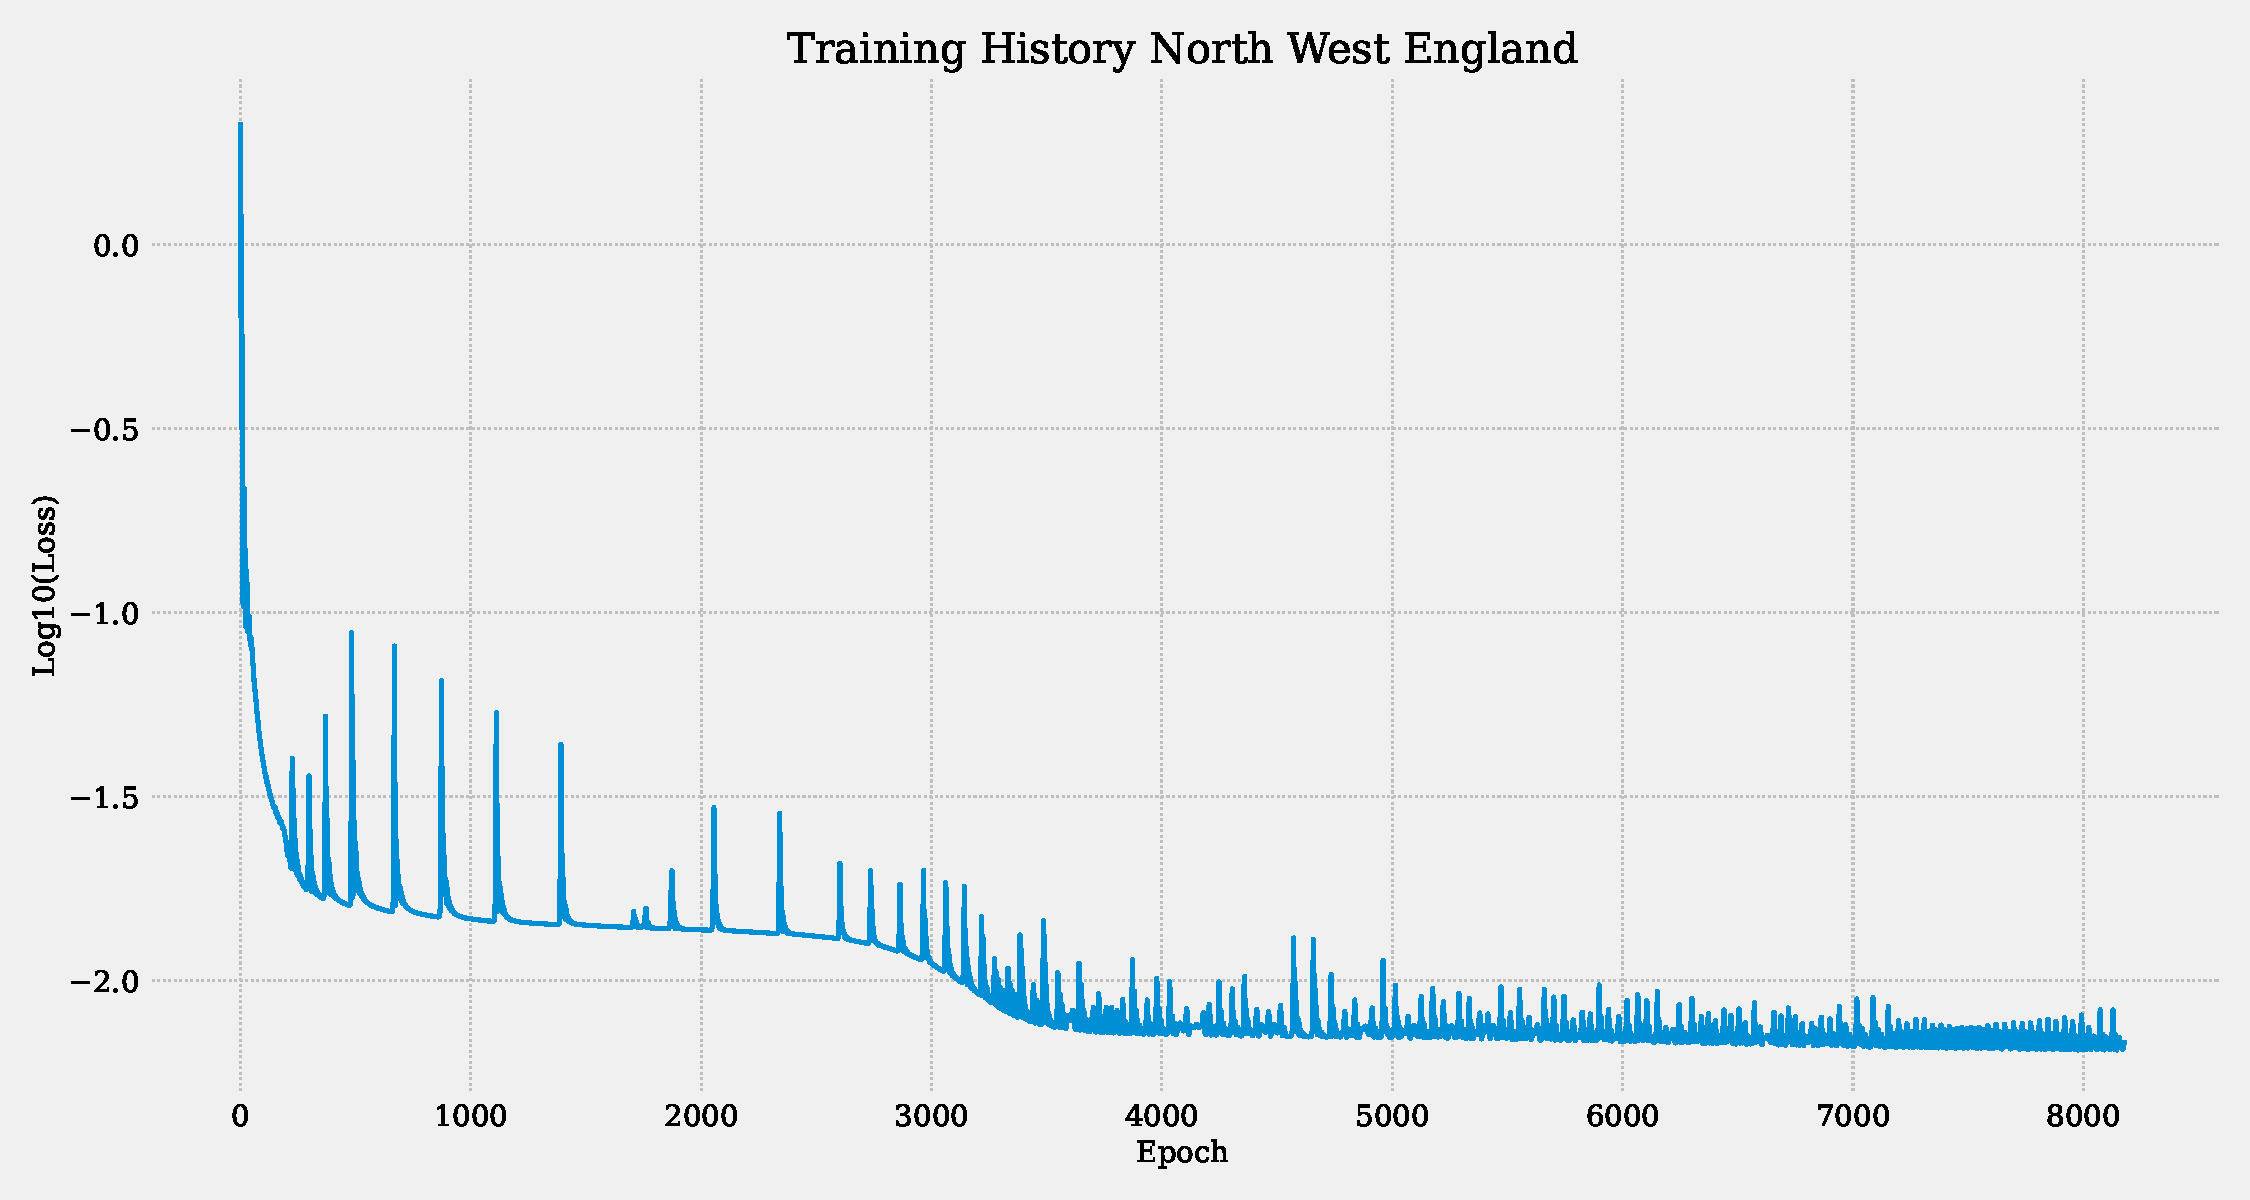
\includegraphics[width=\textwidth]{images/pinn/Training_History_North West England.pdf}
        \caption{Training history of the PINN model}
        \label{fig:Training_History_North West England}
    \end{subfigure}
    \caption{Physics-Informed Neural Network (PINN) model predictions and training history for the North West England region, showcasing the dynamics of susceptible, infectious, and recovered populations alongside model training progression.}
    \label{fig:PINN_North West England_Comprehensive}
\end{figure*}

\begin{figure}
    \centering
    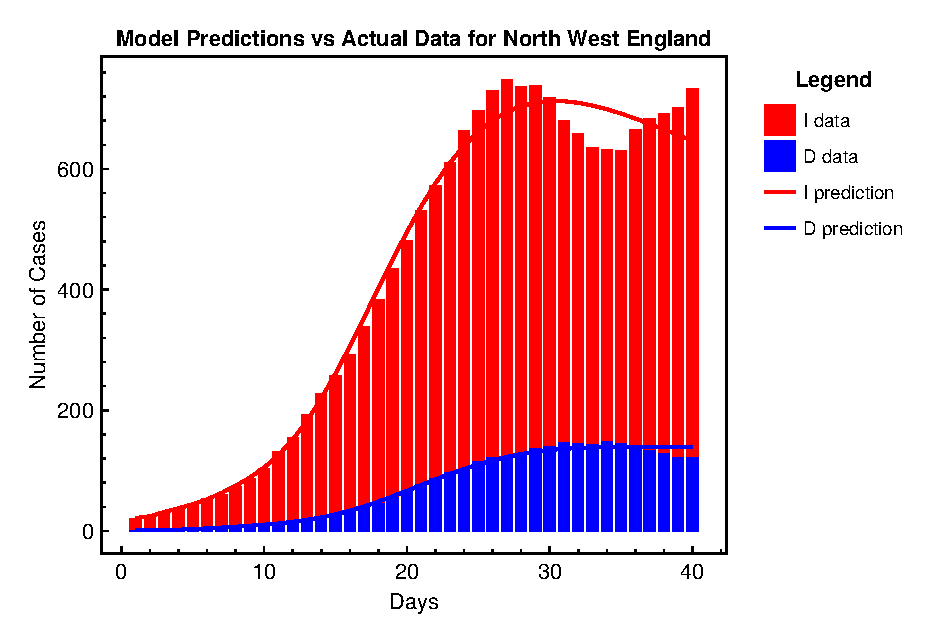
\includegraphics[width=0.8\textwidth]{images/ude/North West England_infected_death_data.pdf}
    \caption{Predicted number of infected and deceased individuals}
    \label{fig:ude_North West England}
\end{figure}


\begin{figure*}
    \centering
    \begin{subfigure}[t]{0.45\textwidth}
        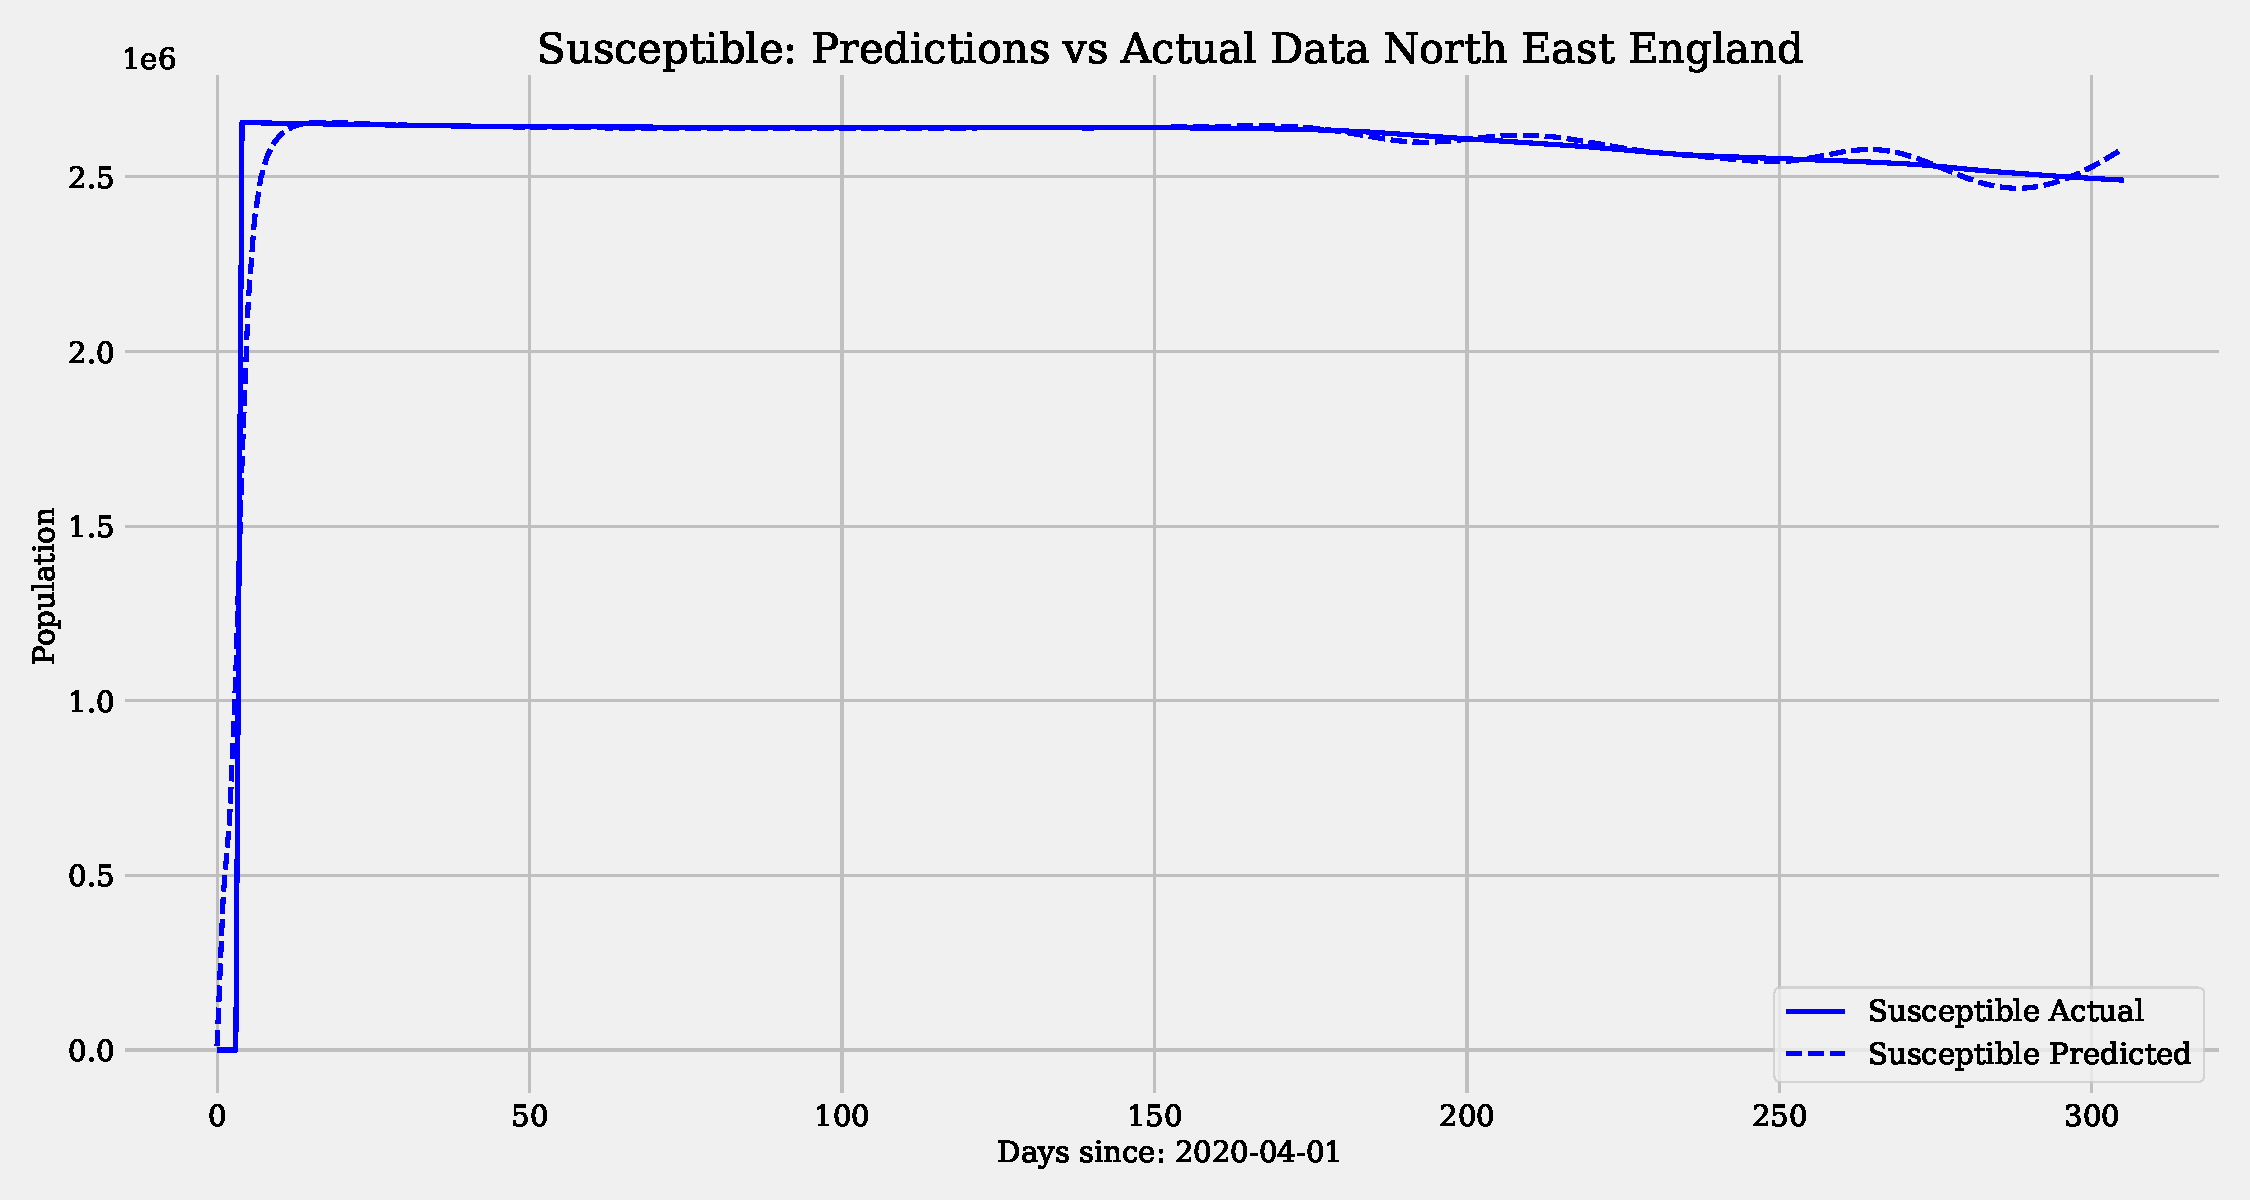
\includegraphics[width=\textwidth]{images/pinn/S_predictions_North East England.pdf}
        \caption{Predicted number of susceptible individuals}
        \label{fig:S_predictions_North East England}
    \end{subfigure}
    \hfill % Ensures that the figures are spaced out evenly
    \begin{subfigure}[t]{0.45\textwidth}
        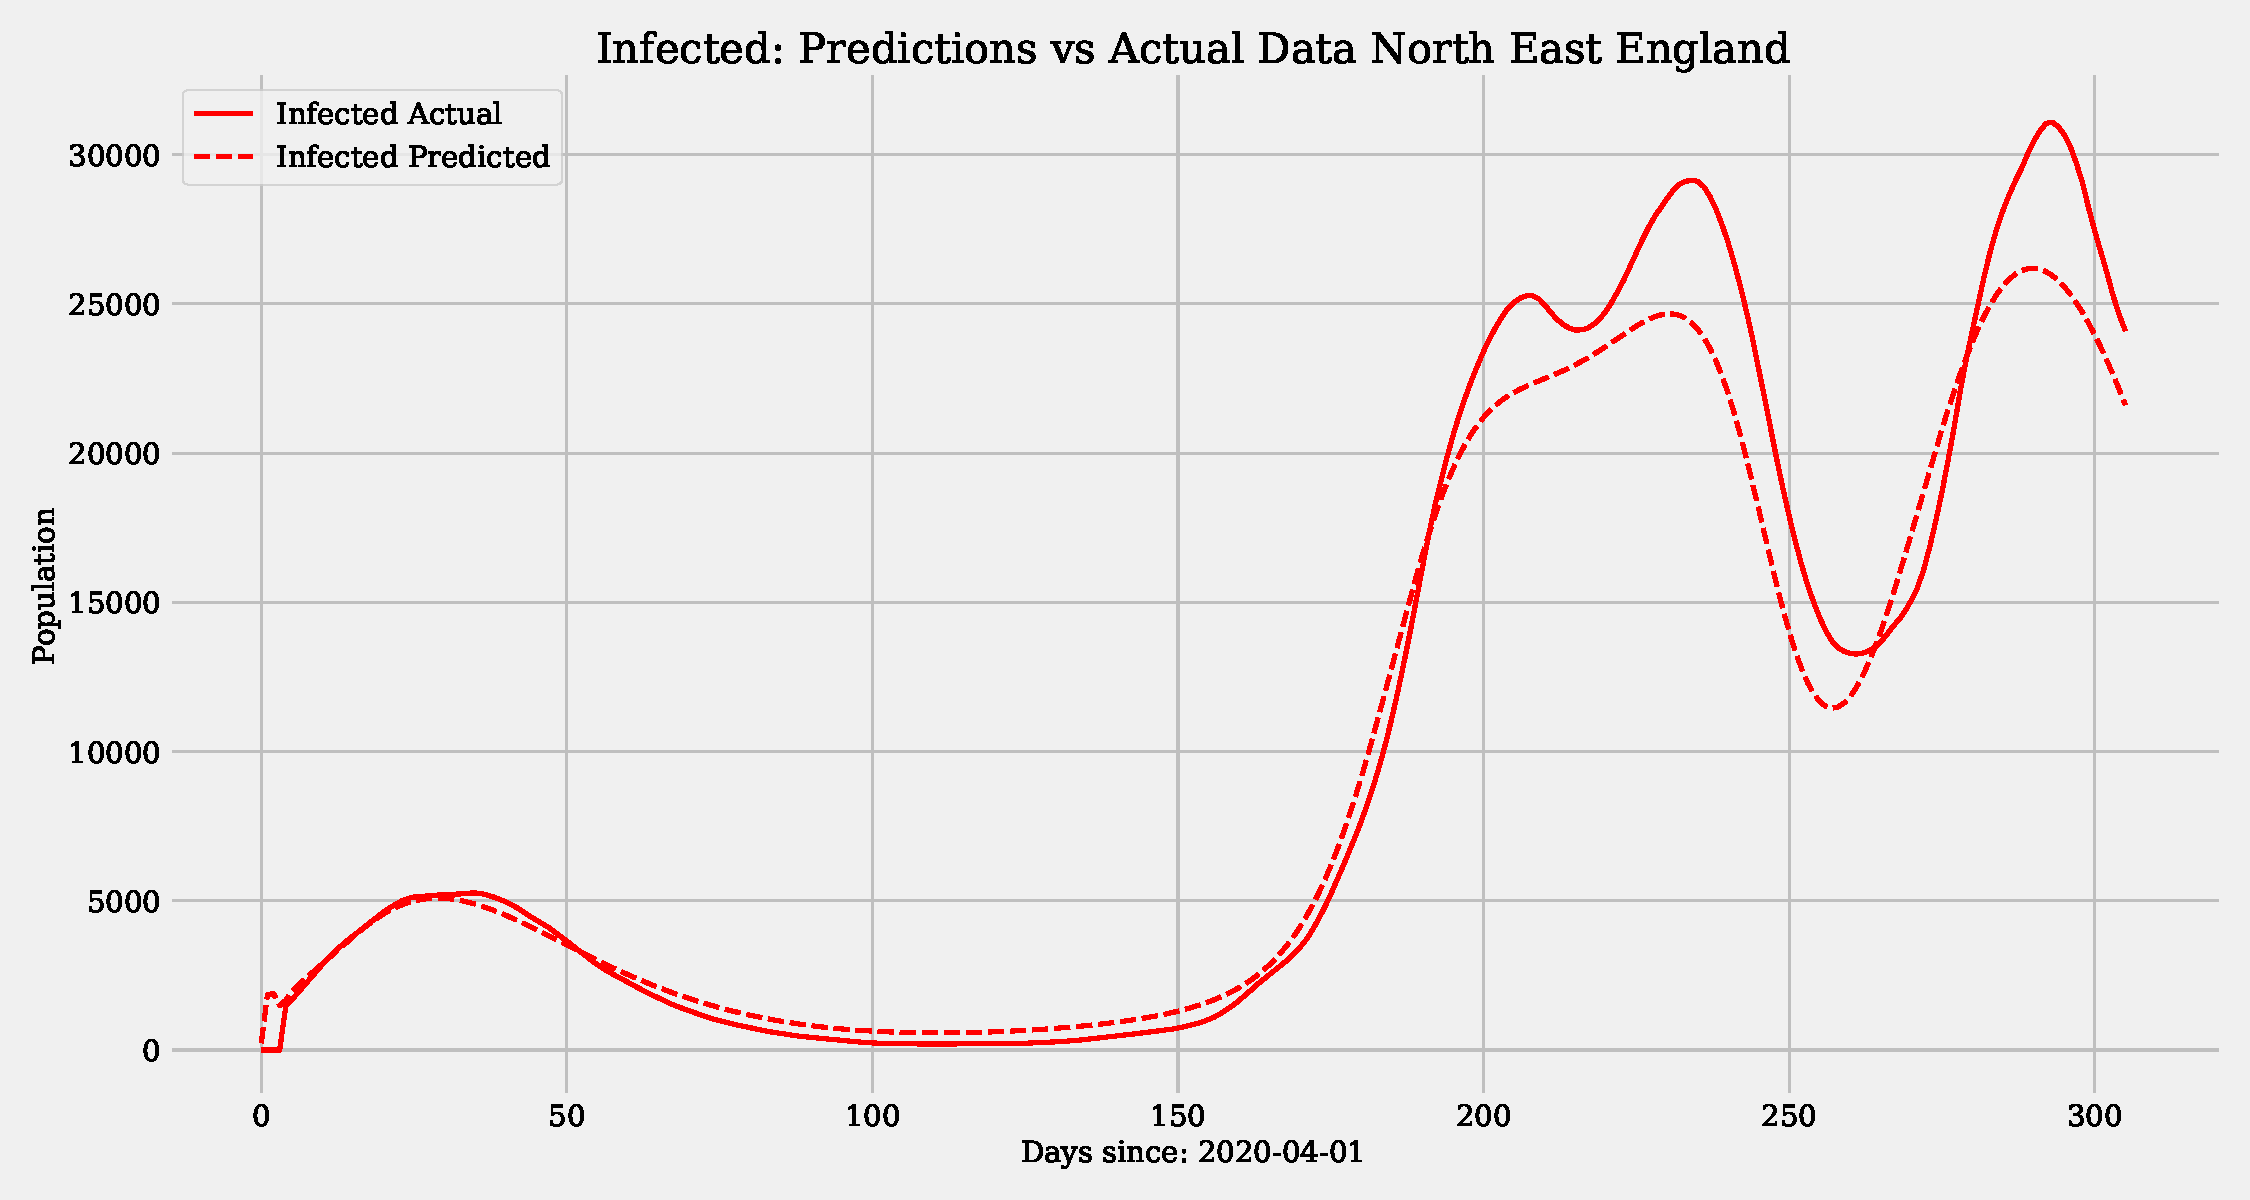
\includegraphics[width=\textwidth]{images/pinn/I_predictions_North East England.pdf}
        \caption{Predicted number of infectious individuals}
        \label{fig:I_predictions_North East England}
    \end{subfigure}

    % Adds a bit of vertical space between the rows of figures
    \vspace{0.5cm}

    \begin{subfigure}[t]{0.45\textwidth}
        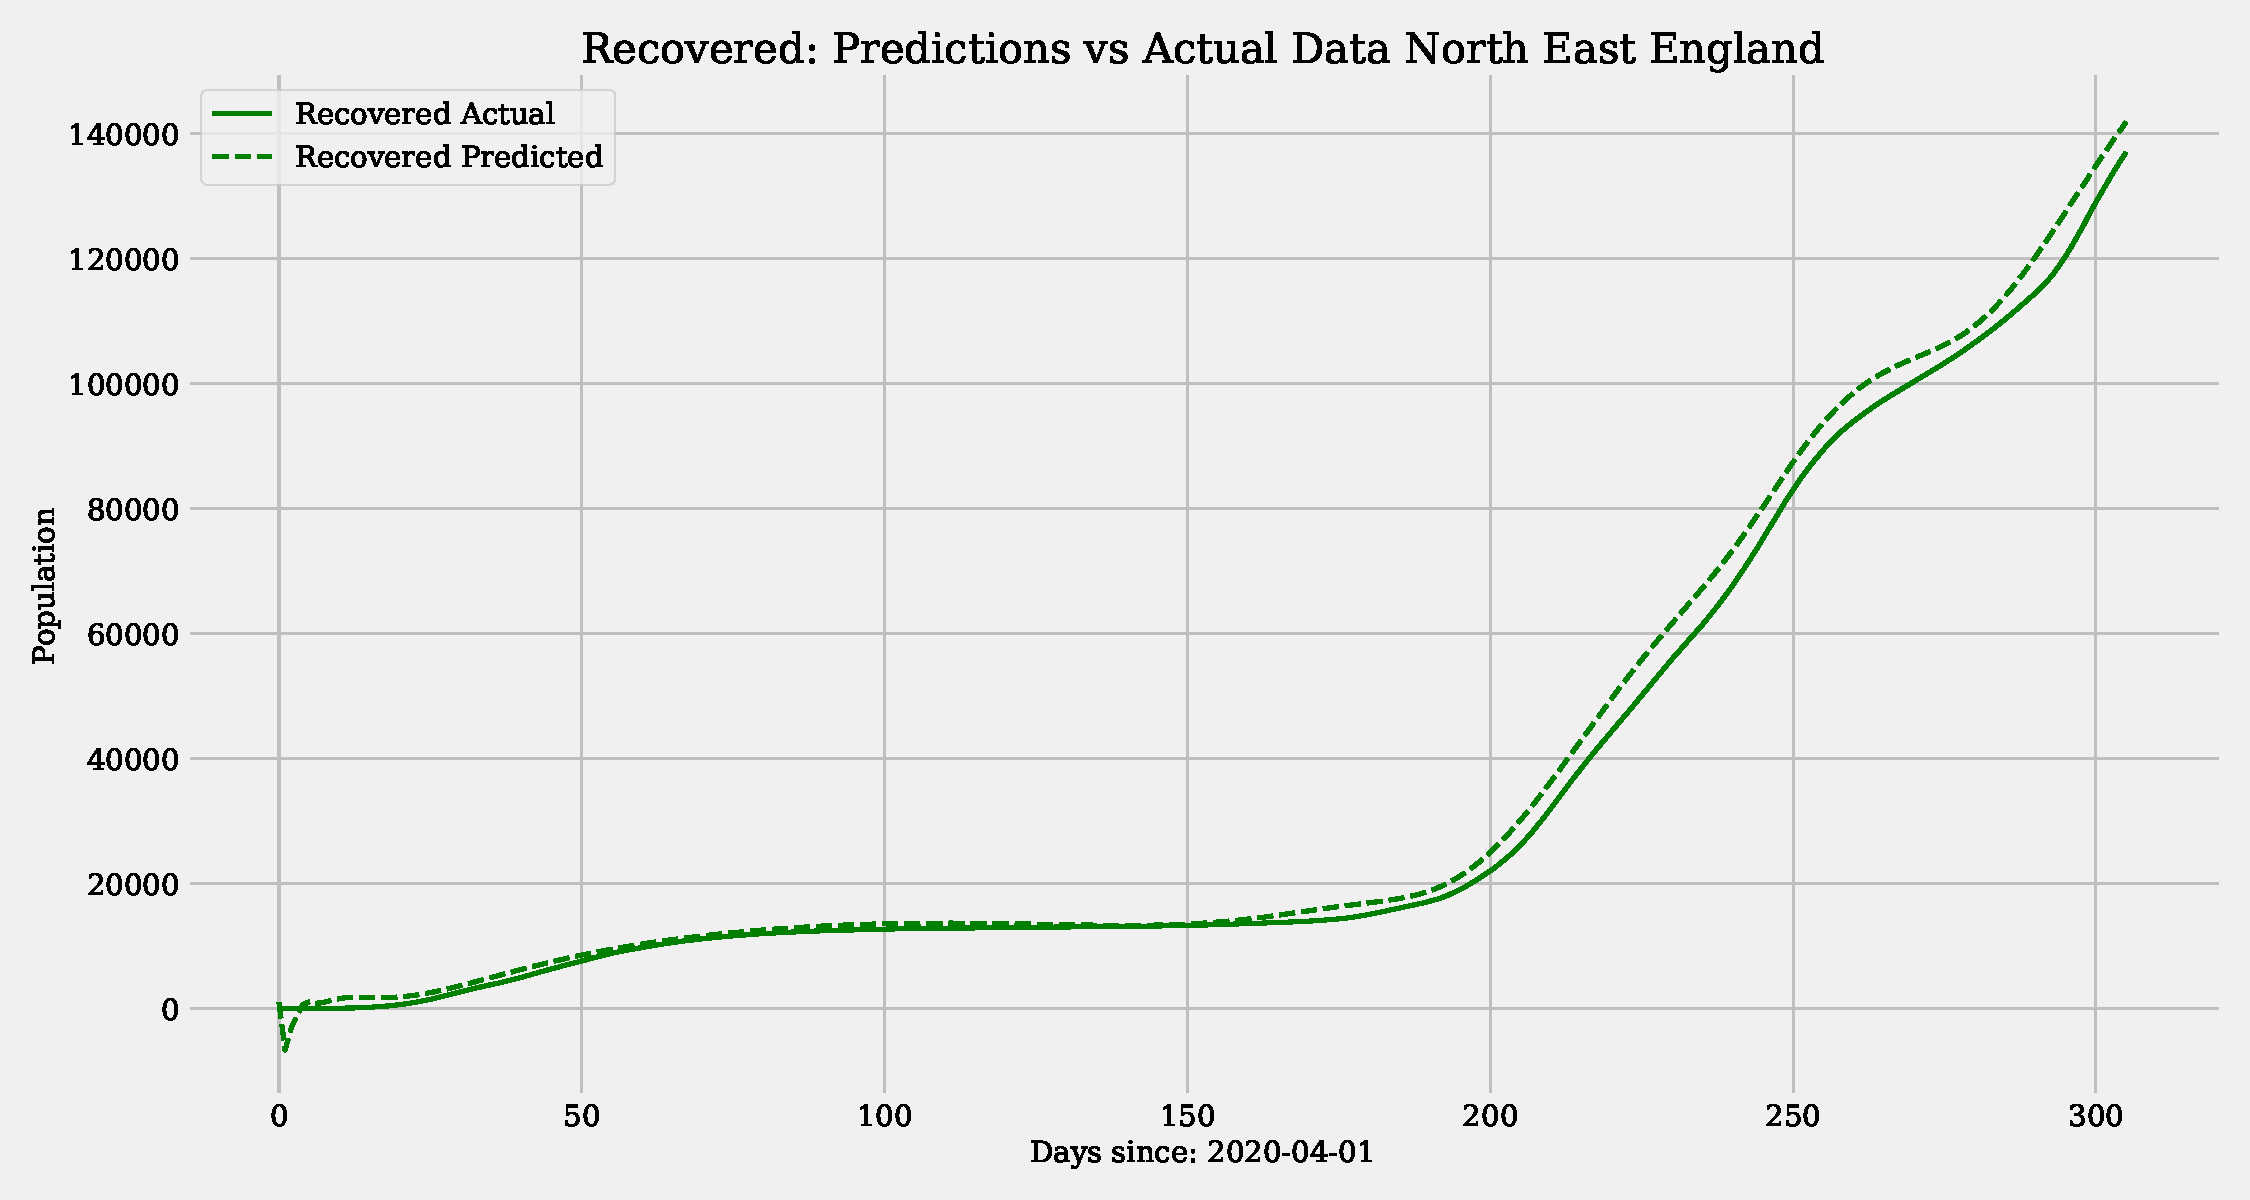
\includegraphics[width=\textwidth]{images/pinn/R_predictions_North East England.pdf}
        \caption{Predicted number of recovered individuals}
        \label{fig:R_predictions_North East England}
    \end{subfigure}
    \hfill % Ensures that the figures are spaced out evenly
    \begin{subfigure}[t]{0.45\textwidth}
        \centering
        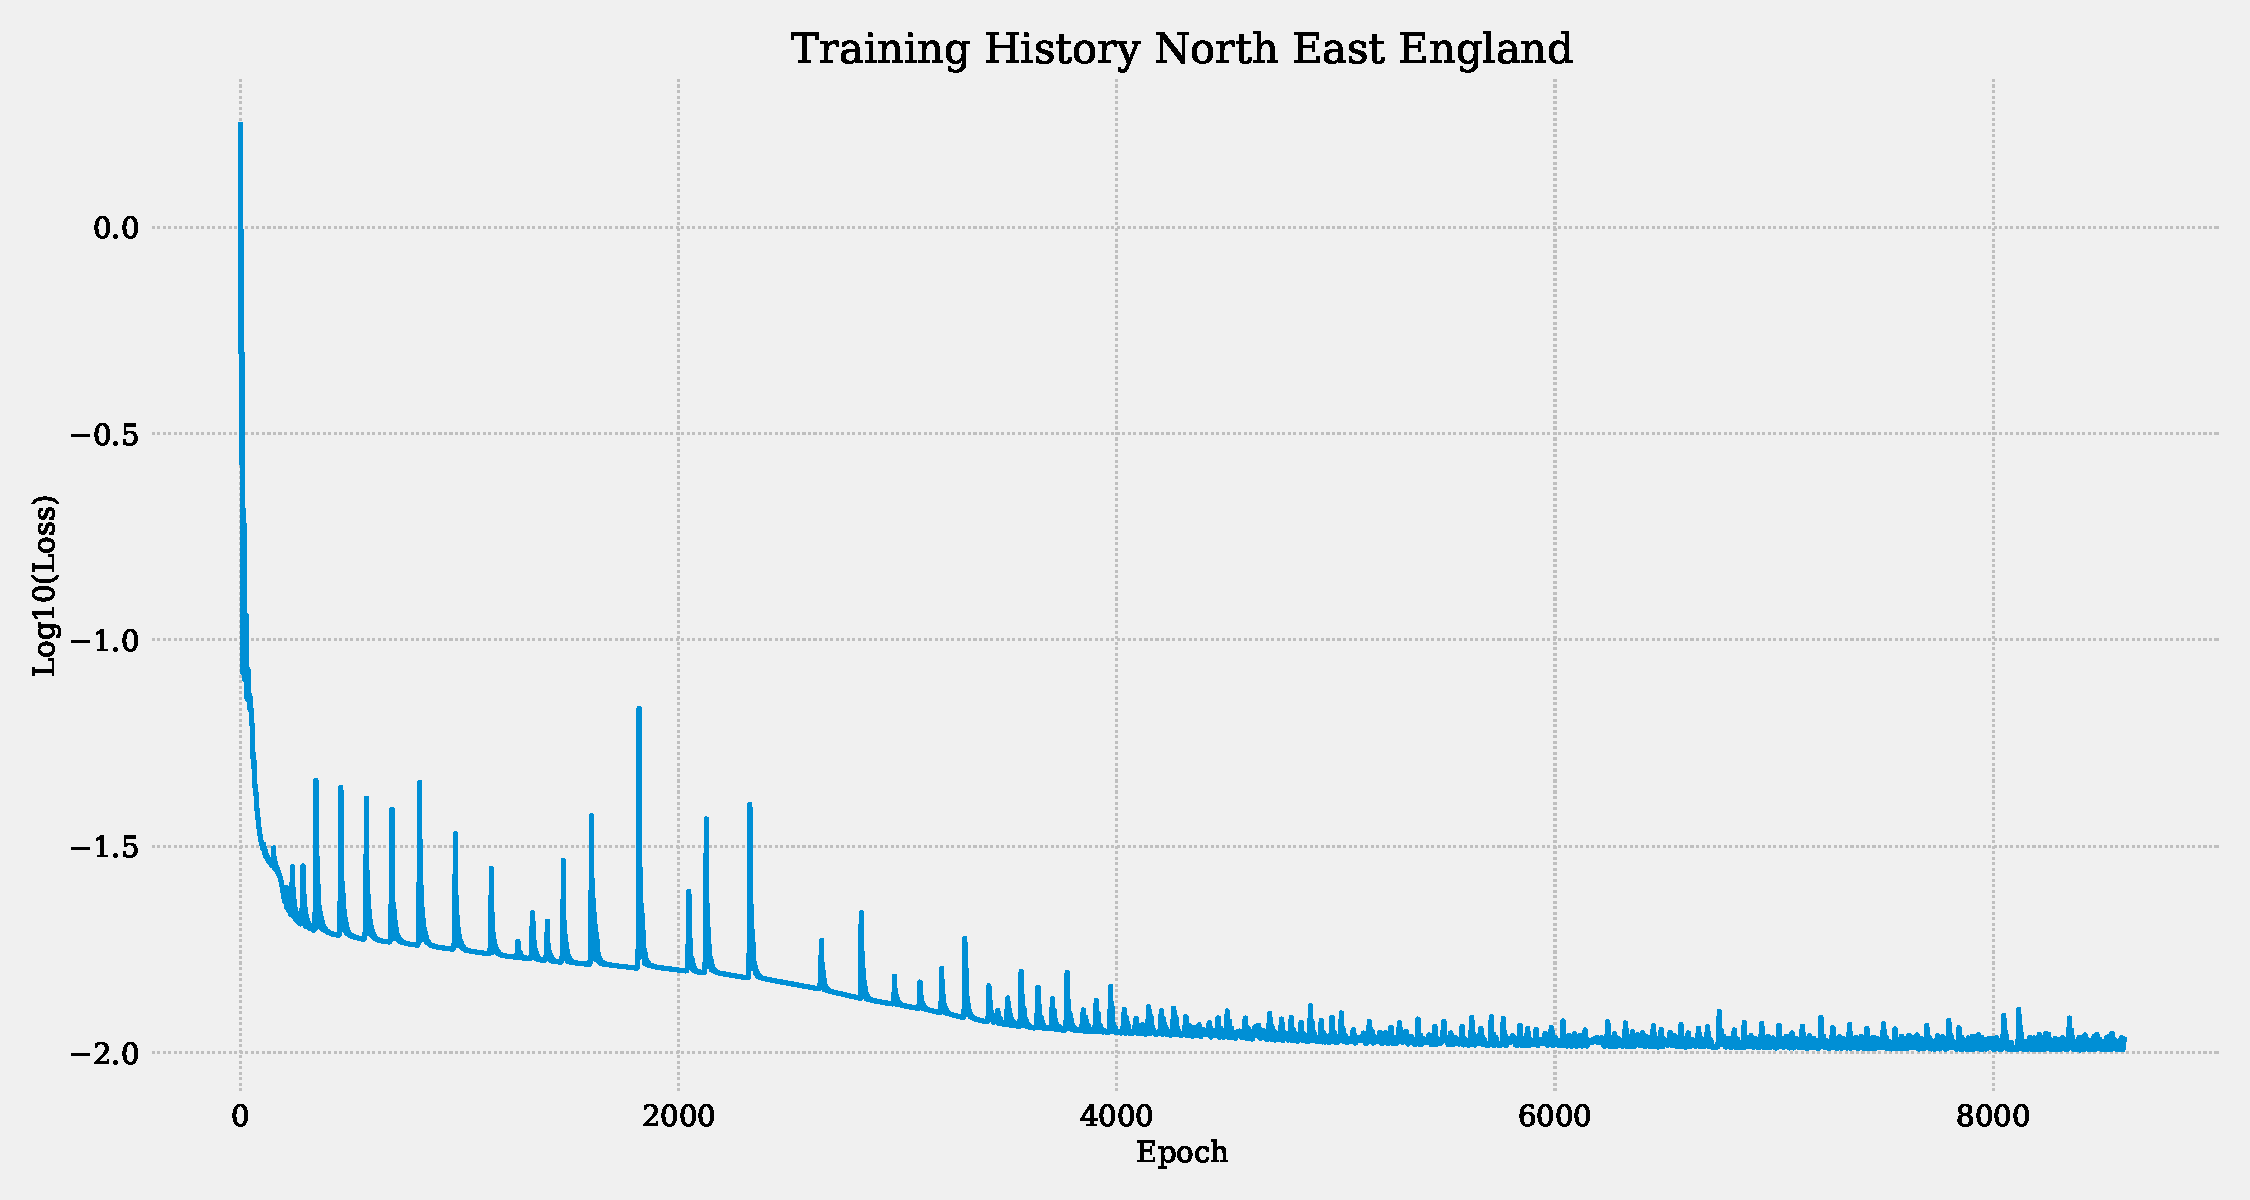
\includegraphics[width=\textwidth]{images/pinn/Training_History_North East England.pdf}
        \caption{Training history of the PINN model}
        \label{fig:Training_History_North East England}
    \end{subfigure}
    \caption{Physics-Informed Neural Network (PINN) model predictions and training history for the North East England region, showcasing the dynamics of susceptible, infectious, and recovered populations alongside model training progression.}
    \label{fig:PINN_North East England_Comprehensive}
\end{figure*}

\begin{figure}
    \centering
    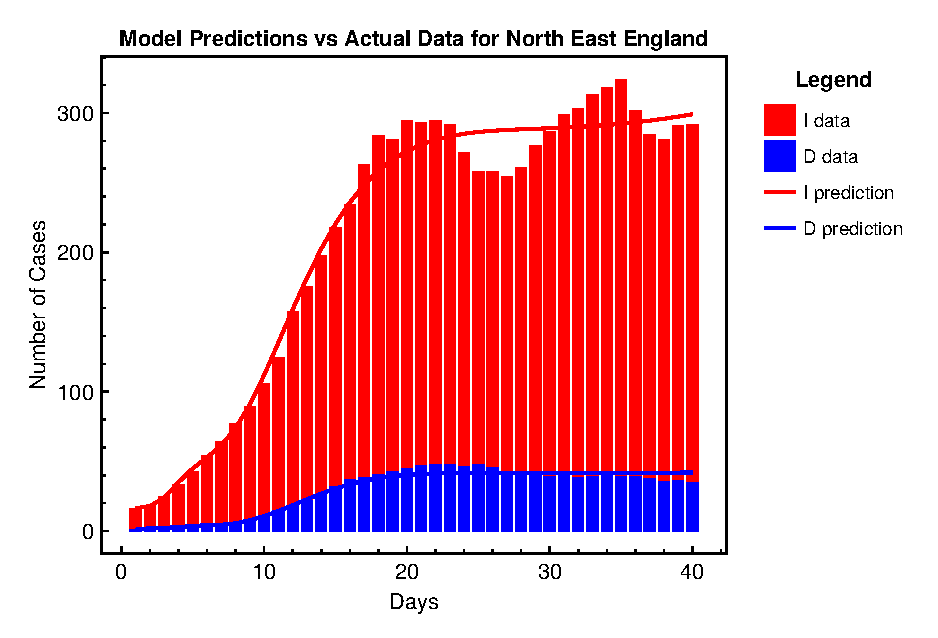
\includegraphics[width=0.8\textwidth]{images/ude/North East England_infected_death_data.pdf}
    \caption{Predicted number of infected and deceased individuals}
    \label{fig:ude_North East England}
\end{figure}


\begin{figure*}
    \centering
    \begin{subfigure}[t]{0.45\textwidth}
        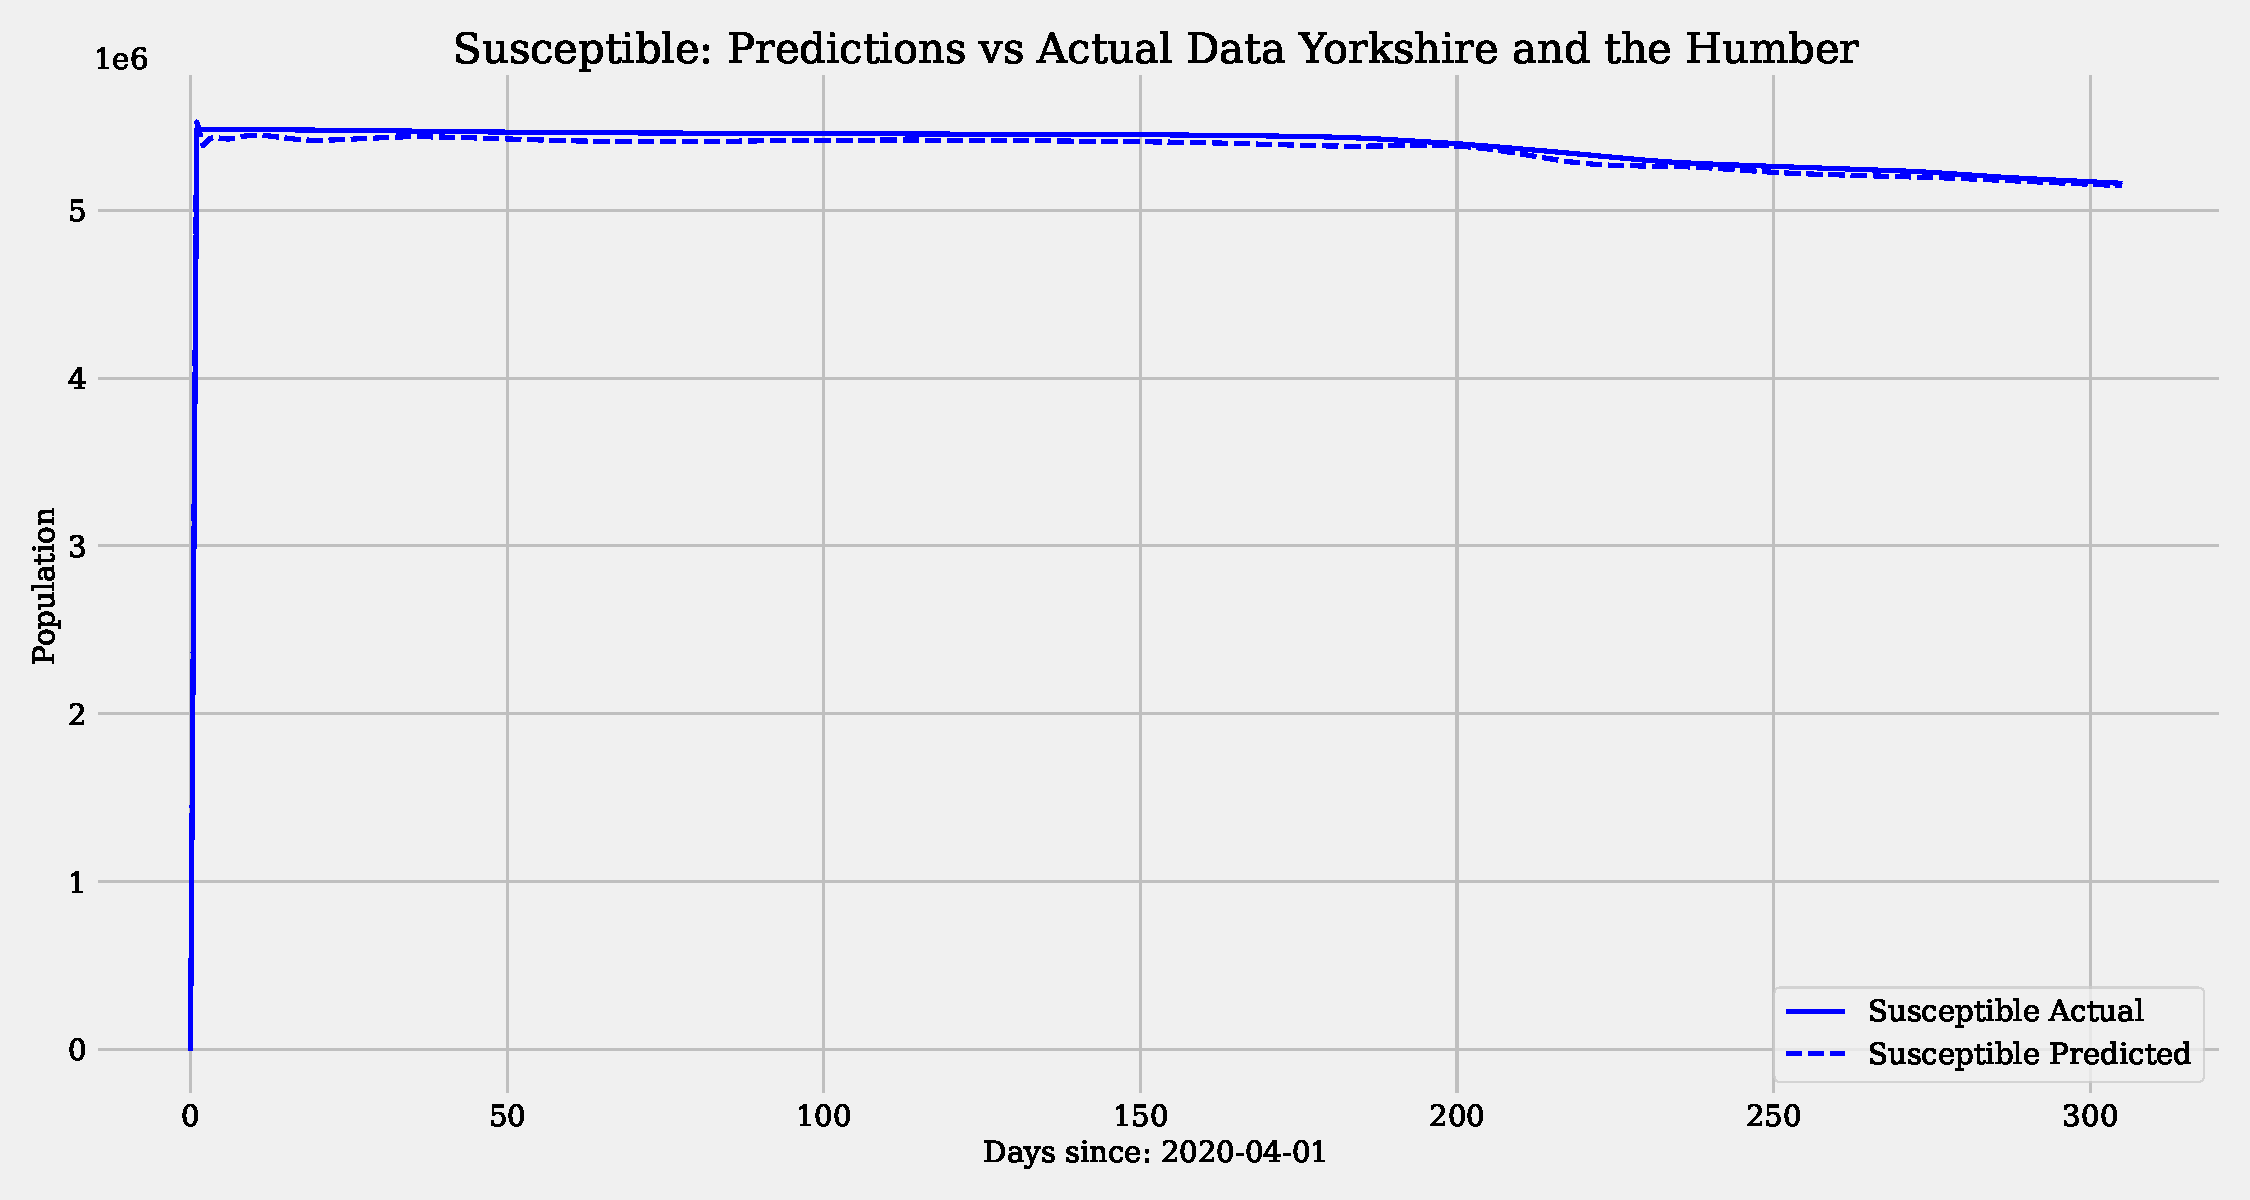
\includegraphics[width=\textwidth]{images/pinn/S_predictions_Yorkshire and the Humber.pdf}
        \caption{Predicted number of susceptible individuals}
        \label{fig:S_predictions_Yorkshire and the Humber}
    \end{subfigure}
    \hfill % Ensures that the figures are spaced out evenly
    \begin{subfigure}[t]{0.45\textwidth}
        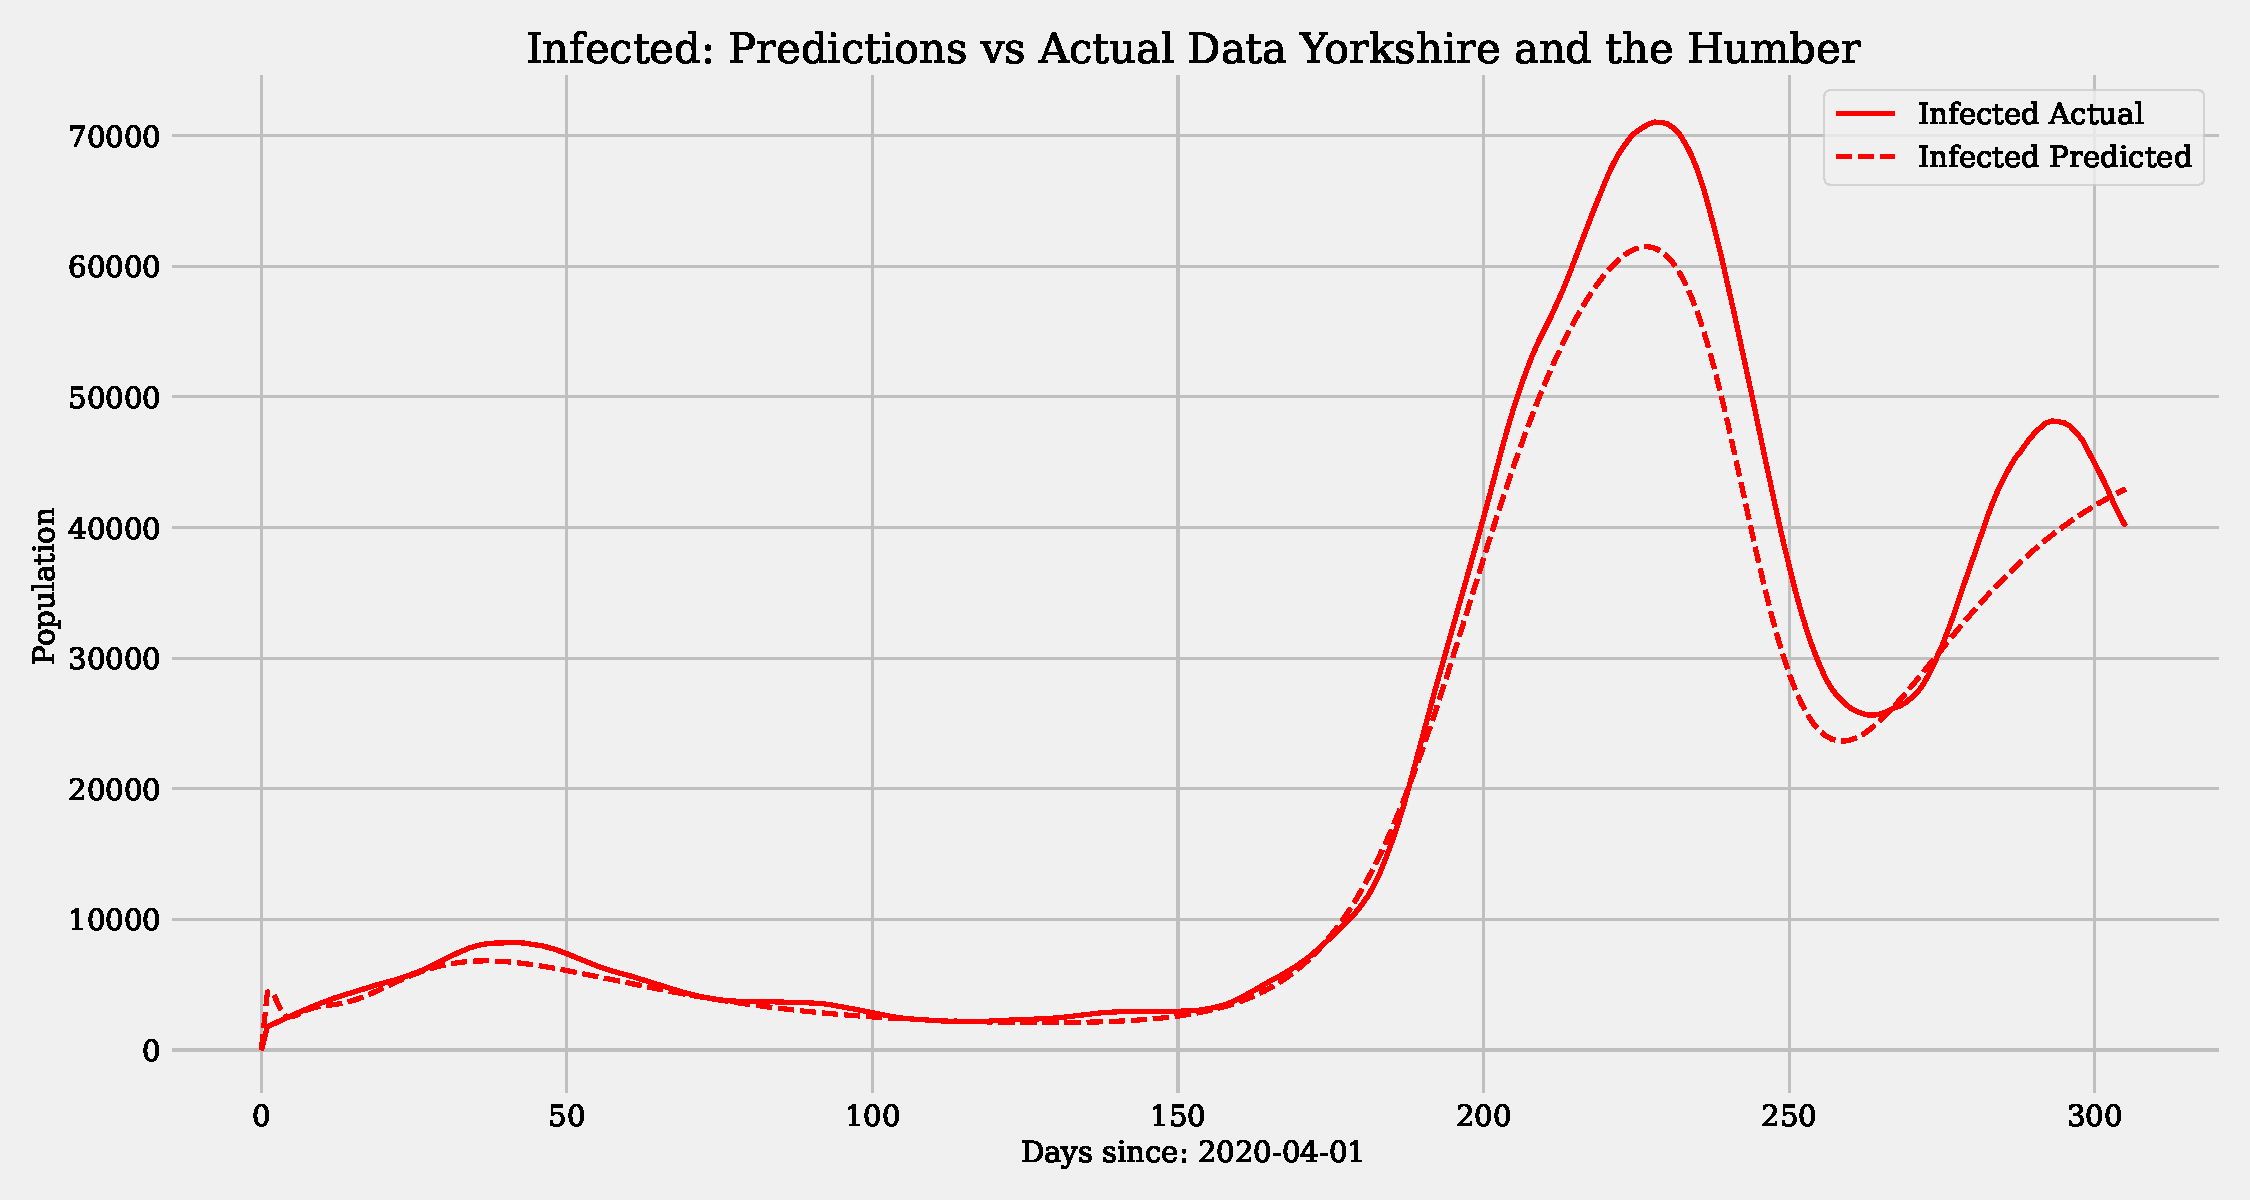
\includegraphics[width=\textwidth]{images/pinn/I_predictions_Yorkshire and the Humber.pdf}
        \caption{Predicted number of infectious individuals}
        \label{fig:I_predictions_Yorkshire and the Humber}
    \end{subfigure}

    % Adds a bit of vertical space between the rows of figures
    \vspace{0.5cm}

    \begin{subfigure}[t]{0.45\textwidth}
        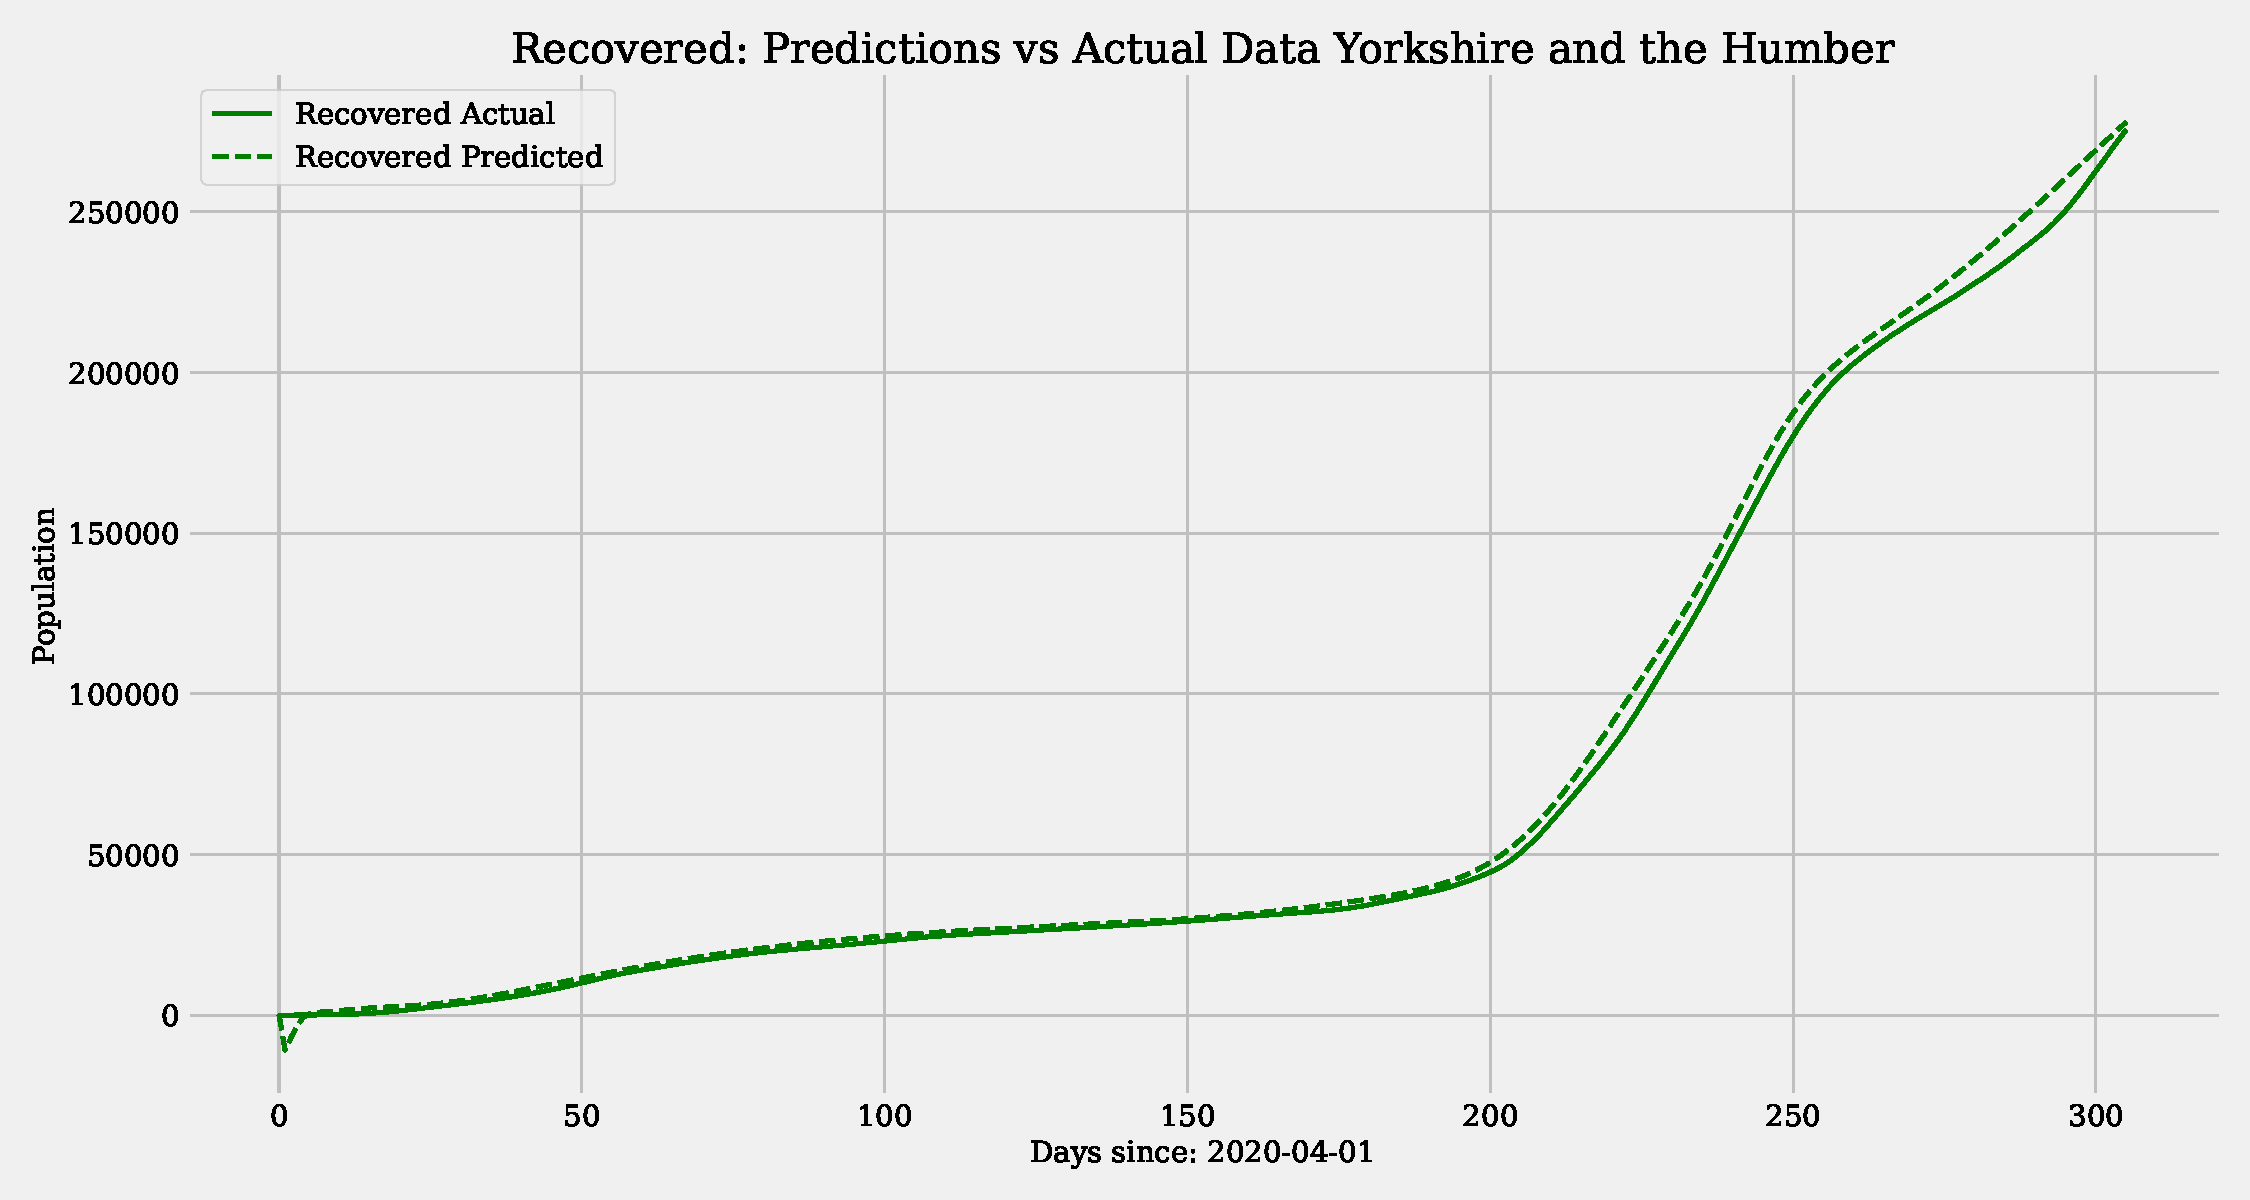
\includegraphics[width=\textwidth]{images/pinn/R_predictions_Yorkshire and the Humber.pdf}
        \caption{Predicted number of recovered individuals}
        \label{fig:R_predictions_Yorkshire and the Humber}
    \end{subfigure}
    \hfill % Ensures that the figures are spaced out evenly
    \begin{subfigure}[t]{0.45\textwidth}
        \centering
        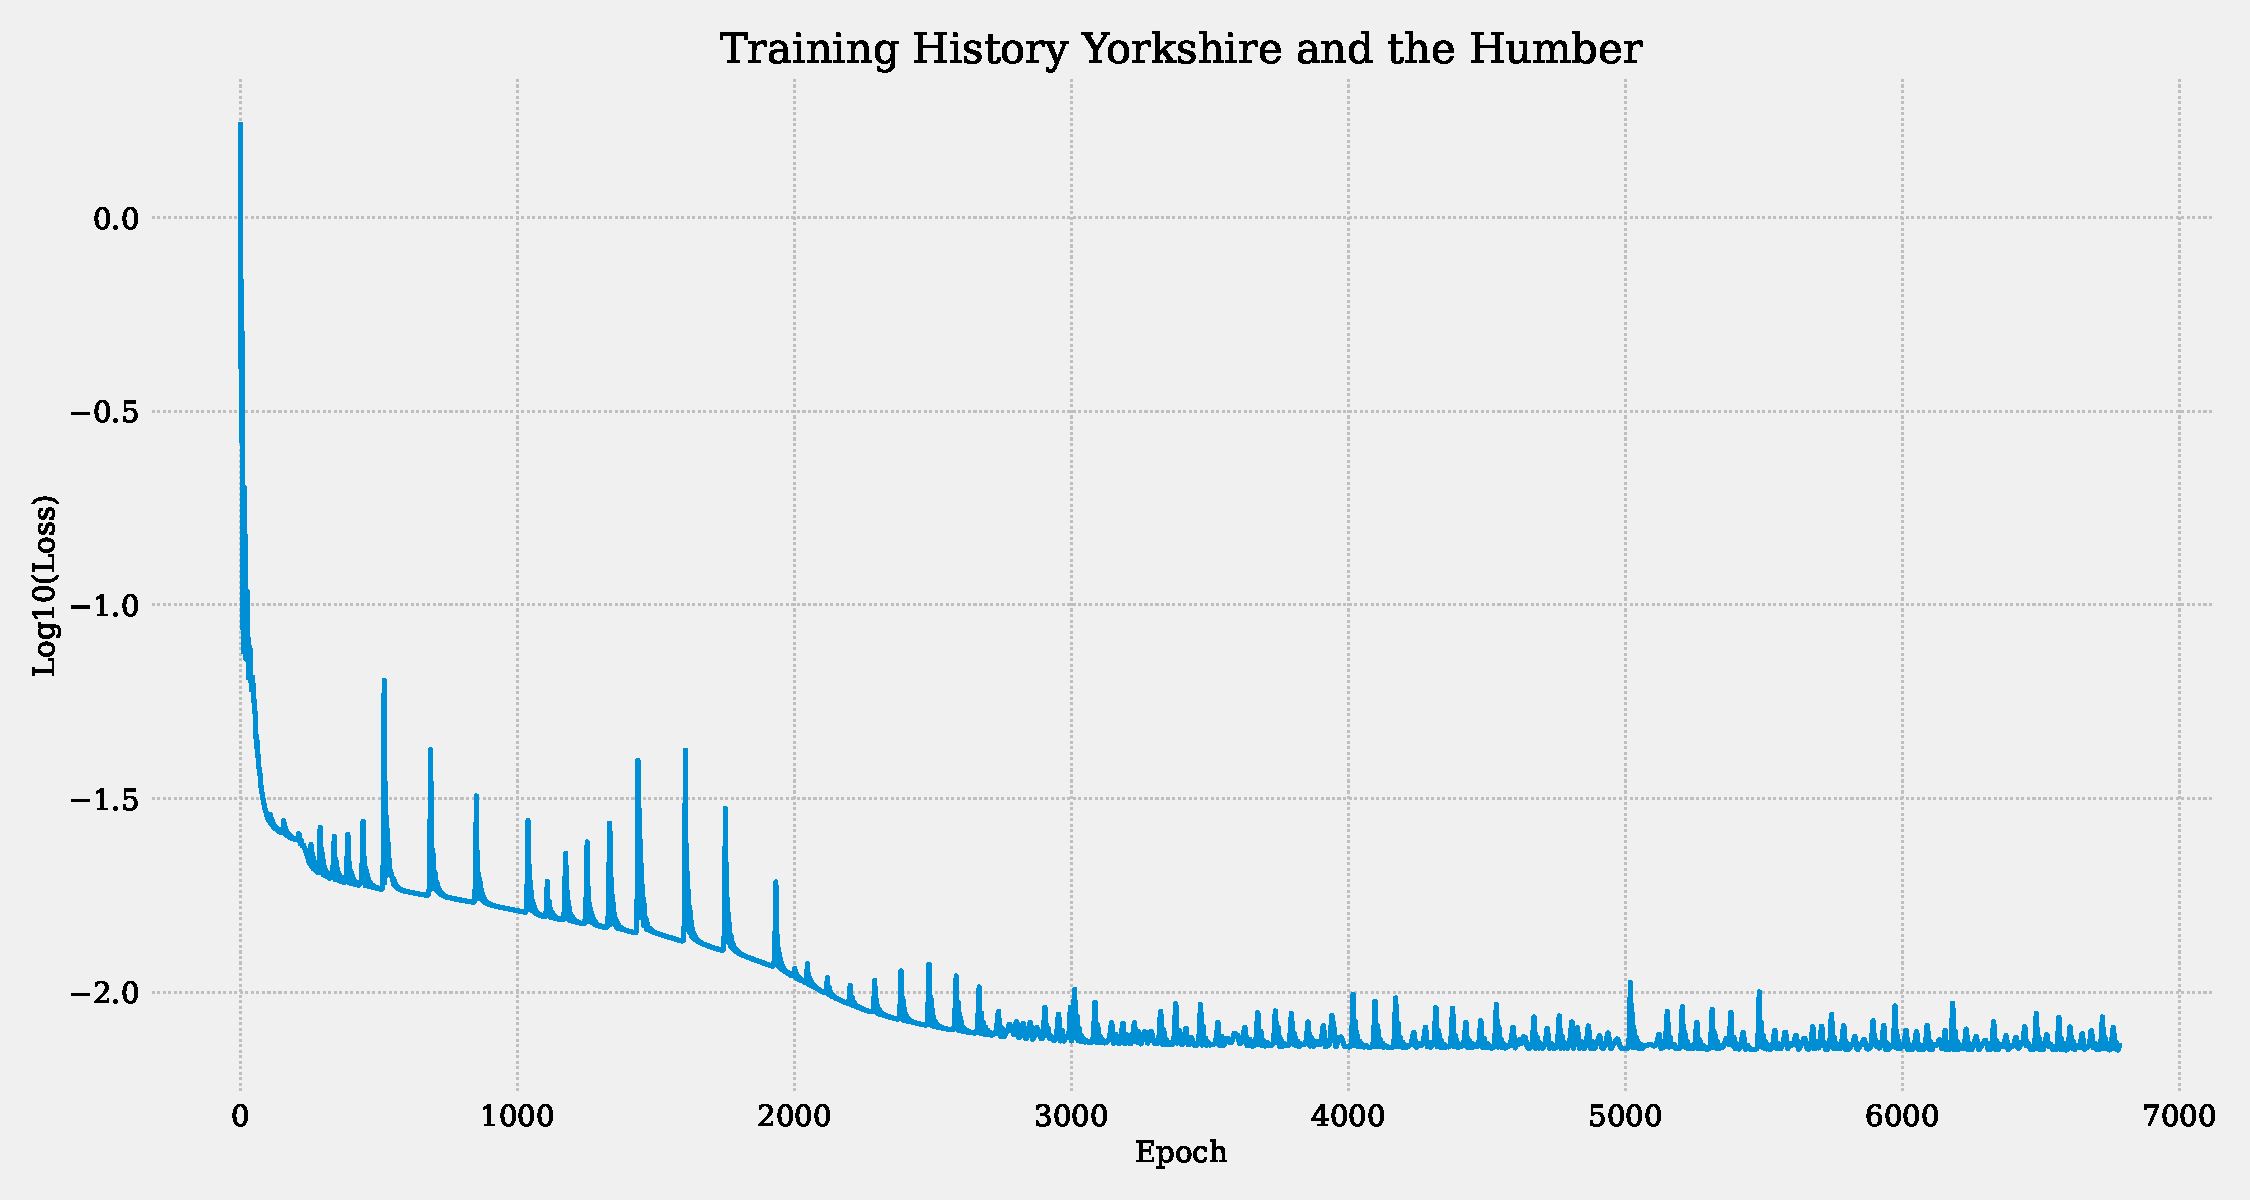
\includegraphics[width=\textwidth]{images/pinn/Training_History_Yorkshire and the Humber.pdf}
        \caption{Training history of the PINN model}
        \label{fig:Training_History_Yorkshire and the Humber}
    \end{subfigure}
    \caption{Physics-Informed Neural Network (PINN) model predictions and training history for the Yorkshire and the Humber region, showcasing the dynamics of susceptible, infectious, and recovered populations alongside model training progression.}
    \label{fig:PINN_Yorkshire and the Humber_Comprehensive}
\end{figure*}


\bibliographystyle{alphaurl}
\bibliography{refs}
\end{document}